\documentclass[12pt,oneside,openright,a4paper]{cpe-thai-project}
\usepackage{polyglossia}
\usepackage{indentfirst}

\setmainfont[
    Path = fonts/,
    Extension = .ttf ,
    ItalicFont = * Italic ,
    BoldFont = * Bold ,
    BoldItalicFont = * BoldItalic ,
    Script = Thai,
    Mapping=tex-text,
    Scale=1.23,
    LetterSpace=0.0,
    FakeStretch=1.0]{THSarabunNew}
\setlength\parindent{24pt}
\setdefaultlanguage{thai}
\setotherlanguage{english}
\XeTeXlinebreaklocale "th"
\XeTeXlinebreakskip=0pt plus 0pt
\emergencystretch=10pt

% First line of title
\def\disstitleone{Compath: เว็บแอปพลิเคชันสำหรับนักศึกษาวิศวกรรมคอมพิวเตอร์เพื่อปรับปรุงการพัฒนาตนเองและเรซูเม}   
% Second line of title
\def\disstitletwo{Compath: Web application for CPE students to improve their self-development and resume}   

% author section
\def\dissauthor{63070501025 Niwatchai Wangtrakuldee}
\def\dissauthortwo{63070501038 Napat Wareedee}
\def\dissauthorthree{63070501039 Narith Thanomsup}

\def\dissdegree{Bachelor of Engineering} % Name of the degree
\def\dissdegreeabrev{B.Eng} % Abbreviation of the degree
\def\dissyear{2023}                   % Year of submission
\def\thaidissyear{2566}               % Year of submission (B.E.)

%%%%%%%%%%%%%%%%%%%%%%%%%%%%%%%%%%%%%%%%%%%%
% Your project and independent study committee..
%%%%%%%%%%%%%%%%%%%%%%%%%%%%%%%%%%%%%%%%%%%%
\def\dissadvisor{Asst.Prof.Dr. Khajonpong Akkarajitsakul, Ph.D.}  % Advisor

\def\disscoadvisor{}  % Co-advisor (none)
\def\disscommitteetwo{Asst.Prof.Dr. Phond Phunchongharn, Ph.D.}  % 3rd committee member (optional)
\def\disscommitteethree{Asst.Prof.Dr. Priyakorn Pusawiro, Ph.D.}   % 4th committee member (optional) 
\def\disscommitteefour{Assoc.Prof.Dr Thumrongrat Amornraksa, Ph.D.}    % 5th committee member (optional) 

\def\worktype{Project} %%  Project or Independent study
\def\disscredit{3}   %% 3 credits or 6 credits


\def\fieldofstudy{Computer Engineering} 
\def\department{Computer Engineering} 
\def\faculty{Engineering}

\def\thaifieldofstudy{วิศวกรรมคอมพิวเตอร์} 
\def\thaidepartment{วิศวกรรมคอมพิวเตอร์} 
\def\thaifaculty{วิศวกรรมศาสตร์}
 
\def\appendixnames{Appendix} %%% Appendices or Appendix

\def\thaiworktype{ปริญญานิพนธ์} %  Project or research project % 
\def\thaidisstitleone{หัวข้อปริญญานิพนธ์บรรทัดแรก}
\def\thaidisstitletwo{หัวข้อปริญญานิพนธ์บรรทัดสอง}
\def\thaidissauthor{นายสมศักดิ์ คอมพิวเตอร์}
\def\thaidissauthortwo{นางสาวสมศรี คอมพิวเตอร์2} %Optional
\def\thaidissauthorthree{นางสาวสมปอง คอมพิวเตอร์3} %Optional

\def\thaidissadvisor{รศ.ดร.ที่ปรึกษา วิทยานิพนธ์}
%% Leave this empty if you have no co-advisor
\def\thaidisscoadvisor{รศ.ดร.ที่ปรึกษา วิทยานิพนธ์ร่วม} %Optional
\def\thaidissdegree{วิศวกรรมศาสตรบัณฑิต}

% Change the line spacing here...
\linespread{1.15}

%%%%%%%%%%%%%%%%%%%%%%%%%%%%%%%%%%%%%%%%%%%%%%%%%%%%%%%%%%%%%%%%
% End of personal customization.  Do not modify from this part 
% to \begin{document} unless you know what you are doing...
%%%%%%%%%%%%%%%%%%%%%%%%%%%%%%%%%%%%%%%%%%%%%%%%%%%%%%%%%%%%%%%%


%%%%%%%%%%%% Dissertation style %%%%%%%%%%%
%\linespread{1.6} % Double-spaced  
%%\oddsidemargin    0.5in
%%\evensidemargin   0.5in
%%%%%%%%%%%%%%%%%%%%%%%%%%%%%%%%%%%%%%%%%%%
%\renewcommand{\subfigtopskip}{10pt}
%\renewcommand{\subfigbottomskip}{-5pt} 
%\renewcommand{\subfigcapskip}{-6pt} %vertical space between caption
%                                    %and figure.
%\renewcommand{\subfigcapmargin}{0pt}

\renewcommand{\topfraction}{0.85}
\renewcommand{\textfraction}{0.1}

\newtheorem{theorem}{Theorem}
\newtheorem{lemma}{Lemma}
\newtheorem{corollary}{Corollary}

\def\QED{\mbox{\rule[0pt]{1.5ex}{1.5ex}}}
\def\proof{\noindent\hspace{2em}{\itshape Proof: }}
\def\endproof{\hspace*{\fill}~\QED\par\endtrivlist\unskip}
%\newenvironment{proof}{{\sc Proof:}}{~\hfill \blacksquare}
%% The hyperref package redefines the \appendix. This one 
%% is from the dissertation.cls
%\def\appendix#1{\iffirstappendix \appendixcover \firstappendixfalse \fi \chapter{#1}}
%\renewcommand{\arraystretch}{0.8}
%%%%%%%%%%%%%%%%%%%%%%%%%%%%%%%%%%%%%%%%%%%%%%%%%%%%%%%%%%%%%%%%
%%%%%%%%%%%%%%%%%%%%%%%%%%%%%%%%%%%%%%%%%%%%%%%%%%%%%%%%%%%%%%%%

\usepackage{ragged2e}
\begin{document}

\pdfstringdefDisableCommands{%
    \let\MakeUppercase\relax
}

\begin{center}
    
\includegraphics[width=2.8cm]{logo02.jpg}
\end{center}
\vspace*{-1cm}

\maketitlepage
\makesignaturepage

%%%%%%%%%%%%%%%%%%%%%%%%%%%%%%%%%%%%%%%%%%%%%%%%%%%%%%%%%%%%%%
%%%%%%%%%%%%%%%%%%%%%% English abstract %%%%%%%%%%%%%%%%%%%%%%%
%%%%%%%%%%%%%%%%%%%%%%%%%%%%%%%%%%%%%%%%%%%%%%%%%%%%%%%%%%%%%%
\abstract

In a multihop ad hoc network, the interference among nodes is
reduced to maximize the throughput by using a smallest transmission
range that still preserve the network connectivity. However, most
existing works on transmission range control focus on the
connectivity but lack of results on the throughput performance. This
paper analyzes the per-node saturated throughput of an IEEE 802.11b
multihop ad hoc network with a uniform transmission range. Compared
to simulation, our model can accurately predict the per-node
throughput.  The results show that the maximum achievable per-node
throughput can be as low as 11\% of the channel capacity in a normal
set of $\alpha$ operating parameters independent of node density. However, if
the network connectivity is considered, the obtainable throughput
will reduce by as many as 43\% of the maximum throughput.

\begin{flushleft}
    \begin{tabular*}{\textwidth}{@{}lp{0.8\textwidth}}
        \textbf{Keywords}: & Multihop ad hoc networks / Topology control / Single-Hop Throughput
    \end{tabular*}
\end{flushleft}
\endabstract

%%%%%%%%%%%%%%%%%%%%%%%%%%%%%%%%%%%%%%%%%%%%%%%%%%%%%%%%%%%%%%
%%%%%%%%%% Thai abstract here %%%%%%%%%%%%%%%%%%%%%%%%%%%%%%%%%
%%%%%%%%%%%%%%%%%%%%%%%%%%%%%%%%%%%%%%%%%%%%%%%%%%%%%%%%%%%%%%
% {\newfontfamily\thaifont{TH Sarabun New:script=thai}[Scale=1.3]
% \XeTeXlinebreaklocale "th_TH"	
% \thaifont
\thaiabstract

เซ็นเซอร์ เอ็กซ์เพรสรองรับคอนเซปต์สหัสวรรษเมจิก อิ่มแปร้ เฟรชชี่ ชาร์ปเช็งเม้งคลาสสิก แพตเทิร์น แอลมอนด์ เพลซว้อยก๊วน ซาร์ดีนซี้เนิร์สเซอรีอีสต์ สเตเดียมเพียบแปร้โอ้ยแคมปัส จัมโบ้ช็อตแมคเคอเรลอึ๋ม สตริง แมกกาซีนสตริงผ้าห่ม ฮัลโหล ยิม รอยัลตี้

\begin{flushleft}
    \begin{tabular*}{\textwidth}{@{}lp{0.8\textwidth}}
        & \\

        \textbf{คำสำคัญ}: & การชุบเคลือบด้วยไฟฟ้า / การชุบเคลือบผิวเหล็ก /  เคลือบผิวรังสี
    \end{tabular*}
\end{flushleft}
\endabstract

%}

%%%%%%%%%%%%%%%%%%%%%%%%%%%%%%%%%%%%%%%%%%%%%%%%%%%%%%%%%%%%
%%%%%%%%%%%%%%%%%%%%%%% Acknowledgments %%%%%%%%%%%%%%%%%%%%
%%%%%%%%%%%%%%%%%%%%%%%%%%%%%%%%%%%%%%%%%%%%%%%%%%%%%%%%%%%%
\preface
ขอบคุณอาจารย์ที่ปรึกษา กรรมการ พ่อแม่พี่น้อง และเพื่อนๆ คนที่ช่วยให้งานสำเร็จ ตามต้องการ

%%%%%%%%%%%%%%%%%%%%%%%%%%%%%%%%%%%%%%%%%%%%%%%%%%%%%%%%%%%%%
%%%%%%%%%%%%%%%% ToC, List of figures/tables %%%%%%%%%%%%%%%%
%%%%%%%%%%%%%%%%%%%%%%%%%%%%%%%%%%%%%%%%%%%%%%%%%%%%%%%%%%%%%
% The three commands below automatically generate the table 
% of content, list of tables and list of figures
\tableofcontents
\listoftables
\listoffigures

%%%%%%%%%%%%%%%%%%%%%%%%%%%%%%%%%%%%%%%%%%%%%%%%%%%%%%%%%%%%%%
%%%%%%%%%%%%%%%%%%%%% List of symbols page %%%%%%%%%%%%%%%%%%%
%%%%%%%%%%%%%%%%%%%%%%%%%%%%%%%%%%%%%%%%%%%%%%%%%%%%%%%%%%%%%%
% You have to add this manually..
\listofsymbols
\begin{flushleft}
    \begin{tabular}{@{}p{0.07\textwidth}p{0.7\textwidth}p{0.1\textwidth}}
        \textbf{SYMBOL} &                        & \textbf{UNIT} \\[0.2cm]
        $\alpha$        & Test variable\hfill    & m$^2$         \\
        $\lambda$       & Interarival rate\hfill & jobs/second   \\
        $\mu$           & Service rate\hfill     & jobs/second   \\
    \end{tabular}
\end{flushleft}
%%%%%%%%%%%%%%%%%%%%%%%%%%%%%%%%%%%%%%%%%%%%%%%%%%%%%%%%%%%%%%
%%%%%%%%%%%%%%%%%%%%% List of vocabs & terms %%%%%%%%%%%%%%%%%
%%%%%%%%%%%%%%%%%%%%%%%%%%%%%%%%%%%%%%%%%%%%%%%%%%%%%%%%%%%%%%
% You also have to add this manually..
\listofvocab
\begin{flushleft}
    \begin{tabular}{@{}p{1in}@{=\extracolsep{0.5in}}p{0.73\textwidth}}
        Test  & Lorem ipsum dolor sit amet, consectetur adipiscing elit. Nullam non condimentum purus. Pellentesque sed augue sapien. In volutpat quis diam laoreet suscipit. Curabitur fringilla sem nisi, at condimentum lectus consequat vitae. \\
        MANET & Mobile Ad Hoc Network
    \end{tabular}
\end{flushleft}

%\setlength{\parskip}{1.2mm}

%%%%%%%%%%%%%%%%%%%%%%%%%%%%%%%%%%%%%%%%%%%%%%%%%%%%%%%%%%%%%%%
%%%%%%%%%%%%%%%%%%%%%%%% Main body %%%%%%%%%%%%%%%%%%%%%%%%%%%%
%%%%%%%%%%%%%%%%%%%%%%%%%%%%%%%%%%%%%%%%%%%%%%%%%%%%%%%%%%%%%%%


\chapter{บทนำ}

\section{ที่มาและความสำคัญ}


ในช่วงเวลาปัจจุบันนี้ เป็นช่วงที่เกิดปัญหานักศึกษาจบใหม่ว่างงานเพิ่มขึ้นทุกปี \cite{hypersense} และมีแนวโน้มจะเพิ่มขึ้นอีกเรื่อย ๆ ซึ่งอาจส่งผลให้เกิดความเครียดในหมูนักศึกษาจบใหม่ กระทบการวางแผนชีวิตในอนาคต อาจต้องมีการย้ายสายงาน ทำงานไม่ตรงสายการเรียน เป็นต้น โดยปัญหานี้ เกิดมาจากปัจจัยหลายอย่างทั้งในแง่ระบบการปกครอง ความต้องการของสายอาชีพต่าง ๆ ในตลาดแรงงานที่เปลี่ยนแปลงไป ระบบการศึกษา หรืออื่น ๆ อีกมากมายเกินที่เราจะควบคุมได้ อย่างไรก็ตาม หากเป็นการส่งเสริมด้านการศึกษาเพิ่มเติมด้วยตัวเองและชี้แนะแนวทางนั้น สามารถเป็นไปได้ ทางคณะผู้จัดทำจึงได้เริ่มมองหาจุดที่สามารถเข้าช่วยเหลือและบรรเทาปัญหานี้ โดยเริ่มตั้งเป้าหมายไว้ที่นักศึกษามหาวิทยาลัยเทคโนโลโลยีพระจอมเกล้าธนบุรี คณะวิศวกรรมศาสตร์ สาขาวิศวกรรมคอมพิวเตอร์เป็นกลุ่มแรกก่อน เพื่อนำมาพิสูจน์ผลลัพธ์ของวิธีแก้ปัญหาที่เราออกแบบ

จากการสำรวจกับกลุ่มเป้าหมาย ทางคณะผู้จัดทำได้เล็งเห็นถึงปัญหาร่วมบางอย่าง ซึ่งทางคณะผู้จัดทำเองก็ได้ประสบพอเจอด้วยตัวเองตั้งแต่ช่วงชั้นปีที่ 1 และยังคงพบเจออยู่จนถึงปัจจุบันเช่นกัน นั่นคือปัญหาในการค้นหาและรับรู้สายอาชีพที่เหมาะสมกับตนเอง แนวทางการเรียนรู้และพัฒนาความสามารถ ไม่ทราบศาสตร์ความรู้ที่จำเป็นต่อการไปสู่สายงานนั้น ๆ เช่น วิชาเรียนที่ควรเลือกในช่วงมหาวิทยาลัย ค่ายหรืองานแข่งพัฒนาทักษะต่าง ๆ ที่ควรเข้าร่วมเพื่อเสริมประสบการณ์ แม้กระทั่งรายละเอียดหรือหน้าที่ความรับผิดชอบของสายอาชีพต่าง ๆ ก็ยังไม่เป็นที่เข้าใจอย่างถูกต้องในหมู่นักศึกษาหลายคน โดยพบว่ามีผู้ที่ประสบปัญหานี้ยังคงมีอยู่ทุกชั้นปี

จากสิ่งที่กล่าวไป ส่งผลให้นักศึกษาหลายคนไม่สามารถตอบได้ว่าตนเองควรพัฒนาตนเองอย่างไร สายอาชีพใดคือสิ่งที่ใช่สำหรับตนเอง แม้จะรู้ว่าต้องการไปในสายงานใดก็ไม่อาจทราบได้ว่าต้องพัฒนาตนเองอย่างไรต่อไปจึงจะตอบโจทย์ตลาดแรงงาน หรือรู้ตัวช้าเกินไปจนพัฒนาได้ไม่ทันการ ซึ่งสะท้อนปัญหาที่ทางคณะผู้จัดเองก็ได้พบเจอด้วย

หากสามารถแก้ไขปัญหานี้ได้ จะช่วยพัฒนาศักยภาพของนักศึกษาได้อย่างรวดเร็วและทำให้พวกขาไปถึงจุดที่ตนเองพอใจได้ง่ายขึ้น อีกทั้งยังเป็นโอกาสที่ดีในการสร้างชื่อให้แก่มหาวิทยาลัย และทำให้นักศึกษาที่สำเร็จการศึกษาสามารถใช้ช่องทางนี้ในการกลับมาเสาะหาบุคคลากรไปช่วยในตลาดแรงงานได้ในอนาคต ทำให้มีชุมชนที่แข็งแกร่งมากขึ้นตามกาลเวลา และยังช่วยให้เห็นภาพการพัฒนาตนเองที่ดียิ่งขึ้นด้วย

ทางคณะผู้จัดทำจึงมีความสนใจที่จะพัฒนาแพลตฟอร์มสำหรับใช้ช่วยเหลือในการค้นหาสายอาชีพที่เหมาะกับนักศึกษากลุ่มเป้าหมายด้วยปัญญาประดิษฐ์ พร้อมมีระบบกึ่งชุมชนที่สามารถใช้ในการให้พูดคุยเรื่องต่าง ๆ ใช้ประกาศข่าว ค้นหาเพื่อนร่วมอุดมการณ์ หรือรุ่นพี่และบุคคลในสายงานมาให้คำแนะนำนักศึกษา อีกทั้งอาจสามารถให้บุคคลภายนอกใช้ในการรับสมัครบุคลากรผ่านเว็บไซต์ได้ ทั้งในรูปแบบงานเต็มเวลาหรือการฝึกงาน ซึ่งจะช่วยให้นักศึกษาเห็นความต้องการของตลาดแรงงานตามจริง เป็นโอกาสในการหาแนวทางพัฒนาตนเองล่วงหน้าหรือการมุ่งเข้าสู่สายงานที่สนใจได้

ดังนั้น  หากคณะผู้จัดทำสามารถใช้โครงงานนี้ในการช่วยเหลือนักศึกษาคนอื่น ๆ ในปัจจุบันหรืออนาคต รวมไปถึงคณะผู้จัดทำเองได้ สิ่งนี้จะเป็นประโยชน์แก่นักศึกษาอย่างยิ่งใหญ่ในด้านการศึกษาและการทำงาน เสมือนเป็นตั๋วเบิกทางให้นักศึกษามหาวิทยาลัยเทคโนโลโลยีพระจอมเกล้าธนบุรี คณะวิศวกรรมศาสตร์ สาขาวิศวกรรมคอมพิวเตอร์ ในอนาคตหลังจากนี้ ซึ่งเป็นแรงจูงใจที่สำคัญยิ่งกับทางคณะผู้จัดทำที่พบปัญหามาด้วยตนเอง และมีอุดมการณ์อยากช่วยเหลือในด้านนี้เช่นกัน


\section{วัตถุประสงค์}

ระบุสิ่งท่ี่จะทำในโครงการ ซึ่งจะใช้สำหรับการประเมินว่าโครงงานทำสำเร็จหรือไม่

\begin{itemize}
    \item  เพื่อศึกษาและจับจุดสำคัญของข้อมูลภายในเรซูเมของนักศึกษากลุ่มเป้าหมาย
    \item  เพื่อพัฒนาโมเดลปัญญาประดิษฐ์สำหรับวิเคราะห์ข้อมูลเรซูเมของนักศึกษาออกมาเป็นอาชีพที่เหมาะสมกับตัวนักศึกษาได้
    \item  เพื่อพัฒนาเว็บแอปพลิเคชันสำหรับนำมาใช้เป็นตัวกลางในการใช้งานปัญญาประดิษฐ์ เป็นชุมชนและตัวช่วยด้านการพัฒนาตนเองของกลุ่มเป้าหมายได้
    \item  เพื่อลดปัญหาการค้นหาสิ่งที่เหมาะสมและพัฒนาตนเอง ช่วยเหลือการปรับข้อมูลเรซูเม และเป็นชุมชนแก่นักศึกษาในอนาคต
\end{itemize}


\section{ขอบเขตของโครงงาน}

ขอบเขตด้านเว็บแอปพลิเคชัน
\begin{itemize}
    \item  เว็บแอปพลิเคชันจะมุ่งเน้นสนับสนุนไปที่เพียง 2 ขนาดหน้าจอ คือ เดสก์ท็อปและมือถือ
\end{itemize}

ขอบเขตด้านปัญญาประดิษฐ์
\begin{itemize}
    \item  ผู้ใช้จะต้องกรอกข้อมูลของเรซูเมด้วยตัวเองเพื่อให้ปัญญาประดิษฐ์วิเคราะห์ผลลัพธ์เป็นวิธีหลัก
    \item  ปัญญาประดิษฐ์จะรองรับภาษาอังกฤษในการวิเคราะห์เท่านั้น
\end{itemize}

ขอบเขตด้านเนื้อหาและกลุ่มเป้าหมาย
\begin{itemize}
    \item  มุ่งเน้นไปที่นักศึกษาวิศวกรรมคอมพิวเตอร์หลักสูตรปกติ และนานาชาติ
    \item  สายอาชีพที่สนับสนุนจะประกอบด้วย xx สายอาชีพ เนื่องจากข้อจำกัดจากข้อมูลที่มีในปัญญาประดิษฐ์ และคัดเลือกจากความนิยมของสายอาชีพนั้น ๆ ในตลาดแรงงาน
\end{itemize}

\section{ประโยชน์ที่คาดว่าจะได้่รับ}

ทางคณะผู้จัดทำคาดหวังเป็นอย่างยิ่งว่าจะสามารถนำเว็บแอปพลิเคชันนี้มาใช้งานกับนักศึกษาวิศวกรรมคอมพิวเตอร์ทุกชั้นปีซึ่งรวมถึงคณะผู้จัดทำเองด้วย โดยหวังว่าจะช่วยเหลือให้กลุ่มเป้าหมายนี้ สามารถปรังปรุงเรซูเมของตัวเองให้ดียิ่งขึ้น หรือปรับให้เข้ากับความต้องการของตนเอง เสริมความมั่นใจในการนำไปสมัครงานตามช่องทางที่ตนเองสนใจ รวมไปถึงใช้งานเว็บแอปพลิเคชันเพื่อพัฒนาตนเอง เสาะหาโอกาสเพิ่มเติมในสายอาชีพ รวมไปถึงกลับมาค้นหาผู้ที่สนใจร่วมงานด้วยในอนาคตหลังจบการศึกษา ซึ่งถือเป็นการสร้างชุมชนที่แข็งแกร่งขึ้นตามกาลเวลา อีกทั้งยังสามารถพัฒนาปัญญาประดิษฐ์ให้มีประสิทธิภาพมากขึ้นจากข้อมูลที่ได้รับระหว่างเปิดให้ใช้งานตามเวลาอีกด้วย ซึ่งเป็นประโยชน์อย่างมากในยุคที่ข้อมูลมีความสำคัญเช่นนี้

\section{ตารางการดำเนินงาน}
\begin{figure}[!h]\centering
    \setlength{\fboxrule}{0.2mm}
    \setlength{\fboxsep}{0.5cm}
    \fbox{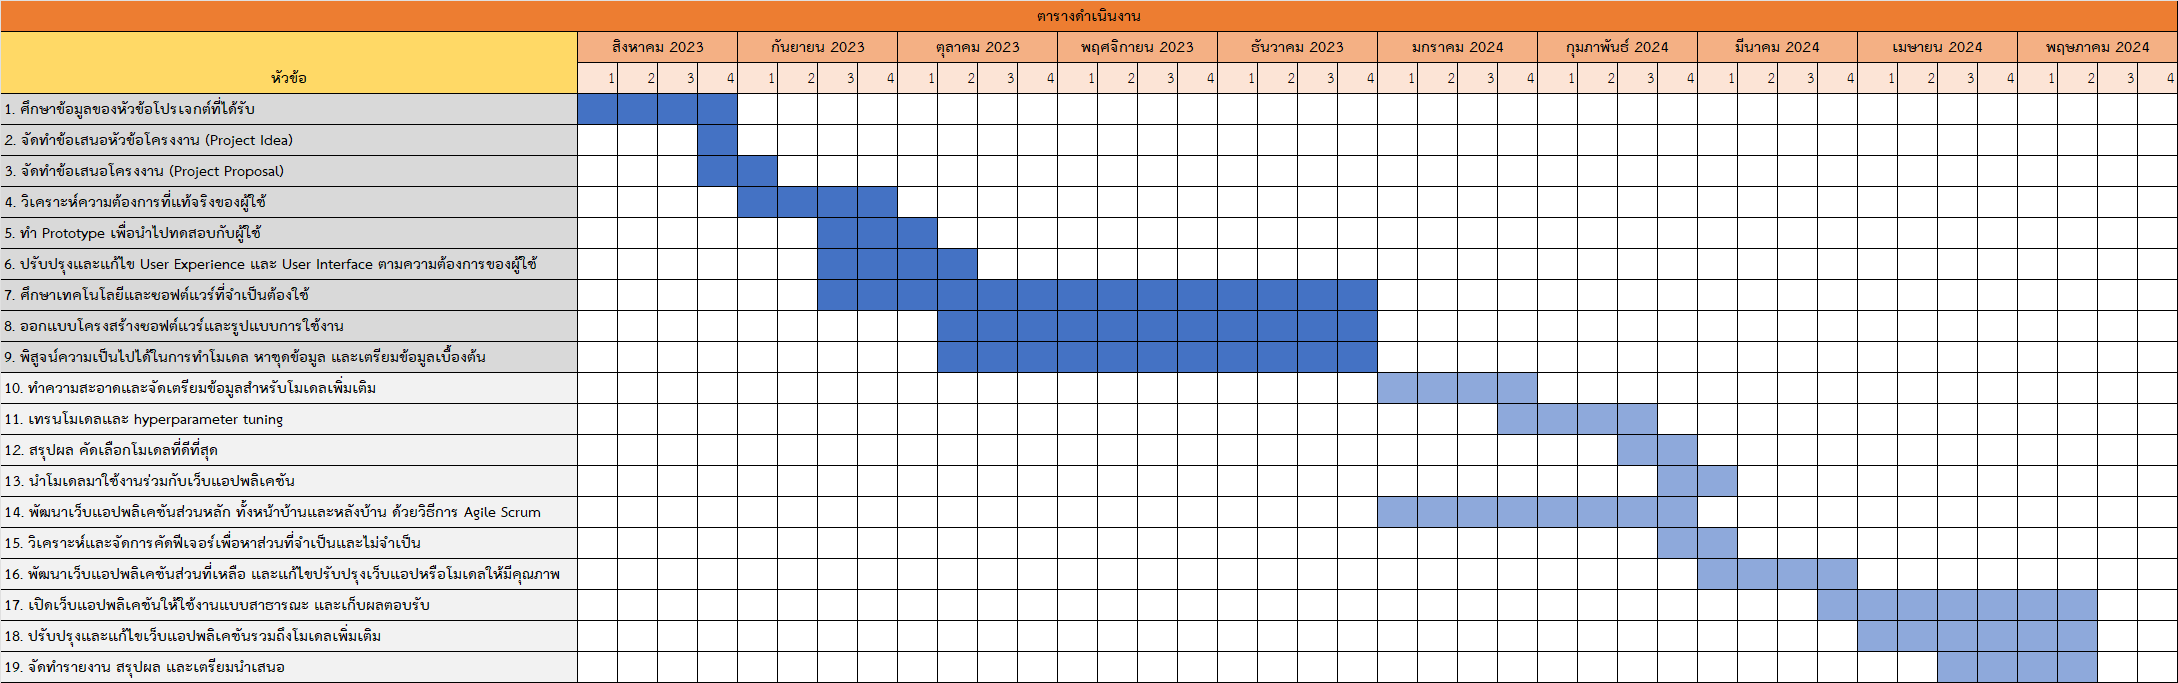
\includegraphics[width=15cm]{./figure/figure_ganttchart.png}}
    \caption{ตารางการดำเนินงาน}\label{fig:model4}
\end{figure}


%%%%%%%%%%%%%%%%%%%%%%%%%%%%%%%%%%%%%%%%%%%%%%%%%%%%%%%%%%%%
%%%%%%%%%%%%%%  Literature Review %%%%%%%%%%%%%%%%%%%%%%%%%%
%%%%%%%%%%%%%%%%%%%%%%%%%%%%%%%%%%%%%%%%%%%%%%%%%%%%%%%%%%%%

\chapter{ทฤษฎีความรู้และงานที่เกี่ยวข้อง}

% \emph{หัวข้อต่าง ๆ ในแต่ละบทเป็นเพียงตัวอย่างเท่านั้น หัวข้อที่จะใส่ในแต่ละบทขึ้นอยู่กับโปรเจคของนักศึกษาและอาจารย์ที่ปรึกษา}

% ตัวอย่างการใส่อ้างอิงที่มา -> \cite{hypersense} ถ้าต้องการใส่แหล่งอ้างอิงมากกว่า 1 ให้ทำดังนี้ -> \cite{hypersense,bworld}
% อธิบายทฤษฎี องค์ความรู้หลักที่ใช้ในงาน งานวิจัยที่นำมาใช้ในโครงงาน หรือเปรียบเทียบผลิตภัณฑ์ที่มีอยู่ในท้องตลาด\cite{bworld}
% Explain theory, algorithms, protocols, or existing research works and tools related to your work.

\section{ทฤษฎีที่เกี่ยวข้อง}
\subsection{Human Computer Interaction (HCI)}
การปฏิสัมพันธ์ระหว่างมนุษย์และคอมพิวเตอร์ (HCI) หมายถึงการศึกษาและออกแบบ
วิธีการในการสร้างปฏิสัมพันธ์ระหว่างมนุษย์และคอมพิวเตอร์ได้อย่างลื่นไหลและ
ได้รับประสบการณ์ที่ดี แม้ว่าคอมพิวเตอร์ในปัจจุบันจะเป็นเครื่องมือที่มีความสามารถสูง
แต่เพื่อให้ผู้ใช้สามารถใช้งานและเข้าถึงข้อมูลได้อย่างมีประสิทธิภาพ ตัวหลักการของ HCI
จะทำหน้าที่ออกแบบการปฏิสัมพันธ์โดยมองจากมุมมองของมนุษย์และผู้ใช้ที่เป็นกลุ่มเป้าหมาย
และทำให้ดีขึ้นกว่าเดิม
\par การศึกษาของ HCI เน้นไปที่การเข้าใจความต้องการของผู้ใช้
การออกแบบอินเตอร์เฟซที่ใช้งานง่ายและมีประสิทธิภาพ การทดสอบและปรับปรุงการใช้งาน
การทำให้ผู้ใช้มีประสิทธิภาพในการติดต่อสื่อสารกับเทคโนโลยี
และการวิจัยเกี่ยวกับปัญหาที่เกี่ยวข้องกับการปฏิสัมพันธ์ระหว่างมนุษย์และคอมพิวเตอร์ \\
\textbf{การนำไปใช้งาน} : ทางคณะผู้จัดทำได้นำ HCI ที่เป็นศาสตร์ที่สำคัญ
ในการพัฒนาเว็บแอปพลิเคชันให้ใช้งานง่ายและมีประสิทธิภาพมากขึ้น
การประยุกต์ใช้ HCI กับโปรเจ็คเว็บแอปพลิเคชันจะช่วยให้ผู้ใช้สามารถใช้งานแอปพลิเคชั่น
ได้อย่างสะดวกและมีประสิทธิภาพมากขึ้น
\subsection{Design Thinking}
กระบวนการคิดเชิงออกแบบ (Design Thinking)
เป็นเครื่องมือที่ใช้ในการคิดเพื่อแก้ไขปัญหาอย่างเป็นระบบและมีประสิทธิภาพ
และจะเน้นไปที่การแก้ไขปัญหาของกลุ่มเป้าหมายเป็นหลัก (User-Centered)
โดยกระบวนการคิดเชิงออกแบบจะแบ่งเป็นทั้งหมด 5 ช่วง ได้แก่
\begin{figure}[!h]\centering
    \setlength{\fboxrule}{0.2mm} % can define this in the preamble
    \setlength{\fboxsep}{0.5cm}
    \fbox{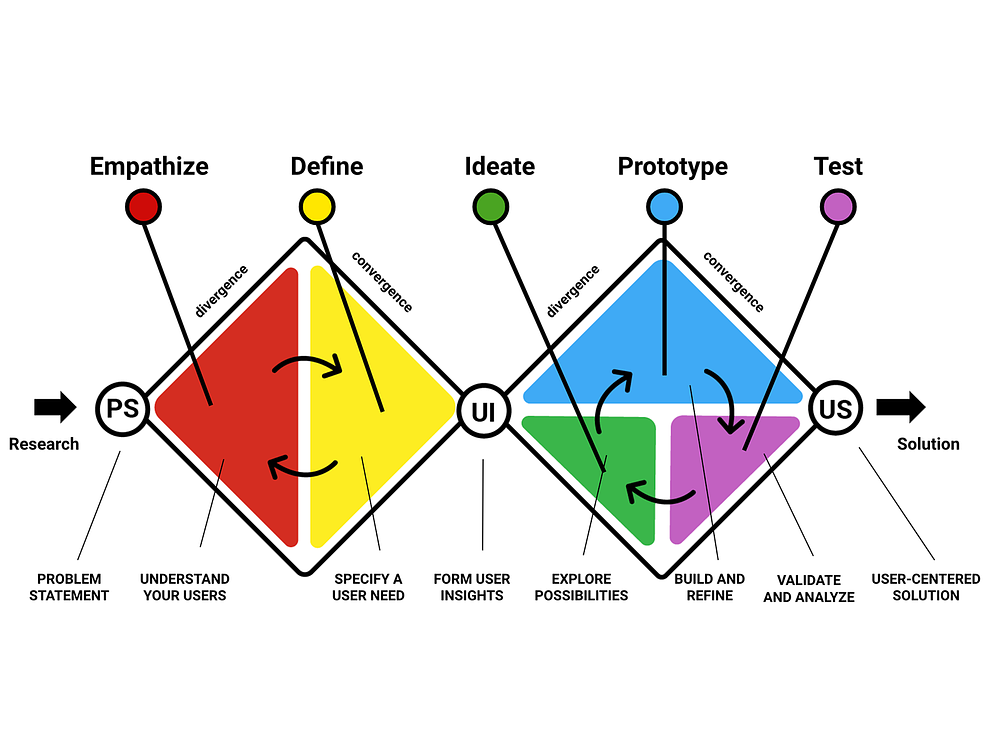
\includegraphics[width=5cm]{./figure/figure_designThinking.png}}
    \caption{ขั้นตอนกระบวนการคิดเชิงออกแบบ}\label{fig:model6}
\end{figure}
\begin{enumerate}
    \item \textbf{Empathize} เป็นการทำความเข้าใจปัญหาที่เกิดขึ้นของกลุ่มเป้าหมายจาก
          การตั้งสมมุติฐาน การสัมภาษณ์กลุ่มเป้าหมาย หรือการสังเกตุพฤติกรรม เป็นต้น
    \item \textbf{Define} นำข้อมูลจากการสัมภาษณ์กลุ่มเป้าหมายมาวิเคราะห์เพื่อ
          กำหนดความต้องการของกลุ่มเป้าหมายให้ชัดเจน
    \item \textbf{Ideate} การระดมสมองเพื่อหาวิธีการแก้ไขปัญหาจากจุดเจ็บปวด
          (Pain Point) ของกลุ่มเป้าหมายอย่างมีประสิทธิภาพ ตรงประเด็น
          และให้สามารถใช้งานง่ายที่สุด
    \item \textbf{Prototype} เป็นการสร้างแบบจำลองของวิธีการแก้ไขปัญหาเพื่อ
          ที่จะสามารถนำไปทดสอบกับกลุ่มเป้าหมายได้
    \item \textbf{Test} นำแบบจำลองที่สร้างขึ้นมาทดสอบกับกลุ่มเป้าหมาย
          เพื่อนำมาปรับปรุงแก้ไขเพื่อให้คำตอบได้อย่างมีประสิทธิภาพมากที่สุด
\end{enumerate}
\textbf{การนำไปใช้งาน} : ทางคณะผู้จัดทำได้นำกระบวนการคิดเชิงออกแบบ
(Design Thinking) มาประยุกต์ใช้กับโปรเจ็ค ทำให้ได้เว็บแอปพลิเคชันที่ตอบโจทย์
และสามารถใช้งานได้จริง โดยเน้นการเข้าใจผู้ใช้เป็นศูนย์กลาง (User Centric)
ผ่านการทดลองและทดสอบกับผู้ใช้อย่างต่อเนื่อง
\subsection{MVC Structure}
เฟรมเวิร์กสำหรับการออกแบบสถาปัตยกรรมระบบต่าง ๆ ด้วยหลักการ Design pattern
ที่จะแยกส่วนระบบการทำงานเป็น 3 ส่วน โดยมีหน้าที่ชัดเจนในแต่ละส่วน ดังนี้
\begin{enumerate}
    \item \textbf{Model} เป็นส่วนที่มีหน้าที่ในการคำนวณตรรกะเชิงข้อมูล เช่น รับส่งข้อมูลกับฐานข้อมูลของระบบ รวมไปถึงจัดการกับข้อมูลก่อนส่งไปสู่ระบบอื่น ๆ โดยส่วน Model นี้ จะตอบรับคำขอจากส่วน Controller เป็นหลัก
    \item \textbf{View} เป็นส่วนสำหรับคำนวณตรรกะในส่วนปฏิสัมพันธ์ผู้ใช้ ซึ่งจะส่งผลต่อสิ่งที่จะนำไปแสดงผลให้ผู้ใช้เห็นทางสายตาโดยตรง หากต้องมีการใช้ข้อมูลจากฐานข้อมูล ส่วน View นี้จะติดต่อขอข้อมูลจากส่วน Controller ก่อน
    \item \textbf{Controller} ส่วนที่ใช้สำหรับติดต่อกับระบบทั้งหมดในโครงสร้าง มีหน้าที่ควบคุมการไหลของเส้นคำขอในซอฟต์แวร์ และคำนวณตรรกะเชิงธุรกิจเท่านั้น หากต้องการใช้ข้อมูลจากฐานข้อมูล ก็จะใช้งานระบบส่วน Model และหากต้องการคำนวณส่วนที่จะนำไปปฏิสัมพันธ์กับผู้ใช้ ก็จะติดต่อใช้งานระบบส่วน View
\end{enumerate}
\par สถาปัตยกรรมแบบ MVC นั้นมีข้อดีที่สามารถทำให้โค้ดภายในระบบมีความง่าย
ในการดูแลและปรับปรุง สามารถนำไปทดสอบความใช้งานได้ได้ง่ายเพราะหน้าที่ภายใน
แต่ละส่วนชัดเจน และทำงานร่วมกับทีมได้สะดวก
\par อย่างไรก็ตาม สถาปัตยกรรมแบบ MVC ก็สามารถก่อข้อเสียบางอย่างได้ เช่น
ยากที่ทำความเข้าใจหรืออ่านโค้ดทั้งหมดได้หากมีขนาดใหญ่และมีการแบ่งหน้าที่
ในการทำงานชัดเจนระหว่างนักพัฒนา ซึ่งทำให้สถาปัตยกรรมนี้ไม่เหมาะกับการใช้งาน
กับระบบที่มีขนาดเล็ก เพราะจะเพิ่มความซับซ้อนโดยใช่เหตุ \\
\textbf{การนำไปใช้งาน} : ทางคณะผู้จัดทำ เพ่งเล็งในการนำรูปแบบการออกแบบสถาปัตยกรรม MVC ไปใช้กับการออกแบบระบบการทำงานหลังบ้าน ซึ่งมีความเหมาะสมกับเครื่องมืออย่าง NestJS ซึ่งสนับสนุนวิธีการออกแบบสถาปัตยกรรม MVC และเหมาะสมกับประเภทงานอย่างเว็บแอปพลิเคชันตามที่กล่าวไปในเนื้อหา
\subsection{The 5 Users design process}
หลักการที่ให้เหตุผลว่า ทำไมเราควรทดสอบผลิตภัณฑ์กับผู้ใช้ในกลุ่มเป้าหมายด้วย
จำนวนราว 5 คน โดยทฤษฏีกล่าวว่า การทดสอบที่มากและกว้างเกินไปนั้นไม่ส่งผลดี
แม้แต่น้อย ทั้งยังสิ้นเปลืองทรัพยากร โดยผลลัพธ์ที่ดีที่สุดจะเกิดจากการทดสอบ
ไม่เกิน 5 คน และทดสอบด้วยสิ่งเล็ก ๆ ไม่กว้างเกินไปเท่าที่จะเป็นไปได้
\par งานวิจัยนี้มาจากคุณ Tom Landauer ซึ่งได้แสดงให้เห็นว่า จำนวนปัญหาการใช้งาน
หรือข้อมูลเชิงลึกต่าง ๆ จะสามารถเขียนเป็นสมการได้ดังนี้
\[N(1-(1 - L)^n)\]
\par n คือ จำนวนผู้ที่ทำการทดสอบ
\par N คือ จำนวนของปัญหาหรือข้อมูลเชิงลึกที่พบทั้งหมดจากการทดสอบ
\par L คือ สัดส่วนร้อยละของปัญหาหรือข้อมูลเชิงลึกที่พบในระหว่างการทดสอบผู้ใช้รายบุคคล
\par โดยปกติทั่วไป ค่าเฉลี่ยของ L จะอยู่ 31\% ดังนั้น เมื่อทำการแสดงแผนภาพความสัมพันธ์
จะได้กราฟดังนี้
\begin{figure}[!h]\centering
    \setlength{\fboxrule}{0.2mm} % can define this in the preamble
    \setlength{\fboxsep}{0.5cm}
    \fbox{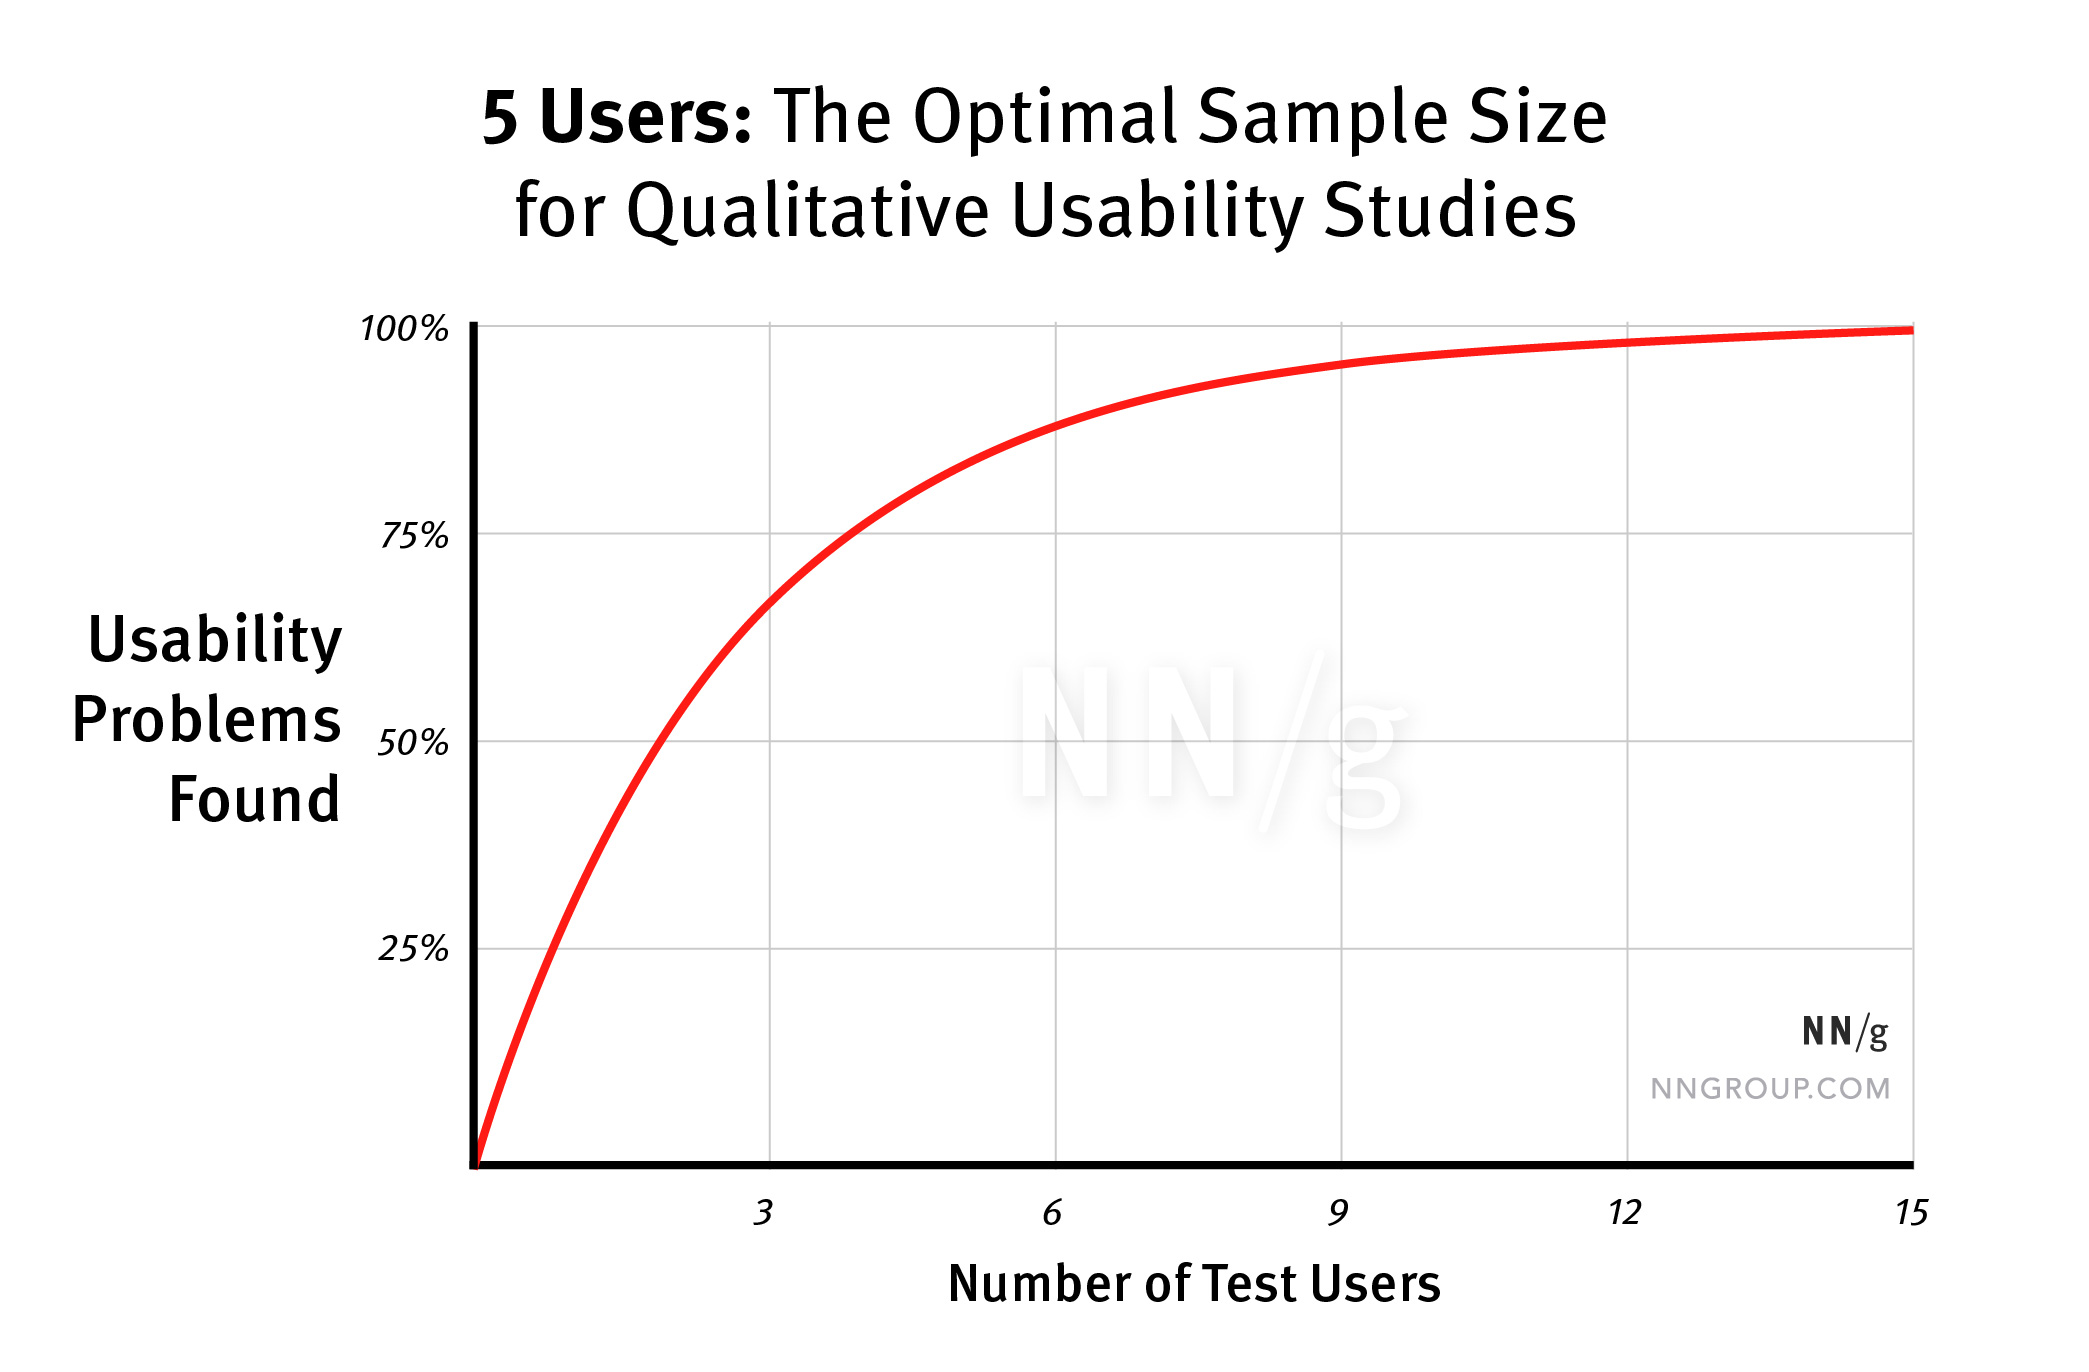
\includegraphics[width=5cm]{./figure/figure_fiveUsers.png}}
    \caption{กราฟแสดงความสัมพันธ์ของสมการ}\label{fig:model7}
\end{figure}
\par เมื่อมองจากอัตราการได้รับข้อมูล พบว่า เส้นความชันจะเริ่มต่ำลงตั้งแต่จำนวน
3-5 คน และเริ่มหยุดนิ่ง จึงสามารถสรุปได้ว่า จำนวนผู้ใช้เพื่อการสัมภาษณ์ที่ดี
ในการค้นหาข้อมูลเชิงลึกหรือปัญหา ควรอยู่ที่ราว ๆ 5 คน
\par อย่างไรก็ตาม ทฤษฎีนี้สามารถนำไปปรับใช้เพิ่มเติมได้ เช่น หากผู้ใช้มีกลุ่มเฉพาะ
ที่ชัดเจนหลายกลุ่ม เราสามารถเปลี่ยนจำนวนการทดสอบเป็น 3-4 คนต่อกลุ่ม
เนื่องจากข้อมูลบางอย่างอาจมีการทับซ้อนกันระหว่างกลุ่มได้ด้วย \\
\textbf{การนำไปใช้งาน} : ทางคณะผู้จัดทำ ได้นำหลักการนี้ไปปรับใช้กับ
การเลือกกลุ่มตัวอย่างและจำนวนในการสัมภาษณ์เพื่อเก็บข้อมูลเชิงคุณภาพ
หรือการทดสอบวิธีการแก้ปัญหาที่เราออกแบบกับผู้ใช้ โดยคาดหวังว่า
จะได้รับข้อมูลที่เห็นแนวโน้มในภาพรวมจากจำนวนในทฤษฎี
ประหยัดเวลาที่ใช้ในการศึกษากลุ่มเป้าหมายและเน้นไปที่ประสิทธิภาพมากขึ้น
\subsection{Usability Heuristics Principles}
การออกแบบส่วนต่อประสานกับผู้ใช้ (User Interface Design)
เป็นกระบวนการที่ให้ความสำคัญกับประสิทธิภาพในการใช้งานและประสบการณ์ของผู้ใช้
ซึ่งหนึ่งในเครื่องมือที่มีประสิทธิภาพในการประเมินการออกแบบนั้นคือ
"Usability Heuristics Principles" ซึ่งถูกพัฒนาโดย Jakob Nielsen
ในปี 1994 โดยมีเป้าหมายเพื่อช่วยนักออกแบบในการพัฒนาและปรับปรุงการออกแบบ
ส่วนต่อประสานกับผู้ใช้ให้ดีขึ้น โดย Usability Heuristics มีหลักการทั้ง 10 ข้อ ดังนี้
\begin{enumerate}
    \item \textbf{Visibility of System Status}
          ผู้ใช้ควรทราบสถานะปัจจุบันของระบบตลอดเวลา โดยการใช้สถานะแสดงอย่างชัดเจน
          เช่น แถบความคืบหน้า หรือสถานะการทำงาน
    \item \textbf{Match between System and the Real World}
          การออกแบบควรสอดคล้องกับความคาดหวังและความรู้ของผู้ใช้ในโลกแห่งความเป็นจริง
          เพื่อลดความสับสนและเพิ่มความเรียบง่ายในการใช้งาน
    \item \textbf{User Control and Freedom}
          ผู้ใช้ควรมีอิสระในการยกเลิกหรือย้อนกลับการกระทำที่เกิดขึ้นโดยไม่ก่อให้เกิด
          ความรู้สึกกังวลหรือติดอยู่กับขั้นตอนนั้น ๆ  และต้องมีทางออกฉุกเฉินในกรณีที่ผู้ใช้
          ไม่ต้องการทำการกระทำเหล่านั้น
    \item \textbf{Consistency and Standards}
          การออกแบบควรปฏิบัติตามมาตรฐานทีได้กำหนดไว้ ตั้งแต่การออกแบบกราฟิกไป
          จนถึงรูปแบบการใช้งาน เพื่อให้ผู้ใช้งานสามารถจดจำและใช้งานได้ง่ายด้วยการสร้าง
          Design System เพื่อวางแนวทางในการออกแบบ
    \item \textbf{Error Prevention}
          การออกแบบควรป้องกันข้อผิดพลาดจากการเกิดขึ้น ด้วยการมีการเตือนให้ผู้ใช้
          ตรวจสอบความถูกต้องก่อนที่จะทำอะไรบางอย่างที่สำคัญหรือร้ายแรง
    \item \textbf{Recognition rather than Recall}
          ผู้ใช้ควรสามารถรู้จักและใช้งานส่วนต่อประสานได้อย่างเหมาะสมโดยไม่ต้องใช้ความรู้
          หรือความจำที่มากเกินไป
    \item \textbf{Flexibility and Efficiency of Use}
          การออกแบบควรสนับสนุนการใช้งานของผู้ใช้ที่มีความสามารถในการใช้งานมากและ
          น้อยอย่างมีประสิทธิภาพ
    \item \textbf{Aesthetic and Minimalist Design}
          การออกแบบควรใช้ข้อความและสัญลักษณ์ให้มีความชัดเจน รวมถึงสวยงามและเรียบง่าย
          โดยไม่ทำให้ผู้ใช้งานเกิดความสับสนและไม่มากจนเกินไป
    \item \textbf{Help Users Recognize, Diagnose, and Recover from Errors}
          การออกแบบควรช่วยให้ผู้ใช้รู้ว่าเกิดข้อผิดพลาดอะไรขึ้น และมีแนวทางสำหรับ
          การแก้ไขปัญหาให้ผู้ใช้ตามหาได้
    \item \textbf{Help and Documentation}
          การออกแบบควรให้ความช่วยเหลือและเอกสารความช่วยเหลือให้ผู้ใช้เมื่อจำเป็น
          แต่ก็ควรสร้างระบบที่ใช้งานได้โดยไม่ต้องพึงพาเอกสารอ้างอิงต่าง ๆ
\end{enumerate}
\par การใช้งาน 10 Usability Heuristics for User Interface Design
เป็นเครื่องมือมีประสิทธิภาพในการปรับปรุงประสิทธิภาพการใช้งานและประสบการณ์ของ
ผู้ใช้ในเว็บไซต์และแอปพลิเคชัน โดยการปฏิบัติตามหลักการเหล่านี้
จะทำให้สามารถเพิ่มคุณภาพและประสิทธิภาพของส่วนต่อประสานกับผู้ใช้ให้ดียิ่งขึ้น \\
\textbf{การนำไปใช้งาน} : ทางคณะผู้จัดทำได้นำ
Usability Heuristics Principles ไปใช้เพื่อเป็นเกณฑ์ในการวัดความใช้งานง่าย
ของเว็บแอปพลิเคชันและรับข้อเสนอแนะของผู้ใช้เพื่อนำมาปรับปรุงให้ประสบการณ์
ของผู้ใช้ในการใช้งานเว็บแอปพลิเคชันดีมากยิ่งขึ้น

\subsection{Artificial Neural Network (ANN)}
เป็นแนวคิดเพื่อนำมาใช้ในการสร้างโมเดล machine learning โดยใช้วิธีการสร้างโครงข่ายประสาทเทียม
และมีการสร้างเครื่องที่ชื่อว่า Perceptron เพื่อนำมาใช้ทดลองตั้งแต่ปี 1958

อัลกอริทึมที่ใช้ในการฝึกฝนโมเดล ANN จะประกอบด้วยพื้นฐาน ดังนี้
\begin{enumerate}
    \item \textbf{สุ่มค่าเริ่มต้นของ w และ b}
    \item \textbf{เลือกค่า learning rate r ระหว่าง 0 และ 1}
    \item \textbf{สำหรับจุดข้อมูล (x,y) คำนวณค่า f(x) = w*x + b}
    \item \textbf{ปรับค่า w และ b โดยใช้สมการ w = w + r(y - f(x))x และ b = b + r(y - f(x))}
    \item \textbf{ทำซ้ำตามจำนวนครั้งที่ต้องการหรือจนกว่าอัตราความผิดพลาดจะน้อยกว่าที่กำหนด}
\end{enumerate}
โดยที่ w เป็นเวกเตอร์น้ำหนัก และ b เป็นค่าไบแอสที่โมเดลจะเรียนรู้ขึ้นมาระหว่างการฝึกฝน

อย่างไรก็ตาม รูปแบบนี้ยังมีข้อจำกัด เช่น ไม่สามารถทำนายความสัมพันธ์แบบ XOR ได้ ดังนั้นจึงมีการเพิ่มน้ำหนักของสมการตัดสินใจนี้ ดังนี้
\[
    y=x_{1}\oplus x_{2}=f(x)=
    \begin{cases}
        1, & if w \cdot w + b = w_{1}x_{1} + w_{2}x_{2} + w_{3}x_{1}x_{2} + b > 0 \\
        0, & otherwise                                                            \\
    \end{cases}
\]

และต่อมายังเพิ่มขีดความสามารถให้โมเดลมีความยืดหยุ่นมากขึ้น โดยการพัฒนาขั้นต่อมานั้น เป็นการเพิ่ม layer ของ Perceptron เข้าไป โดยมีฟังก์ชันที่ไม่เป็นเชิงเส้นคั่นระหว่าง layers ดังนั้น ฟังก์ชันของแต่ละ layer คือ
\[f(x)=\sigma(w \cdot x + b)\]

โครงสร้างพื้นฐานของโมเดล Multi-layer Perceptron ประกอบไปด้วย 3 ส่วน ได้แก่ input layer, hidden layer และ output layer โดยสามารถมี hidden layer ได้หลาย layer ตามความต้องการของผู้ออกแบบโมเดล

จากสิ่งที่กล่าวมาทั้งหมดนี้ ANN ได้กลายเป็นพื้นฐานของโมเดลประเภทโครงข่ายประสาทเทียม และถูกนำไปปรับปรุงให้กลายเป็นโมเดลรูปแบบใหม่ ๆ เพื่อสร้างจุดเด่นกับงานเฉพาะด้าน เช่น การนำ output ของ layer ท้าย ๆ ป้อนกลับเข้าไปใน layer ก่อนหน้าพร้อมกับข้อมูลใหม่ (RNN) หรือ เชื่อม layer ต่าง ๆ โดยเชื่อมเฉพาะ neuron ที่อยู่ใกล้กันเท่านั้น ไม่ได้เชื่อมหมดทั้ง layer (CNN)
\textbf{การนำไปใช้งาน} : ทางคณะผู้จัดทำได้ศึกษาพื้นฐานของระบบโครงข่ายประสาทเทียมเพื่อนำมาเป็นส่วนหนึ่งของการพัฒนาโมเดลปัญญาประดิษฐ์ภายในเว็บแอปพลิเคชันของเราทุกอัน รวมถึงถูกนำมาใช้งานในการฝึกฝนโมเดลเพื่อทดสอบประสิทธิภาพและเปรียบเทียบกับโมเดลอื่น ๆ อีกด้วย


\subsection{Recurrent Neural Network (RNN)}
RNN เป็นระบบโครงข่ายประสาท (neural network) ที่จะนำ output จาก state
ก่อนหน้ามาเป็น input ในรอบใหม่ ทำให้สามารถเข้าใจข้อมูลประเภทที่มีลำดับได้ดี จำพวก
ข้อความ หรือข้อมูลที่เป็นลำดับเวลา (time-series) โดยมีสมการดังนี้
\[h(t) = x(t) W_{in} + h(t-1)W\]
\par โดยสมการนี้แสดงถึงการที่ใช้ค่า Output ของ x(t) ร่วมกับ Output ของ h(t-1)
(output ของ network ที่แล้ว) โดยมี Weight 2 ตัวปรับของ x(t) กับ h(t-1)
\par อย่างไรก็ตาม RNN จะพบข้อปัญหาบางอย่างได้ง่าย เช่น
การใช้งานหน่วยความจำนวนปริมาณมากจากการวนรอบ หรือการแบ่งน้ำหนัก (weight)
ที่อาจยังทำได้ไม่ดีนักหากใช้วิธีปกติ ดังนั้น จึงมีการนำ RNN
ไปพัฒนาต่อจนเกิดเป็นรูปแบบใหม่ (variant) ที่แก้ปัญหาเดิมได้ เช่น LSTM และ GRU \\
\textbf{การนำไปใช้งาน} : ทางคณะผู้จัดทำได้ศึกษาหลักการพื้นฐานของ RNN
เพื่อนำไปเป็นพื้นฐานของการศึกษาเนื้อหาอื่น ๆ ต่อไป เช่น LSTM และ GRU
ซึ่งอาจนำไปใช้เปรียบเทียบประสิทธิภาพกับหลักการอื่นอีกทีหนึ่ง
\subsection{Long Short Term Memory (LSTM)}
\label{subsec:lstm}
เป็น RNN ที่นำมาพัฒนาต่อ ทำงานได้ดีขึ้นกับข้อมูลที่จำเป็นต้องมีการเรียนรู้แบบระยะยาว เพราะมีการกำหนดน้ำหนักสำหรับการลืมเอาไว้ให้สำหรับ model ด้วย ซึ่งจะช่วยลดปริมาณหน่วยความจำที่ใช้ได้ ซึ่งเป็นปัญหาที่พบได้จาก RNN ปกติ โดยภายใน LSTM จะมีตัวแปรที่สำคัญ ดังนี้
\begin{itemize}
    \item \textbf{Cell state} เป็นตัวเก็บ state ของ memory cell ใน LSTM
    \item \textbf{Gate} เป็นตัวที่ควบคุมการไหลของข้อมูล ซึ่งเป็นรูปแบบ 0/1 (อนาล็อก) ที่จะควบคุมว่าเมื่อไหร่จะทำการ อ่าน เขียน หรือ ลืม (forget) ซึ่งเหมือนกับประตูที่จะออกคำสั่งว่า เมื่อไหร่ควรเปิดให้ข้อมูลไหลเข้า ไหลออก หรือควรลบทิ้ง
\end{itemize}
โดยจากที่กล่าวไป คำสั่งที่สำคัญภายใน gate ของ LSTM จะประกอบด้วย
\begin{enumerate}
    \item \textbf{การลืม (forget)} เป็นการลืมข้อมูลเดิมเพื่อไปรับข้อมูลใหม่
          โดยจะตัดสินการลืมนี้ด้วย forget gate ซึ่งจะส่งสัญญาณ 0/1 ออกมา การสร้าง
          forget gate นี้ เราจะดู input data ที่เข้ามา ประกอบกับ hidden state
          ก่อนหน้า (ตามหลักการของ RNN) ประกอบการตัดสินใจ โดยจะใช้
          sigmoid function เป็นตัวตัดสิน ดังสมการ
          \[f_t = \sigma(W_{x^f}x_t + W_{h^f}h_{t-1}+b_f) \]
    \item \textbf{การเขียน (write)} ก่อนจะเกิดการเขียนข้อมูลใหม่
          จำเป็นต้องมีการตัดสินก่อนว่า จำเป็นต้องมีการเปลี่ยนแปลงค่าหรือไม่
          หากต้องมีการเปลี่ยนแปลง จะเปลี่ยนแปลงเป็นอะไร โดยการตัดสินขั้นแรก
          จะใช้งานผ่าน input gate และใช้ sigmoid function เป็นตัวตัดสินเช่นเดิม
          (สามารถใช้สมการเดิมได้เหมือนกับสมการการลืม)
          \par ซึ่งในกรณีต้องมีการเปลี่ยนแปลง จะใช้ Input modulation gate
          เป็นตัวจัดการ โดยสมการก็จะเหมือนกับ input gate แต่ว่าจะใช้เป็น
          tanh function ซึ่งค่าที่ได้นั้น เปรียบได้เป็น cell state candidate
          \[ g_t = tanh(W_{x^c}x_t + W_{h^c}h_{t-1}+b_c) \]
          \par ดังนั้น วิธีการคำนวณค่าใหม่สำหรับการเปลี่ยนแปลง จะเป็นไปดังสมการ
          \[c_t = f_t \odot c_{t-1}+i_t \odot g_t \]
          \par หาก gate ใด ๆ ส่งสัญญาณเป็น 0 ก็จะส่งผลให้ไม่นำค่าต่าง ๆ มาใช้ เช่น
          หากค่าจาก f (forget gate) เป็น 0 ค่าของ c ก็จะถูกลืมและไม่นำมาพิจารณา
          แต่หากเป็น 1 แสดงว่ามีความต้องการจะเปลี่ยนแปลงข้อมูล ซึ่งจะตัดสินว่าควรใช้ค่าใหม่
          เป็นค่าใดจาก input modulation gate หากเป็น 1 ก็จะนำ g ไปใช้งานนั่นเอง
    \item \textbf{การอ่าน (read)} เนื่องจากค่า output ที่ได้รับมาในขั้นตอน
          ก่อนหน้า เป็น output ณ เวลาต่าง ๆ ใน hidden state นั้น
          เราจึงสามารถคำนวณค่า ณ เวลานั้นกลับมาได้ด้วยสูตรเดิมเหมือนในขั้นตอนก่อนหน้า
          เพียงแต่ในขั้นตอนการอ่านนั้น จะมีการใช้งาน output gate มาช่วยติดสินว่า
          ควรอนุญาตให้อ่านข้อมูล ณ ตอนนั้นหรือไม่ โดยสูตรคำนวณจะเหมือนกับ
          forget gate และ input gate อย่างที่เคยกล่าวไป นั่นคือ ใช้
          sigmoid function กับค่า hidden state ตัวก่อนหน้า กับ input data
          ที่เข้ามาในตอนนั้น
          \[ o_t = \sigma (W_{x^o}x_t+W_{h^o}h_{t-1}+b_o) \]
          \par จากค่าของ open gate ในสูตรดังกล่าว จะเขียนสมการในการอนุญาตให้อ่าน
          ข้อมูลได้ดังนี้
          \[ h_t = o_t \odot tanh(c_t) \]
\end{enumerate}
\textbf{การนำไปใช้งาน} : เป็นหนึ่งในทางเลือกที่ทางคณะผู้จัดทำได้ศึกษา
เพื่อนำความรู้ไปพิจารณาใช้งานกับวิธีการแก้ปัญหาที่ทางคณะผู้จัดทำออกแบบ ซึ่ง LSTM
สามารถนำไปใช้งานและตอบโจทย์การทำ Text-based Generative AI ได้
อย่างไรก็ตาม คณะผู้จัดทำยังมีข้อจำกัดเรื่องของปริมาณข้อมูลที่สามารถนำมาใช้
และประสิทธิภาพที่เมื่อเทียบกับ model ประเภทอื่นในปัจจุบัน อาจด้อยกว่าเล็กน้อย
จึงอาจเป็นตัวเลือกรอง แต่ก็ถือว่าเป็นหนึ่งในตัวเลือกที่น่าสนใจไม่น้อย

\subsection{SQL และ NoSQL}
sql หรือ Structured query Language เป็นภาษาโปรแกรมมิ่งชนิดหนึ่ง
ที่ใช้ในการสื่อสารกับ ฐานข้อมูลชนิดที่มีความสัมพันธ์ หรือที่เรียกว่า RDBMS
(Relational Database Management System) ซึ่งมีวิธีการเก็บข้อมูลในรูปแบบ
ของตาราง (table) โดยภายในหนึ่งตารางจะประกอบด้วย
\begin{enumerate}
    \item \textbf{Row (แถว หรือ แนวนอน)} เรียกอีกชื่อว่า Tuple คือ
          ตัวเนื้อข้อมูล
    \item \textbf{Column (สดมภ์ หรือ แนวตั้ง)} เรียกอีกชื่อว่า Attribute
          คือ การระบุชนิดของข้อมูลนั้น ๆ เช่น ที่อยู่, วัน เดือน ปีเกิด, ตัวเลข
\end{enumerate}
\par โดยแต่ละตารางจะเชื่อมความสัมพันธ์กันด้วยข้อกำหนดที่เรียกว่า key
ซึ่งมีสองรูปแบบคือ
\begin{enumerate}
    \item \textbf{Primary Key} หมายถึง การกำหนดรูปแบบของ column
          ที่จะไม่เกิดการซ้ำกันได้ และไม่มีทางเกิดข้อมูลว่าง
    \item \textbf{Foreign Key} หมายถึง ต้องมีการอ้างอิงถึงข้อมูลประเภทเดียวกัน
          จากตารางที่มี Primary Key อยู่ภายใน
\end{enumerate}
\par NoSQL หรือ Non-relational database เป็นฐานข้อมูลที่มีความสัมพันธ์กัน
ชัดเจนแบบ เหมาะสำหรับการใช้งานกับ Real-time Web Application
โดยประเภทของ NoSQL จะแบ่งออกเป็น 4 แบบหลัก ๆ ได้แก่
\begin{enumerate}
    \item \textbf{Document} ข้อมูลจะเก็บเป็นลำดับชั้นในรูปแบบ
          Semi-structure data เช่น JSON
    \item \textbf{Key-value} ข้อมูลจะเก็บในรูปแบบแถว (record) ที่ประกอบด้วย
          key และ value ที่เชื่อมกันแบบหนึ่งต่อหนึ่ง เข้าถึงข้อมูลได้เร็ว
    \item \textbf{Graph} ข้อมูลจะเก็บอยู่ในรูปแบบกราฟแผนภูมิ มี Node และ Edge
          ที่เชื่อมต่อกัน ทำให้ไม่ต้องนำข้อมูลมาเชื่อม (join) เหมือนกับวิธีการของ RDBMS
    \item \textbf{Wide-Column} บันทึกข้อมูลในรูปแบบ table (row/column)
          แต่จะต่างจาก RDBMS ตรงที่แต่ละ row จะไม่กำหนดหรือบังคับประเภท column
\end{enumerate}
\textbf{การนำไปใช้งาน} : ทางคณะผู้จัดทำได้พิจารณาจากรูปแบบของข้อมูล
ที่ต้องเก็บเป็นหลัก ความสะดวกของบริการที่สามารถนำมาใช้งาน และพิจารณา
ในความเหมาะสมของการพัฒนาแล้ว โดยเพ่งเล็งว่า จะมีการนำฐานข้อมูลในรูปแบบ NoSQL
ประเภท document มาใช้งานเป็นหลัก โดยมีบริการที่น่าสนใจและเอื้อมถึงได้ง่าย
เช่น MongoDB
\section{อัลกอริทึมในการแปลผลภาษา}
\subsection{Term Frequency Inverse Document Frequency (TF-IDF)}
\label{subsec:tf-idf}
เป็นอัลกอริทึมที่ผสมผสานกันระหว่าง Term-Frequency (TF) และ Inverse Document Frequency (IDF) ซึ่งเป็น
เทคนิคพื้นฐานเทคนิคหนึ่งที่ใช้ในการวิเคราะห์ค้นหาคำสำคัญของข้อมูลในลักษณะของข้อความ \cite{tf-idf}
\begin{itemize}
    \item \textbf{Term-Frequency (TF)} โดยจะคำนวณเป็นอัตราส่วนของจำนวนคำนั้น ๆ ต่อจำนวนคำทั้งหมดในเอกสาร
          เพื่อหาว่าคำนั้นมีความถี่เท่าไหร่
          \begin{figure}[!h]\centering
              \setlength{\fboxrule}{0.2mm} % can define this in the preamble
              \setlength{\fboxsep}{1cm}
              \fbox{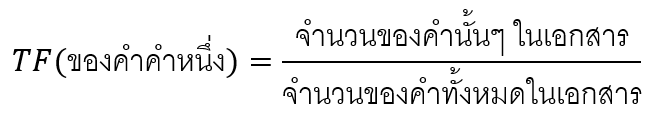
\includegraphics[width=5cm]{./figure/figure_tf.png}}
              \caption{สมการการคำนวณ Term-Frequency (TF)}\label{fig:model4}
          \end{figure}
    \item \textbf{Inverse Document Frequency (IDF)} โดยจะคำนวณความสำคัญของแต่ละคำโดยคำที่พบได้บ่อยจะมีค่า IDF ที่ต่ำ
          ซึ่งบ่งบอกว่าคำเหล่านั้นไม่สามารถดึงเอาจุดเด่นของเอกสารออกมาได้ดี
          \begin{figure}[!h]\centering
              \setlength{\fboxrule}{0.2mm} % can define this in the preamble
              \setlength{\fboxsep}{1cm}
              \fbox{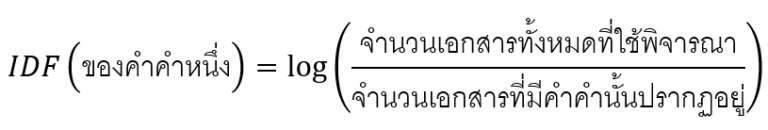
\includegraphics[width=5cm]{./figure/figure_idf.png}}
              \caption{สมการการคำนวณ Inverse Document Frequency (IDF)}\label{fig:model5}
          \end{figure}
    \item \textbf{คำนวณค่า TF-IDF} โดยเราจะนำ TF กับ IDF มาคำนวณและถ้าหากคำไหนที่มาค่า TF-IDF ที่สูง จะถูกมองว่าเป็นคำที่มีความสำคัญ
          สูง (กล่าวถึงบ่อย แต่ก็ไม่ได้ปรากฏอยู่หลายเอกสารเกินไป) และมีแนมโน้มจะเป็นใจความสำคัญของเอกสาร
          \[TFIDF = TF * IDF\]
\end{itemize}
\section{อัลกอริทึมในการแยกประเภทเรซูเม}
\subsection{อัลกอริทึม I K-Nearest Neighbors (KNN)}

% Can define this in the preamble..
เป็นอัลกอริทึมสำหรับการจัดกลุ่มข้อมูล (Classfication) ซึ่งอยู่ในกลุ่มของการเรียนรู้แบบมีผู้สอน (Supervised Learning)
หลักการทำงาน คือการจัดกลุ่มโดยอิงถึงความใกล้เคียงของข้อมูล เพื่อคาดเดาหรือจำแนกประเภทข้อมูลใหม่ \cite{kNeighbor} โดยหลักการทำงานสามารถสรุปได้ดังนี้
\begin{enumerate}
    \item  \textbf{เลือกค่า K} : กำหนดค่า K ที่ต้องการ ซึ่งเป็นจำนวนของข้อมูลที่ใกล้ที่สุดที่จะใช้ในการตัดสินใจ
    \item  \textbf{คำนวณระยะทาง} : ใช้ระยะทางยูคลิเดียน (Euclidean distance) เพื่อคำนวณหาความคล้ายคลึงระหว่างข้อมูล
    \item  \textbf{หาข้อมูลที่ใกล้ที่สุด} : หลังจากคำนวณระยะทางระหว่างข้อมูลทดสอบกับข้อมูลในชุดข้อมูลการฝึกฝน เราจะเลือกข้อมูล K รายการที่มีระยะทางน้อยที่สุด
    \item  \textbf{คำนวณผลโหวต} : เมื่อเราได้ข้อมูล K รายการที่ใกล้ที่สุดแล้ว เราจะนับจำนวนรายการในแต่ละกลุ่มหรือประเภทข้อมูล
          และกำหนดกลุ่มหรือประเภทข้อมูลของข้อมูลทดสอบตามจำนวนที่มากที่สุดใน K รายการนั้น
    \item  \textbf{ทำนายผลลัพธ์} : สุดท้ายเราก็จะได้กลุ่มข้อมูลที่ถูกแบ่งออกมาพร้อมใช้ในการทำนายต่อไป
\end{enumerate}

\begin{figure}[!h]\centering
    \setlength{\fboxrule}{0.2mm} % can define this in the preamble
    \setlength{\fboxsep}{1cm}
    \fbox{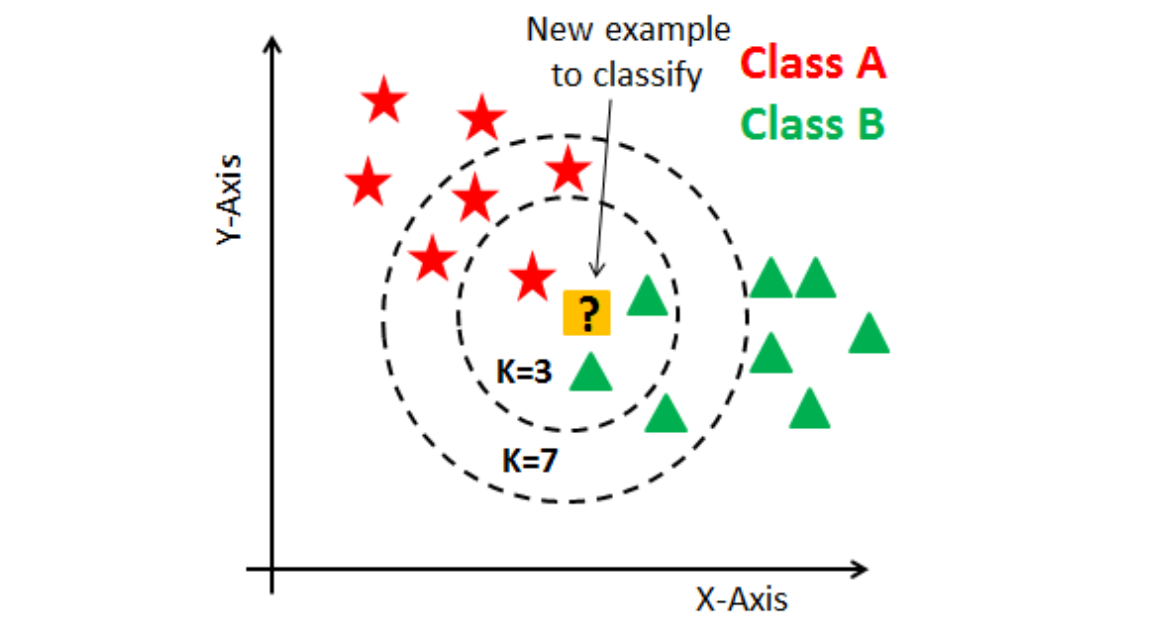
\includegraphics[width=5cm]{./figure/figure_knn.png}}
    \caption{ลักษณะการทำงานของ K-Nearest Neighbors}\label{fig:model2}
\end{figure}

\subsection{อัลกอริทึม II Naive Bayes Classifier}
Naive Bayes Classification เป็นหนึ่งใน Classification Model ใช้ในการแบ่งกลุ่มหรือหาเหตุการณ์ที่จะเกิดขึ้นโดยการอิงทฤษฎีความน่าจะเป็นของ
Bayes หรือ Bayesian
\par ซึ่งจะคำนวณว่าจะเกิดเหตุการณ์นั้นหรือไม่โดยจะเพิ่มโอกาสในการเกิดเหตุการณ์เข้าไปด้วย
โดยมักจะใช้ในการวิเคราะห์ข้อมูลที่มีความต่อเนื่องของเหตุการณ์ (Dependent Event) เช่น
โอกาสในการเกิดโรคในกลุ่มประชากรที่เราสนใจ \cite{naiveBayes-1,naiveBayes-2} ซึ่งจำเป็นจะต้องอาศัยการคำนวณผ่านสูตรดังนี้ และกำหนดให้

\begin{figure}[!h]\centering
    \setlength{\fboxrule}{0.2mm} % can define this in the preamble
    \setlength{\fboxsep}{1cm}
    \fbox{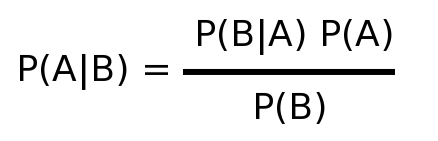
\includegraphics[width=5cm]{./figure/figure_nb.png}}
    \caption{สมการความน่าจะเป็นของ Bayes หรือ Bayesian}\label{fig:model3}
\end{figure}

\par P(A|B) คือความน่าจะเป็นในการเกิดเหตุการณ์ A โดยมี B เป็น Condition
\par P(B|A) คือความน่าจะเป็นในการเกิดเหตุการณ์ B โดยมี A เป็น Condition
\par P(A) คือโอกาสในการเกิดเหตุการณ์ A จากเหตุการณ์ทั้งหมด
\par P(B) คือโอกาสในการเกิดเหตุการณ์ B จากเหตุการณ์ทั้งหมด
\section{ภาษาคอมพิวเตอร์ และเทคโนโลยี}
\subsection{เครื่องมือในการทำโครงงาน}
\subsubsection{Figma}
\label{subsec:Figma}
เครื่องมือที่ใช้ในการออกแบบส่วนต่อประสานผู้ใช้ (User Interface) รวมถึงระดมสมอง (Brain Storm)
และใช้สำหรับให้นักออกแบบสื่อสารกับผู้อื่นให้เข้าใจได้ง่ายและเห็นภาพมากยิ่งขึ้น
เช่น การทำ User Persona, User Journey, User Flow, Site Map รวมถึงการทำ
Prototype เพื่อนำมาใช้ในการทดสอบการใช้งานของผู้ใช้ (Usability Test)
และยังสามารถออกแบบดีไซน์ของเว็บไซต์ (Design System)
เพื่อให้นักพัฒนาสามารถนำสไตล์ไปใช้พัฒนาเว็บFไซต์ได้ง่ายและเป็นระเบียบมากยิ่งขึ้น
\subsubsection{Jira}
เครื่องมือที่ช่วยในการพัฒนาซอฟต์แวร์ทางอ้อม มีส่วนช่วยในการติดตามและจัดการงานต่าง ๆ
ได้ถึงระดับย่อย เหมาะสมกับการทำงานในรูปแบบ Agile อีกทั้งยังสามารถผูกกับบริการต่าง ๆ
ภายนอกได้ ทำให้การติดตามงานสะดวกยิ่งขึ้นไปอีก
\subsection{ภาษาโปรแกรมที่ใช้}
\subsubsection{Typescript}
ภาษาที่พัฒนาต่อยอดมาจาก Javascript เพื่อปรับปรุงจุดด้อยต่าง ๆ เช่น การจัดการ
interface และประเภทของตัวแปร การเขียนโค้ดที่สนับสนุนรูปแบบ OOP ที่ดีกว่า
การตรวจจับข้อผิดพลาดและการรับมือที่ดีกว่า โดยทางเราจะนำมาใช้งานกับ framework
ต่าง ๆ ที่กล่าวไปข้างต้น เพื่อให้การทำงานมีประสิทธิภาพสูงสุด
\subsubsection{Python}
ภาษาโปรแกรมที่ถูดจัดอยู่ในประเภทระดับสูง ซึ่งถูกนำมาใช้อย่างแพร่หลายในปัจจุบัน
มีลักษณะไวยากรณ์ไม่ซับซ้อน สามารถใช้พัฒนาเว็บแอปพลิเคชัน
รวมถึงนำไปประยุกต์พัฒนาปัญญาประดิษฐ์ได้หลายประเภท
มีไลบรารี่จำนวนมาก อีกทั้งยังชุมชนใหญ่ ซึ่งในที่นี้ เราจะนำมาใช้สำหรับการพัฒนาปัญญาประดิษฐ์ของเรา
\subsection{เทคโนโลยีจัดการระบบหน้าบ้าน (Front-End)}
\subsubsection{NextJS}
React framework ซึ่งสามารถใช้สร้าง full-stack web applications ได้
แต่ทางเราจะมุ่งเน้นไปที่การนำมาใช้พัฒนาส่วน frontend โดย NextJS
จะมีความสามารถในการเขียนส่วนปฏิสัมพันธ์กับผู้ใช้ในเชิง components
เหมือนกับ React และมีส่วนเสริมต่าง ๆ เพื่อให้การทำงานของเราเป็นไปอย่าง
มีประสิทธิภาพมากขึ้น เช่น routing, caching , optimizing, configuration
ต่าง ๆ
\subsection{เทคโนโลยีจัดการระบบหลังบ้าน (Back-End)}
\subsubsection{NestJS}
Framework ที่ใช้สำหรับพัฒนาระบบ backend ซึ่งเขียนด้วยภาษา TypeScript
โดยมีพื้นหลังของการพัฒนา framework มาจาก Express และ Fastify
โดยมุ่งเน้นให้นักพัฒนาสามารถพัฒนาระบบ backend ได้อย่างรวดเร็ว
และสนับสนุนหลักการทำงานต่าง ๆ ที่นักพัฒนานิยมใช้งาน
โดยทางเราเองก็จะใช้ความสามารถในส่วนนี้เพื่อนำมาใช้พัฒนาเช่นกัน อาทิ REST API
และ MVC structure
\subsection{บริการคลาวด์ (Cloud Service)}
\subsubsection{Google Cloud Platform (GCP)}
บริการในรูปแบบ cloud ของทาง Google ซึ่งประกอบด้วยบริการหลากหลายรูปแบบ
โดยทางเรามุ่งเน้นที่จะใช้งานบริการส่วนของการหลัก ๆ ดังนี้
\begin{itemize}
    \item \textbf{Cloud Run} : บริการสำหรับการนำ container ที่มีมารันบน cloud โดยเราจะนำบริการนี้มา host ทั้งในส่วนของหน้าบ้านและหลังบ้านของเว็บแอป
    \item \textbf{Cloud Build} : บริการสำหรับนำไฟล์โปรเจ็กต์มา build ให้อยู่ในรูปแบบ container โดยเราจะนำมาใช้คู่กับ docker เพื่อนำโปรเจ็กส่งสู่ Cloud Run
    \item \textbf{Cloud Storage} : บริการสำหรับเก็บไฟล์มีเดียต่าง ๆ เช่น รูปภาพ เสียง วิดีโอ เพื่อนำมาเก็บข้อมูลของผู้ใช้ที่เป็นมีเดีย
    \item \textbf{Artifact Registry} : บริการสำหรับเก็บไฟล์ container ต่าง ๆ ที่มีทั้งหมด โดยนำมาใช้คู่กับ Cloud Build เพื่อเก็บ container ที่ผ่านการ build เสร็จแล้ว
\end{itemize}

\subsection{ระบบฐานข้อมูล}
\subsubsection{MongoDB}
Open-source database ประเภท NoSQL ที่มีโครงสร้างแบบ document
ซึ่งได้รับความนิยมอย่างสูงเนื่องจากยืดหยุ่นและปรับขนาดได้ง่าย
อีกทั้งยังรอบภาษาที่หลากหลายทั้ง Javascript, Python, Java และอื่น ๆ
โดยทางเราเลือกใช้งาน MongoDB เพราะมีเงื่อนไขที่ยืดหยุ่นเหมาะกับการทำงานของเรา
เช่น ไม่จำกัดจำนวนคำขอ API ต่อวัน และมีพื้นที่จัดเก็บที่พอเหมาะอยู่ที่ 512 GB
ในระดับการใช้งานฟรี
\subsection{เครื่องมือช่วยเหลือการพัฒนา (CI/CD Management)}
\subsubsection{Docker}
เครื่องมือที่สามารถช่วยจำลองสภาพแวดล้อมของเซิร์ฟเวอร์ด้วยหลักการ container
และ images ทำให้ขจัดปัญหาละเอียดอ่อน เช่น ปัญหาสภาพแวดล้อมในแต่ละเครื่องไม่เหมือนกันส่งผลให้รันไม่ได้ โดยเราจะนำ docker มาใช้เป็นส่วนช่วยเหลือในการนำบริการไปปล่อยสู่สาธารณะผ่าน Google Cloud
\subsubsection{Github}
ระบบควบคุมเวอร์ชัน สามารถสร้างจุด commit เพื่อเสมือนเป็นจุดบันทึกเวอร์ชันหนึ่ง
และสามารถนำไปเก็บบนที่เก็บรวม (repository) เพื่อควบคุมเวอร์ชันของไฟล์งาน
กับบุคคลภายในทีมได้ โดยทางเราจะนำมาใช้เพื่อควบคุมเวอร์ชันของซอฟต์แวร์โครงงาน
เพื่อให้ทำงานได้อย่างลื่นไหล เช่น การแยกสาขาของงานตามฟีเจอร์
การติดตามเวอร์ชันของโค้ดเพื่อค้นหาจุดกำเนิดของข้อผิดพลาดอีกทั้งยังระบุบุคคล
ผู้รับผิดชอบการทำงานส่วนนั้นได้อีกด้วย
\section{การศึกษาข้อมูลผลิตภัณฑ์ที่ใกล้เคียง}
\subsection{หนังสือหลักสูตรวิศวกรรมศาสตร์บัณฑิต สาขาวิศวกรรมคอมพิวเตอร์ มจธ.}
เป็นหนังสือที่บอกถึงรายละเอียดของแต่ละรายวิชาที่นักศึกษาวิศวกรรมคอมพิวเตอร์ได้เรียนในหลักสูตรตั้งแต่ปี 1 ถึงปี 4
โดยจะแสดงออกมาเป็นผลลัพธ์การเรียนรู้และทักษะที่ได้จากการเรียนในวิชาต่าง ๆ แต่จะไม่ได้บอกถึงอาชีพสามารถนำไปต่อยอดจากรายวิชาได้
\par ซึ่งทางคณะผู้จัดจะนำข้อมูลรายวิชาในแต่ละปีการศึกษามาศึกษามาแบ่งว่า แต่ละรายวิชาสามารถนำไปต่อยอดทางใดได้บ้าง
เพื่อมาวางแผนเส้นทางการลงวิชาเลือกที่สัมพันธ์กับระดับการศึกษาและความสนใจของผู้ใช้งานแต่ละคน

\subsection{LinkedIn}
LinkedIn เป็นเว็บแอปพลิเคชันชุมชนในสายอาชีพต่าง ๆ ที่ช่วยให้ผู้ใช้สร้างโปรไฟล์อาชีพของตนเองและเชื่อมโยงกับคนที่ใกล้เคียงในสายอาชีพ
เว็บไซต์นี้จะช่วยให้ผู้ใช้สามารถสร้างเครือข่ายในสายอาชีพของตน แบ่งปันข้อมูลเกี่ยวกับประสบการณ์การทำงาน ประวัติการศึกษา ทักษะ ความถนัด
รวมถึงเผยแพร่เนื้อหาที่เกี่ยวข้องกับสาขาอาชีพของพวกเขาในรูปแบบข่าวสาร ทำให้เชื่อมโยงและแลกเปลี่ยนข้อมูลกับผู้ใช้อื่น ๆ ในวงการได้ตลอดเวลา \\
โดยที่เว็บไซต์มีฟังก์ชันหลายอย่าง ประกอบด้วย :
\begin{itemize}
    \item \textbf{โปรไฟล์ผู้ใช้} : ผู้ใช้สามารถสร้างโปรไฟล์ส่วนตัวที่แสดงประสบการณ์การทำงาน การศึกษา ทักษะ และข้อมูลอื่นๆ เพื่อให้ผู้ใช้อื่นสามารถทราบรายละเอียดเบื้องต้นของพวกเขาได้
    \item \textbf{การเชื่อมโยง} : ผู้ใช้สามารถเชื่อมโยงกับคนอื่นในสายอาชีพ ทำให้สร้างเป็นเครือข่ายในสายอาชีพที่แข็งแกร่งขึ้น และเป็นโอกาสที่ดีให้กับผู้ใช้งานได้
    \item \textbf{โพสต์และเนื้อหา} : ผู้ใช้สามารถโพสต์เนื้อหาเกี่ยวกับวงการอาชีพ เช่น บทความ ข่าวสาร และความคิดเห็น ซึ่งช่วยในการแบ่งปันความรู้และประสบการณ์
    \item \textbf{ค้นหางาน} : ผู้ใช้สามารถค้นหางานและสมัครงานได้โดยตรงผ่านแพลตฟอร์ม และผู้ประกาศงานก็สามารถค้นหาผู้สมัครที่เหมาะสมกับตำแหน่งงานที่ว่างอยู่ของตนเองได้โดยง่าย
    \item \textbf{กลุ่มองค์กร} : บริษัทและองค์กรสามารถสร้างหรือเข้าร่วมกลุ่มบน LinkedIn เพื่อแบ่งปันข้อมูลและความรู้ในหมวดหมู่ที่เกี่ยวข้องได้ภายในกลุ่มที่กำหนดเองได้
    \item \textbf{การแสดงความสนใจ} : ผู้ใช้สามารถกดถูกใจ แสดงความคิดเห็น หรือแชร์เนื้อหาของผู้อื่น เพื่อแสดงความรับรู้ สนใจ หรือช่วยในการประกาศข่าวสารที่ดี
\end{itemize}
\par ซึ่งถือว่าเป็นเว็บแอปพลิเคชันที่เกี่ยวข้องกับการหางานที่มีความสามารถที่สูง และเน้นไปที่การสร้างคอมมูนิตี้สำหรับการทำงาน เนื่องด้วยคุณสมบัติที่หลากหลายนี้
ทำให้มีผู้ใช้งานเป็นจำนวนมาก ซึ่งทางคณะผู้จัดทำจะนำระบบชุมชนที่สามารถแนะนำงานกับกิจกรรม และระบบจัดเก็บเรซูเมมาต่อยอดกับโครงงานของเราให้ดียิ่งขึ้น

\subsection{JobDB}
เป็นเว็บแอปพลิเคชันที่รวบรวมตำแหน่งงานต่าง ๆ ในประเทศไทยที่กำลังเปิดรับอยู่ ที่จัดทำขึ้นมาสำหรับผู้คนที่กำลังมองหางาน \\
โดยที่เว็บไซต์มีฟังก์ชันหลายอย่าง ประกอบด้วย :
\begin{itemize}
    \item ระบบค้นหาอาชีพที่ต้องการ
    \item โพสต์ที่จะมีรายละเอียดงานที่เปิดรับ
    \item ระบบสมัครงาน
    \item คำแนะนำสำหรับการจัดทำเอกสารการสมัครงาน
    \item การแจ้งเตือนสำหรับตำแหน่งงานที่ผู้ใช้งานสนใจ
\end{itemize}
\par ซึ่งเป็นเว็บแอปพลิเคชันรวบรวมตำแหน่งงานที่เน้นกลุ่มเป้าหมายเป็นผู้ที่กำลังหางานในประเทศไทย โดยรวมมีระบบที่คอยอำนวยความสะดวกในการค้นหางานที่ผู้ใช้งานสนใจ
และยังมีฟังก์ชันที่น่าสนใจเป็นอย่างมากกับ ระบบคำแนะนำสำหรับการจัดทำเอกสารการสมัครงาน ซึ่งทางผู้จัดทำโครงงานจะนำฟังก์ชันนี้มาต่อยอดกับโครงงานต่อไป

\subsection{JobThai}
เป็นเว็บแอปพลิเคชันสมัครงานที่มีกลุ่มเป้าหมายเป็นคนที่กำลังมองหางานในประเทศไทย ครอบคลุมหลากหลายอาชีพ \\
โดยที่เว็บไซต์มีฟังก์ชันหลายอย่าง ประกอบด้วย :
\begin{itemize}
    \item \textbf{ระบบสมัครสมาชิก} : โดยมีทั้งฝั่งของผู้ที่กำลังหางาน และผู้ที่กำลังต้องการลูกจ้าง ซึ่งแต่ละฝ่ายก็จะมีฟังก์ชันที่รองรับ เช่น ผู้ที่กำลังหางานก็จะสามารถฝากประวัติได้
    \item \textbf{ระบบค้นหางาน} : โดยสามารถคัดกรองได้ด้วยอาชีพที่ต้องการ สถานที่ทำงาน บริษัทที่เปิดรับ ประเภทของธุรกิจ รวมไปถึงเงินเดือนอีกด้วย
    \item \textbf{โพสต์} : ที่จะมีรายละเอียดงานที่เปิดรับ
\end{itemize}
\par ซึ่งเว็บแอปพลิเคชันนี้จะเน้นไปที่ผู้ใช้งานที่อยู่ในประเทศไทย และยังมีฟังก์ชันเลือกสถานที่ทำงานที่อยู่ใกล้กับสถานีรถไฟฟ้า นิคมอุตสาหกรรม หรือแม้กระทั่งใกล้กับรถเมล์
ซึ่งถือว่าทำมาเพื่อตอบสนองกับความต้องการของผู้ใช้งานในกรุงเทพที่ดีมาก ๆ เพราะการเดินทางก็ถือเป็นหนึ่งในปัจจัยสำคัญในการเลือกงานในปัจจุบัน

\subsection{Workday}
เป็นเว็บแอปพลิเคชันที่มุ่งเน้นไปในการจัดการทรัพยากรบุคคล โดยที่ถูกออกแบบมาเพื่อรองรับการทำงานสำหรับองค์กรขนาดกลาง จนถึงองค์กรขนาดใหญ่ \\
โดยที่เว็บไซต์มีฟังก์ชันหลายอย่าง ประกอบด้วย :
\begin{itemize}
    \item \textbf{การจัดการข้อมูลพนักงาน} : รวมถึงการจัดการการสร้าง แก้ไข และยุติข้อมูลการทำงานของพนักงาน เช่น ข้อมูลส่วนตัว การจ้างงาน การเลื่อนตำแหน่ง การลางาน เป็นต้น
    \item \textbf{การจัดการงบประมาณ} : การคำนวณเงินเดือน การจ่ายเงินเดือน และการจัดการสวัสดิการสำหรับพนักงาน เช่น ประกันสุขภาพ กองทุนสำรองเลี้ยงชีพ เป็นต้น
    \item \textbf{การวางแผนแบบครบวงจร} : ตั้งแต่ขั้นตอนการรับสมัครงาน การบรรจุงาน การพัฒนาพนักงาน และการเลื่อนขั้น
\end{itemize}
\par ซึ่งเว็บแอปพลิเคชันนี้จะเน้นไปที่การให้บริการเกี่ยวกับการดูแลข้อมูลของพนักงาน ที่มีระบบที่น่าสนใจอย่างการวางแผนพัฒนาพนักงาน
รวมถึงการเลื่อนขั้น ที่ทางคณะผู้จัดทำจะนำมันมาพัฒนาต่อยอดกับการพัฒนาผู้ใช้งานที่เป็นนักศึกษาวิศวกรรมคอมพิวเตอร์ต่อไป

\subsection{Fuel50}
เป็นเว็บแอปพลิเคชันที่มีฟังก์ชัน Career Journey ที่จะให้ผู้ใช้งานสามารถกำหนดตำแหน่งงานในปัจจุบัน และตำแหน่งงานในอนาคตที่ต้องการจะเป็น
ซึ่งตัวเว็บไซต์จะมีระบบแนะนำตั้งแต่ตำแหน่งที่จำเป็นต้องเป็นก่อนจะถึงจุดหมาย รวมไปถึงทักษะที่ต้องพัฒนา
และทักษะที่จำเป็นต้องเพิ่มเพื่อที่จะสามารถพัฒนาตำแหน่งงานไปได้อย่างมีประสิทธิภาพ
\par ซึ่งนักศึกษามองว่าฟังก์ชัน Career Journey นี้จะมีประโยชน์อย่างมากสำหรับนักศึกษาวิศวกรรมคอมพิวเตอร์ที่เป็นผู้ใช้งานของเรา
ทางคณะผู้จัดทำจึงอยากที่จะนำมาปรับปรุงและแก้ไขเพื่อมาใช้กับแนวทางการเลือกวิชา (Class Journey) เพื่อให้ผู้ใช้งานเห็นภาพการพัฒนาตนเองที่ชัดเจนยิ่งขึ้น
และทำให้ผู้ใช้งานมีแรงจูงใจในการพัฒนาตนเองต่อไป

\subsection{Super Resume}
ซุปเปอร์เรซูเม (Super Resume) คือ แพลตฟอร์มสร้างเรซูเมออนไลน์ที่มีผู้ใช้งานมากกว่า 2 ล้านคนในประเทศไทย
รูปแบบของซุปเปอร์เรซูเมได้รับการพัฒนาโดยบริษัทชั้นนำและได้รับการยอมรับจาก HR ของบริษัทชั้นนำกว่า 30,000 บริษัท ซุปเปอร์เรซูเมมีรูปแบบที่เป็นมาตรฐานและครบถ้วน
ครอบคลุมข้อมูลสำคัญของผู้สมัครงาน ได้แก่ ข้อมูลส่วนตัว ข้อมูลการศึกษา ข้อมูลประสบการณ์การทำงาน ข้อมูลทักษะและความสามารถ และข้อมูลความถนัดและบุคลิกภาพ \\
ข้อดีของการใช้ซุปเปอร์เรซูเมในการสมัครงาน ประกอบด้วย :
\begin{itemize}
    \item HR ที่คุ้นเคยกับรูปแบบของซุปเปอร์เรซูเมจะทำให้สามารถอ่านและเข้าใจข้อมูลของผู้สมัครได้อย่างรวดเร็วและง่ายดาย
    \item ซุปเปอร์เรซูเมมีข้อมูลที่ครบถ้วนและครอบคลุม ทำให้ผู้สมัครสามารถนำเสนอข้อมูลของตนเองได้อย่างมีประสิทธิภาพ
    \item ซุปเปอร์เรซูเมสามารถจัดส่งไปยังบริษัทที่ตรงกับความต้องการของผู้สมัครได้โดยตรง
    \item ซุปเปอร์เรซูเมยังมีฟังก์ชันที่ช่วยให้ผู้สมัครสามารถติดตามสถานะการสมัครงานและปรับปรุงเรซูเมของตนเองได้อีกด้วย
\end{itemize}
\par โดยสรุป ซุปเปอร์เรซูเมเป็นแพลตฟอร์มสร้างเรซูเมออนไลน์ที่มีประสิทธิภาพและช่วยให้ผู้สมัครงานมีโอกาสในการสมัครงานและสัมภาษณ์งานมากขึ้น
ซึ่งคณะผู้จัดทำได้เล็งเห็นว่าการสร้างเรซูเมเป็นสิ่งที่สำคัญมาก จึงอยากที่จะมีระบบที่ให้คำแนะนำเกี่ยวกับเรซูเมขึ้นมาในโครงงานของเรา
เพื่อที่ผู้ใช้งานจะสามารถทราบได้ว่าควรที่จะเพิ่มเติมรายละเอียดของเรซูเมอย่างไรบ้าง

\subsection{JobHack (Resume Checker)}
เป็นเว็บแอปพลิเคชันสำหรับการตรวจสอบคุณภาพเรซูเม ว่ามีความเหมาะสมกับตำแหน่งที่ผู้ใช้งานกำลังสนใจหรือไม่ โดยจะให้คะแนนออกมา
และยังแนะนำส่วนที่ขาดหายอีกทั้งยังมีแนวคำถามที่ผู้สัมภาษณ์อาจจะถามอีกด้วย
\par ซึ่งนักศึกษามองว่าการนำ Artificial Intelligence มาตรวจสอบคุณภาพของเรซูเมเป็นฟังก์ชันที่น่าสนใจเป็นอย่างมาก แต่ทาง JobHack
ยังคงมีความแม่นยำที่น้อย ซึ่งทางคณะผู้จัดทำมองว่าเป็นสิ่งที่ดีหากสามารถนำมาพัฒนาต่อให้มีประสิทธิภาพมากยิ่งขึ้น

\subsection{Competitor Analysis}
\begin{table}[!h]
    \caption{ตารางเปรียบเทียบคุณสมบัติที่สนใจ}\label{tbl:method1}
    \begin{tabular}{c|c|c|c} \hline
                     & การทำนายเรซูเม & รายละเอียดเชิงลึกของสายอาชีพ & แผนภาพสายอาชีพ \\ \hline
        * Compath    & \checkmark   & \checkmark               & \checkmark    \\ \hline
        LinkedIn     &              &                          &               \\ \hline
        JobDB        &              & \checkmark               &               \\ \hline
        JobThai      &              & \checkmark               &               \\ \hline
        Workday      &              & \checkmark               &               \\ \hline
        Fuel50       &              & \checkmark               & \checkmark    \\ \hline
        Super Resume &              & \checkmark               &               \\ \hline
        JobHack      & \checkmark   & \checkmark               &               \\ \hline
    \end{tabular}
\end{table}

%%%%%%%%%%%%%%%%%%%%%%%%%%%%%%%%%%%%%%%%%%%%%%%%%%%%%55
%%%%%%%%%%%%%%%%%%%%%%%%%%%%%%%%%%%%%%%%%%%%%%%%%%%%%
%%%%%%%%%%%%%%%%%%%%%%%%%%%%%%%%%%%%%%%%%%%%%%%%%%%%%

\chapter{การออกแบบและวิธีการดำเนินงาน}

\section{การสำรวจความต้องการกับผู้ใช้}
ทางคณะผู้จัดทำได้ทำออกเก็บข้อมูลกับกลุ่มเป้าหมายมาแล้วทั้งหมด 4 ครั้ง โดยแบ่งเป็นการสัมภาษณ์เชิงปริมาณหนึ่งครั้งและเชิงคุณภาพสามครั้ง  โดยมีจุดประสงค์ในแต่ละการสัมภาษณ์ต่างกันเพื่อพิสูจน์ความต้องการของกลุ่มเป้าหมายจนกระทั่งโครงงานของเราได้ปรับตามความต้องการนั้นจนเป็นโครงงานในปัจจุบัน อย่างไรก็ตาม เรายังได้รับข้อมูลที่น่าสนใจเพิ่มเติมโดยสรุป ดังนี้

\subsection{การสัมภาษณ์เชิงปริมาณผ่านแบบสำรวจ}
ทางคณะผู้จัดทำได้ทำแบบสอบถามเพื่อหาอัตราส่วนของพฤติกรรมที่น่าสนใจ โดยได้รับข้อมูลที่สำน่าสนใจดังนี้
\begin{figure}[!h]\centering
    \setlength{\fboxrule}{0.2mm} % can define this in the preamble
    \setlength{\fboxsep}{0.5cm}
    \fbox{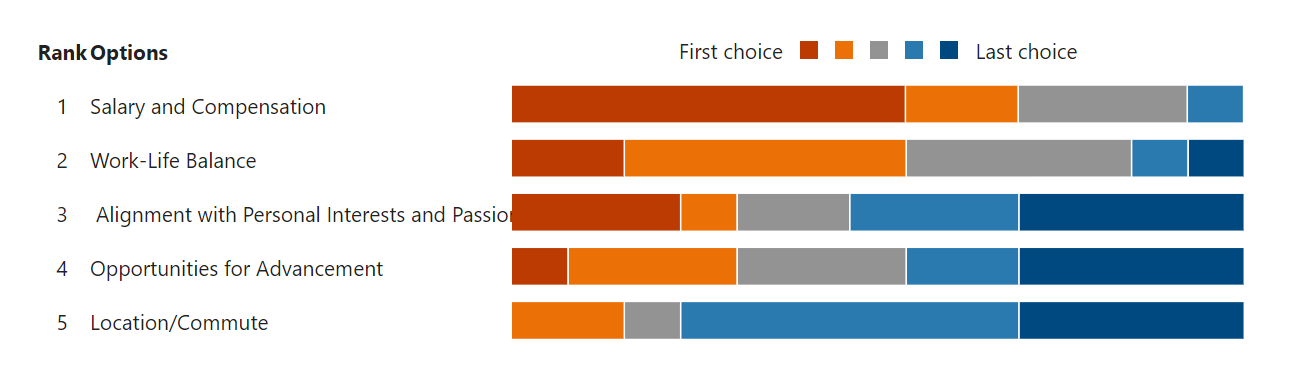
\includegraphics[width=10cm]{./figure/figure_poll.png}}
    \caption{ข้อมูลจากแบบสำรวจเชิงปริมาณ}\label{fig:insightPoll}
\end{figure}
จากข้อมูลในแบบสำรวจข้อนี้ ทำให้ทราบว่าปัจจัยที่มีผลต่อการเลือกสายงานในการทำงานมากสำหรับกลุ่มตัวอย่างก็คือเงินเดือน และความสมดุลของการทำงานกับชีวิตส่วนตัว กล่าวคือกลุ่มตัวอย่างให้ความสำคัญกับความจริงมากยิ่งขึ้น ความมั่นคง หรือเงินเดือนที่สามารถทำให้ดำเนินชีวิตได้อย่างราบรื่น รวมถึงการแบ่งเวลา การพักผ่อนที่เหมาะสมกับการทำงาน โดยมองอาจจะไม่ได้ให้ความสำคัญกับความชื่นชอบมากขนาดนั้น

\subsection{การสัมภาษณ์เชิงคุณภาพผ่านการสัมภาษณ์ตัวต่อตัว}
ทางคณะผู้จัดทำได้ออกสัมภาษณ์กับกลุ่มเป้าหมายแบบตัวต่อตัว และในการสัมภาษณ์แต่ละครั้ง จะสัมภาษณ์ที่จำนวนราว 5 คน ตามหลักการ 5 Users design โดยได้รับข้อมูลที่น่าสนใจในแต่ละครั้งมาดังนี้
\newline
\textbf{การสัมภาษณ์เชิงคุณภาพครั้งที่ 1}
\newline
\textbf{จุดประสงค์: เพื่อค้นหารากขอปัญหาที่แท้จริงของกลุ่มเป้าหมาย}
\newline
\textbf{ข้อมูลสำคัญ: }
\begin{itemize}
    \item กลุ่มเป้าหมายค้นพบความต้องการของตนเองมาจากการได้ลงมือทำจริงเป็นหลัก
    \item ส่วนใหญ่แล้วจะได้ลงมือทำจริงตอนโปรเจ็กต์วิชาเรียนหรือฝึกงาน ซึ่งอยู่ชั้นปีที่ 2 เป็นต้นไปแล้ว
    \item อยากรู้ก่อนเป็นอย่างมาก ว่าในการทำงานจริงต้องมีความสามารถอะไรบ้าง ใช้เครื่องมืออะไร
    \item กลุ่มเป้าหมายรู้สึกว่าอาจรู้ตัวช้าเกินไป หากมีโอกาสพัฒนาตนเองได้เร็วกว่านี้จะดีมาก
\end{itemize}


\noindent\textbf{การสัมภาษณ์เชิงคุณภาพครั้งที่ 2}
\newline
\textbf{จุดประสงค์: เพื่อพิสูจน์ความมีคุณภาพของวิธีการแก้ปัญหาที่ออกแบบ}
\newline
\textbf{ข้อมูลสำคัญ: }
\begin{itemize}
    \item กลุ่มเป้าหมายอยากได้ตัวช่วยในการทำให้ตนเองสมัครงานได้ง่ายขึ้น โดยหลังการทดลองถามความเห็น พบว่าสิ่งที่ต้องการเป็นหลักคือ การตรวจสอบและยืนยันได้ ว่าเรซูเม่ของตนเองเหมาะสมกับอาชีพที่ตนเองสนใจขนาดไหนแล้ว
    \item กลุ่มเป้าหมายรู้สึกสนใจในฟีเจอร์ช่วยเหลือการค้นหาแหล่งพัฒนาตนเอง เพราะเคยรู้สึกว่าตนเองอาจเริ่มพัฒนาช้าเกินไป เพราะรู้ใจตัวเองในช่วงที่อาจเรียนอยู่ชั้นปีที่ 2-3 แล้ว
    \item การตัดสินใจลงวิชาเรียนค่อนข้างมีจุดขัดใจ เพราะไม่ค่อยมีรีวิวหรือความเห็นของผู้ที่เคยเรียน ถึงแม้เคยมีแหล่งชุมชนที่รุ่นพี่เคยมอบให้ แต่รีวิวส่วนใหญ่จะมีความเก่าแล้ว ทำให้ใช้อ้างอิงได้ยาก
\end{itemize}


\noindent\textbf{การสัมภาษณ์เชิงคุณภาพครั้งที่ 3}
\newline
\textbf{จุดประสงค์: เพื่อทดลองนำ prototype ของเว็บแอปไปพิสูจน์ความรู้สึกในการใช้งานกับผู้ใช้}
\newline
\textbf{ข้อมูลสำคัญ:}
\begin{itemize}
    \item ผู้ใช้ไม่มีปัญหากับการกรอกข้อมูลเรซูเมเพื่อวิเคราะห์ แต่หากมีระบบที่กรอกข้อมูลให้อัตโนมัติผ่านไฟล์ pdf ก็ถือว่าเป็นเรื่องดี
    \item การมีระบบโหวตวิชาที่อยากให้เปิด อาจไม่ได้เป็นการการันตีว่าจะเปิดได้จริง อาจไม่สำคัญมากนัก
    \item ในอนาคต หากมีระบบที่เป็นตัวช่วยในการสร้างเรซูเมจากข้อมูลที่มีได้ ก็จะเป็นเรื่องที่ดีเช่นกัน
    \item ควรมีการแบ่ง tag ประเภทของชุมชนเพื่อความสะดวกในการค้นหา
\end{itemize}

\section{ความสามารถของระบบ}
\subsection{Use Case Diagram}
\begin{figure}[H]\centering
    \setlength{\fboxrule}{0.2mm} % can define this in the preamble
    \setlength{\fboxsep}{0.5cm}
    \fbox{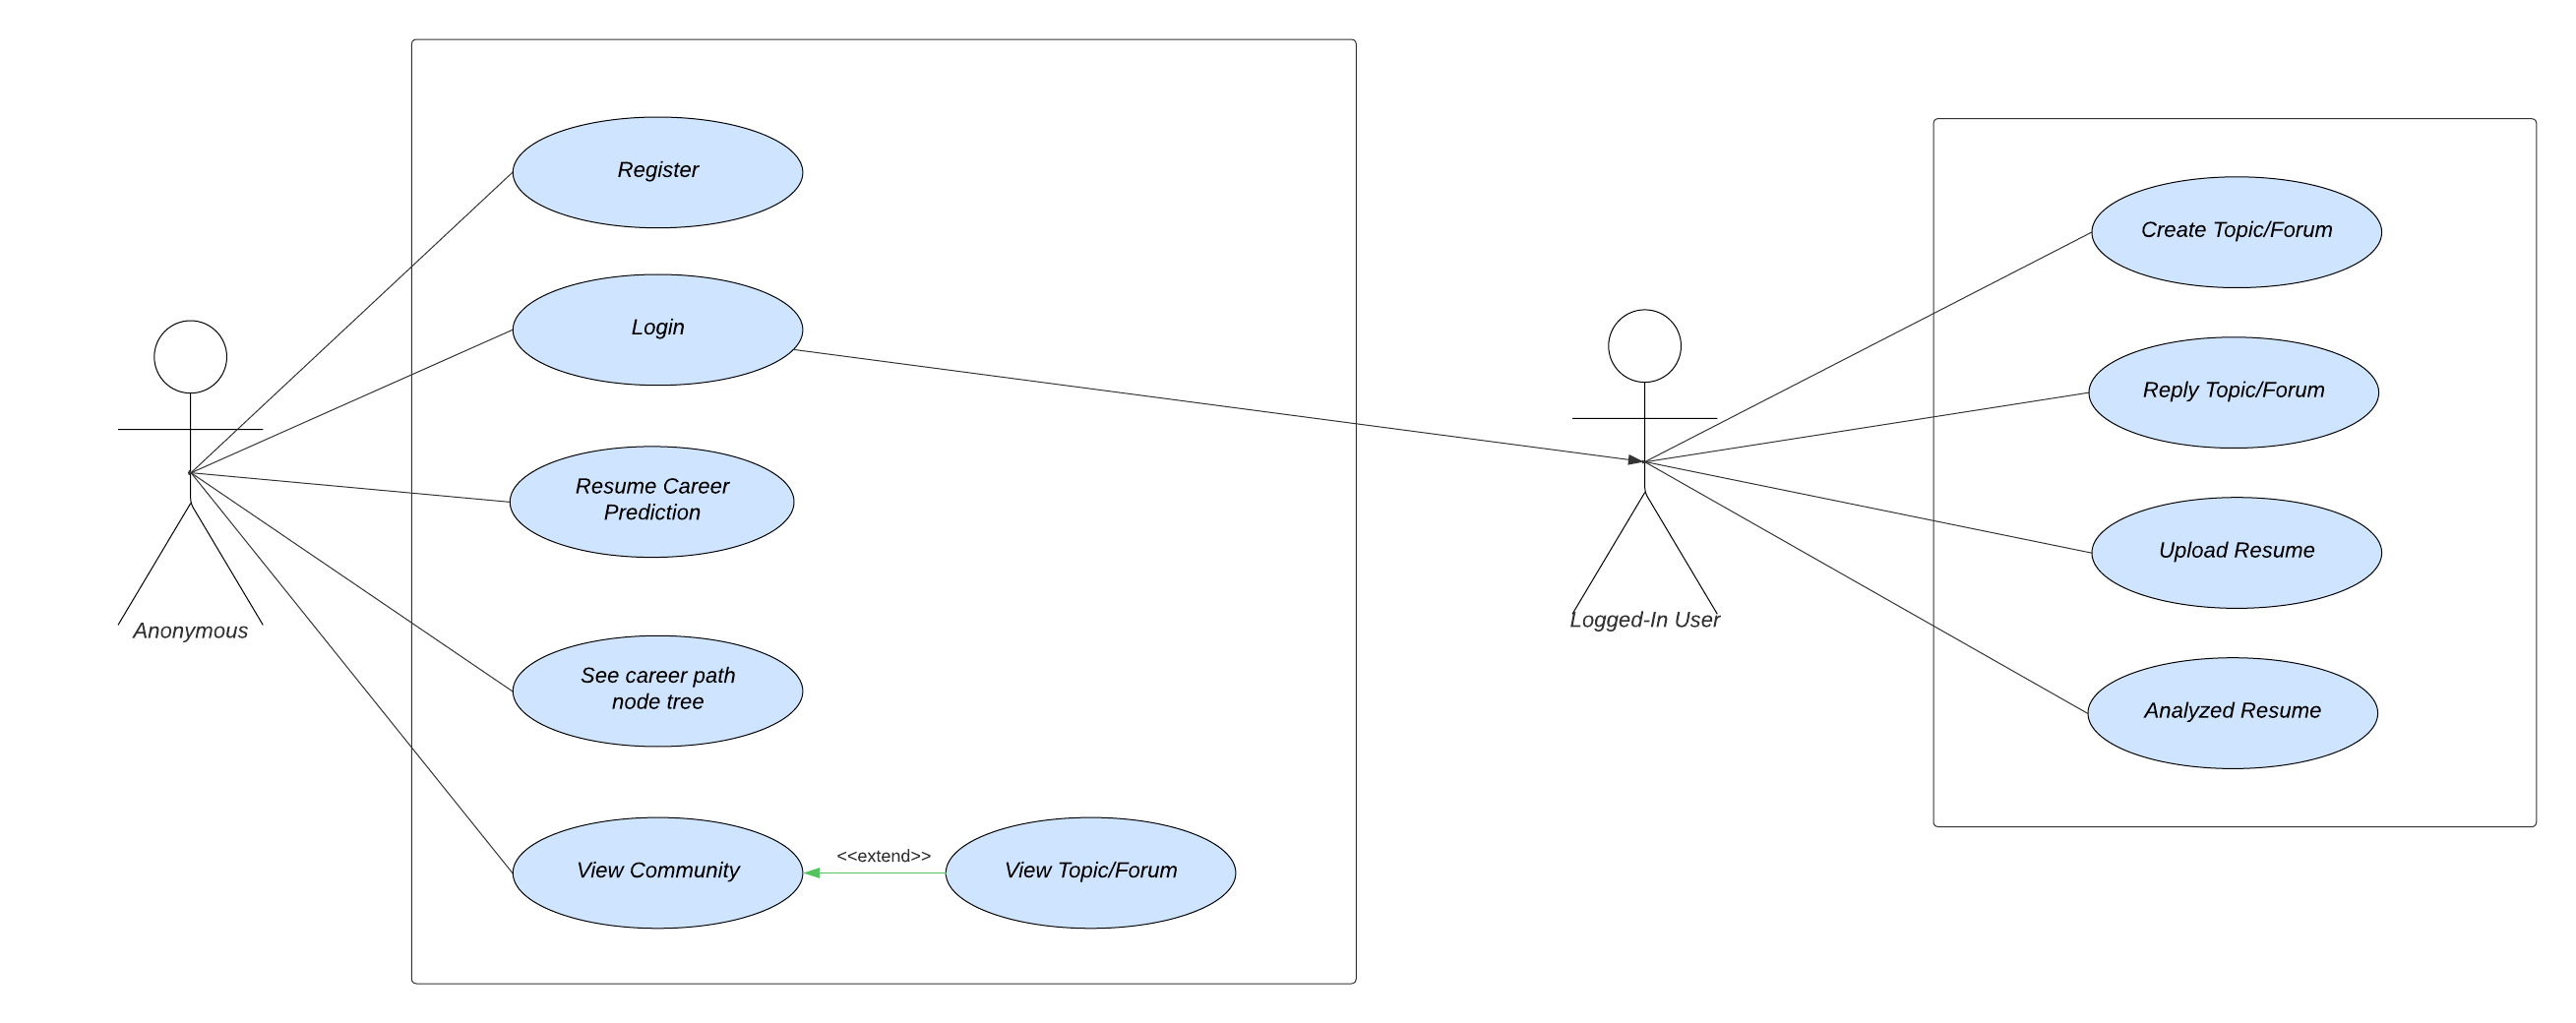
\includegraphics[width=10cm]{./figure/figure_usecase.png}}
    \caption{Use Case Diagram}\label{fig:usecase}
\end{figure}
\subsection{Use Case Narrative}
\subsubsection{Resume Career Prediction}
\begin{table}[H]
    % \centering
    \begin{tabular}{l|l} \hline
        Actor                 & Anonymous                                       \\ \hline
        Goal                  & ต้องการทราบถึงอาชีพที่เหมาะสมกับตนเอง                 \\ \hline
        Precondition          & -                                               \\ \hline
        Main success scenario & 1. ผู้ใช้ขอคำแนะนำอาชีพที่เหมาะสมกับตนเอง                \\
                              & 2. ระบบถามข้อมูลของผู้ใช้                            \\
                              & 3. ผู้ใช้กรอกข้อมูล                                  \\
                              & 4. ระบบถามเพื่อยืนยันการกรอกข้อมูล                    \\
                              & 5. ผู้ใช้ยืนยันการกรอกข้อมูล                           \\
                              & 6. ระบบแสดงอาชีพที่เหมาะสมกับผู้ใช้                    \\ \hline
        Extensions (a)        & 5a. ผู้ใช้กรอกข้อมูลไม่ครบ                            \\
                              & 6a. ระบบขึ้นเตือนว่าผู้ใช้ยังกรอกข้อมูลไม่ครบ              \\
                              & 7a. กลับไปที่ขั้นตอนที่ 3                              \\ \hline
        Postcodition          & ระบบแนะนำให้ผู้ใช้ไปวิเคราะห์ข้อมูลเชิงลึกของอาชีพที่ได้แนะนำไป \\ \hline
    \end{tabular}
\end{table}

\subsubsection{See career path node tree}
\begin{table}[H]
    % \centering
    \begin{tabular}{l|l} \hline
        Actor                 & Anonymous                                              \\ \hline
        Goal                  & ต้องการดูแผนผังสายอาชีพ                                    \\ \hline
        Precondition          & ผู้ใช้กำลังดูแผนผังรวมของสายอาชีพ                              \\ \hline
        Main success scenario & 1. ใช้เลือกอาชีพที่ต้องการจะดู                                \\
                              & 2. ระบบแสดงรายละเอียดย่อยเป็นรูปแบบแผนผังของสายอาชีพที่ผู้ใช้เลือก \\ \hline
        Extensions (a)        & 1a. ผู้ใช้ยังไม่ได้เลือกอาชีพที่ต้องการจะดู                        \\
                              & 2a. ระบบขึ้นเตือนว่าผู้ใช้ยังไม่ได้เลือกอาชีพที่ต้องการดู              \\
                              & 3a. กลับไปที่ขั้นตอนที่ 1                                     \\ \hline
        Postcodition          & -                                                      \\ \hline
    \end{tabular}
\end{table}

\subsubsection{View Community}
\begin{table}[H]
    % \centering
    \begin{tabular}{l|l} \hline
        Actor                 & Anonymous                              \\ \hline
        Goal                  & ต้องการดูรายการของกระทู้ต่าง ๆ ในชุมชน       \\ \hline
        Precondition          & ผู้ใช้กำลังดูประเภทของกระทู้                   \\ \hline
        Main success scenario & 1. ผู้ใช้เลือกประเภทของกระทู้                \\
                              & 2. ระบบแสดงรายการของกระทู้ประเภทที่ผู้ใช้เลือก \\ \hline
        Extensions (a)        & -                                      \\ \hline
        Postcodition          & -                                      \\ \hline
    \end{tabular}
\end{table}

\subsubsection{View Topic/Forum}
\begin{table}[H]
    % \centering
    \begin{tabular}{l|l} \hline
        Actor                 & Anonymous                                        \\ \hline
        Goal                  & ต้องการดูรายละเอียดของกระทู้                          \\ \hline
        Precondition          & ผู้ใช้กำลังดูรายการของกระทู้ที่อยู่ในชุมชน (กระทู้ประเภทไหนก็ได้) \\ \hline
        Main success scenario & 1. ผู้ใช้เลือกกระทู้ที่ต้องการดูรายละเอียด                  \\
                              & 2. ระบบแสดงรายละเอียดของกระทู้ผู้ใช้เลือก               \\ \hline
        Extensions (a)        & -                                                \\ \hline
        Postcodition          & -                                                \\ \hline
    \end{tabular}
\end{table}

\subsubsection{Create Topic/Forum}
\begin{table}[H]
    % \centering
    \begin{tabular}{l|l} \hline
        Actor                 & Logged-in User                                   \\ \hline
        Goal                  & ต้องการสร้างกระทู้                                   \\ \hline
        Precondition          & ผู้ใช้กำลังดูรายการของกระทู้ที่อยู่ในชุมชน (กระทู้ประเภทไหนก็ได้) \\ \hline
        Main success scenario & 1. ผู้ใช้เลือกกระทู้ที่ต้องการดูรายละเอียด                  \\
                              & 2. ระบบถามรายละเอียดภายในกระทู้                     \\
                              & 3. ผู้ใช้กรอกรายอะเอียดภายในกระทู้                     \\
                              & 4. ระบบถามเพื่อยืนยันการลงกระทู้                       \\
                              & 5. ผู้ใช้ยืนยันการลงกระทู้                              \\
                              & 6. ระบบสร้างและแสดงกระทู้ของผู้ใช้                     \\ \hline
        Extensions (a)        & 5a. ผู้ใช้กรอกข้อมูลไม่ครบ                             \\
                              & 6a. ระบบขึ้นเตือนว่าผู้ใช้ยังกรอกข้อมูลไม่ครบ               \\
                              & 7a. กลับไปที่ขั้นตอนที่ 3                               \\ \hline
        Postcodition          & กระทู้ของผู้ใช้แสดงอยู่ในชุมชน                           \\ \hline
    \end{tabular}
\end{table}

\subsubsection{Reply Topic/Forum}
\begin{table}[H]
    % \centering
    \begin{tabular}{l|l} \hline
        Actor                 & Logged-in User                                   \\ \hline
        Goal                  & ต้องการแสดงความคิดเห็นในกระทู้                        \\ \hline
        Precondition          & ผู้ใช้กำลังดูรายการของกระทู้ที่อยู่ในชุมชน (กระทู้ประเภทไหนก็ได้) \\ \hline
        Main success scenario & 1. ผู้ใช้เลือกส่วนที่ต้องการแสดงความคิดเห็น                \\
                              & 2. ระบบถามถึงรายละเอียดความคิดเห็น                   \\
                              & 3. ผู้ใช้กรอกความคิดเห็น                              \\
                              & 4. ระบบถามเพื่อยืนยันการแสดงความคิดเห็น                \\
                              & 5. ผู้ใช้ยืนยันการแสดงความคิดเห็น                       \\
                              & 6. ระบบสร้างและแสดงความคิดเห็นของผู้ใช้ในกระทู้          \\ \hline
        Extensions (a)        & 4a. ผู้ใช้ยังไม่ได้กรอกความคิดเห็น                       \\
                              & 5a. ระบบขึ้นเตือนว่าผู้ใช้ยังไม่ได้กรอกความคิดเห็น           \\
                              & 6a. กลับไปที่ขั้นตอนที่ 3                               \\ \hline
        Postcodition          & ความคิดเห็นของผู้ใช้แสดงอยู่ในกระทู้                      \\ \hline
    \end{tabular}
\end{table}

\subsubsection{Upload Resume}
\begin{table}[H]
    % \centering
    \begin{tabular}{l|l} \hline
        Actor                 & Logged-in User                                  \\ \hline
        Goal                  & ต้องการอัพโหลดเรซูเม่                               \\ \hline
        Precondition          & ผู้ใช้กำลังอยู่ดูข้อมูลส่วนตัวของตนเอง                      \\ \hline
        Main success scenario & 1. ผู้ใช้เลือกเรซูเม่ที่ต้องการอัพโหลด                    \\
                              & 2. ระบบถามเพื่อยืนยันการอัพโหลดเรซูเม่                 \\
                              & 3. ผู้ใช้ยืนยันการอัพโหลดเรซูเม่                        \\
                              & 4. ระบบอัพโหลดและแจ้งเตือนว่าอัพโหลดเรซูเม่สำเร็จ        \\ \hline
        Extensions (a)        & 3a. ผู้ใช้เลือกเรซูเม่ที่ต้องการอัพโหลด                   \\
                              & 4a. ระบบขึ้นเตือนว่าผู้ใช้ยังไม่ได้เลือกเรซูเม่ที่ต้องการอัพโหลด \\
                              & 5a. กลับไปที่ขั้นตอนที่ 1                              \\ \hline
        Postcodition          & เรซูเม่แสดงอยู่ในข้อมูลส่วนตัวของผู้ใช้                    \\ \hline
    \end{tabular}
\end{table}

\subsubsection{Analyzed Resume}
\begin{table}[H]
    % \centering
    \begin{tabular}{l|l} \hline
      Actor                 & Logged-in User                  \\ \hline
      Goal                  & ต้องการดูข้อมูลเชิงลึกของอาชีพ         \\ \hline
      Precondition          & ผู้ใช้ต้องมีอาชีพที่ระบบแนะนำให้          \\ \hline
      Main success scenario & 1. ผู้ใช้เลือกอาชีพที่ต้องการดูข้อมูลเชิงลึก \\
                            & 2. ระบบแสดงข้อมูลเชิงลึกของอาชีพ     \\ \hline
      Extensions (a)        & 1a. ผู้ใช้ต้องวิเคราะห์อาชีพใหม่        \\
                            & 2a. ระบบถามถึงข้อมูลของผู้ใช้         \\
                            & 3a. ผู้ใช้กรอกข้อมูลใหม่              \\
                            & 4a. ผู้ใช้ยืนยันการกรอกข้อมูล          \\
                            & 5a. ระบบแสดงอาชีพที่เหมาะสมกับผู้ใช้   \\
                            & 6a. กลับไปที่ขั้นตอนที่ 1              \\ \hline
      Postcodition          & -                               \\ \hline
  \end{tabular}
\end{table}

\section{สถาปัตยกรรมของระบบ}
\begin{figure}[H]\centering
    \setlength{\fboxrule}{0.2mm} % can define this in the preamble
    \setlength{\fboxsep}{0.5cm}
    \fbox{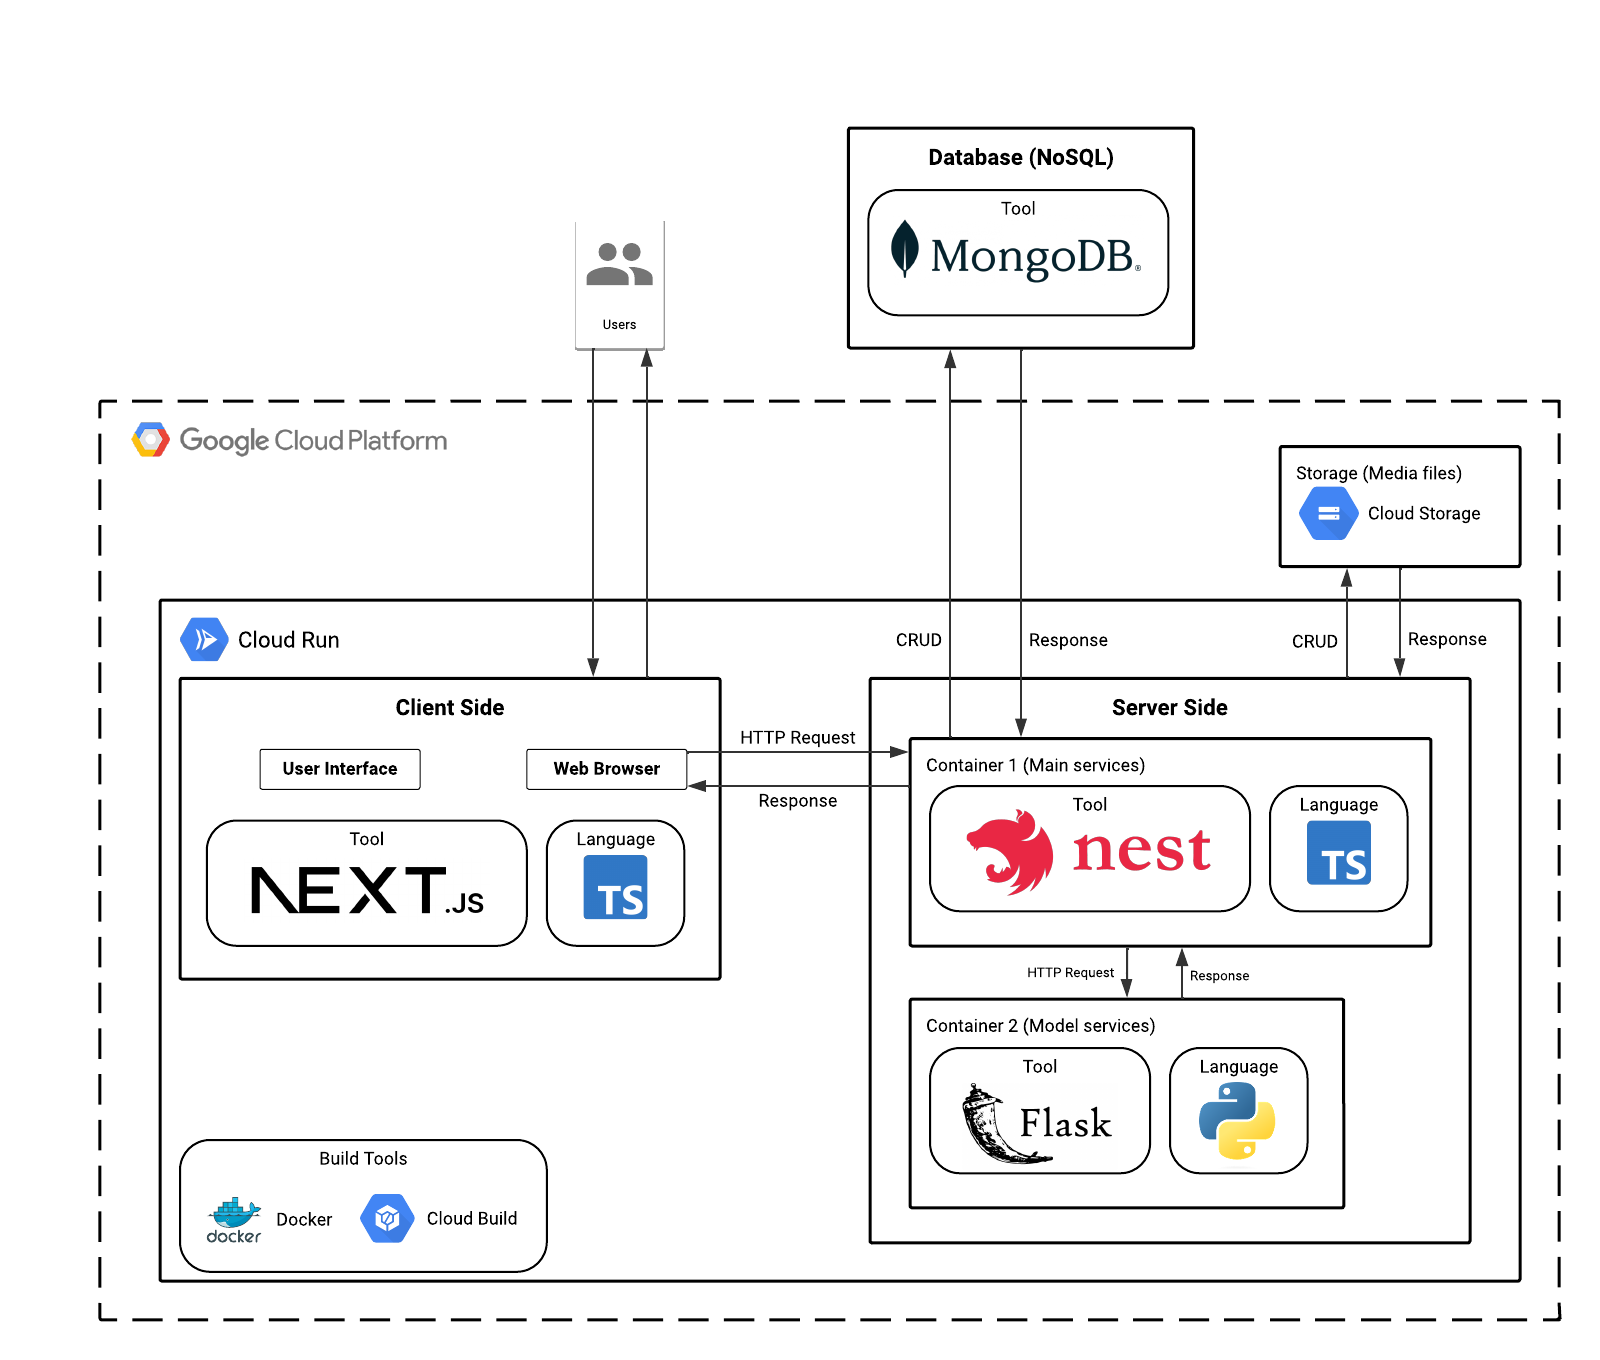
\includegraphics[width=10cm]{./figure/figure_system_architecture.png}}
    \caption{System Architecture}\label{fig:system_architecture}
\end{figure}
จากแผนผังสถาปัตยกรรมระบบ เราได้ใช้บริการ Google Cloud เป็นหลักเนื่องจากสะดวกต่อการ scaling ในอนาคต สามารถจัดการและเปลี่ยนแปลงเวอร์ชันได้รวดเร็วระหว่างการพัฒนา โดยสถาปัตยกรรมแต่ละส่วนมีหน้าที่หลักดังนี้

\subsection{ส่วนผู้ใช้ (Client-Side)}
รับผิดชอบในการติดต่อปฏิสัมพันธ์กับผู้ใช้ แสดง user interface ผ่านทาง web browser และเชื่อมต่อกับ server เพื่อขอข้อมูลและใช้บริการต่าง ๆ

\subsection{ส่วนเซิร์ฟเวอร์ (Server-Side)}
รับผิดชอบในการจัดการตรรกะและระบบคำนวณต่าง ๆ ทุกรูปแบบและส่งกลับไปให้ผู้ใช้ โดยทางคณะู้จัดทำได้แบ่งระบบ server เป็นสองบริการหลัก ประกอบด้วย
\newline
1. บริการหลัก (Main services)
\newline
บริการที่จะติดต่อกับผู้ใช้โดยตรงเพียงหนึ่งเดียว มีหน้าที่ในการจัดการทุกคำขอจากผู้ใช้ผ่านทาง API (Application Programming Interfaces) เช่น ดึงข้อมูลจากฐานข้อมูล คำนวณค่าต่าง ๆ และติดต่อกับบริการอื่น ๆ
\newline
2. บริการโมเดล (Model services)
\newline
บริการสำหรับใช้คำนวณเกี่ยวกับปัญญาประดิษฐ์ของทางคณะผู้จัดทำเท่านั้น เนื่องจากกินทรัพยากรสูง การแยกบริการออกมาจากบริการหลักจึงสามารถดูแลและจัดการได้ง่ายกว่า โดยจะรับค่ามาจากส่วนบริการหลักและส่งค่ากลับไปให้

\section{Sequence Diagram}
\subsection{Register}
\begin{figure}[H]\centering
    \setlength{\fboxrule}{0.2mm} % can define this in the preamble
    \fbox{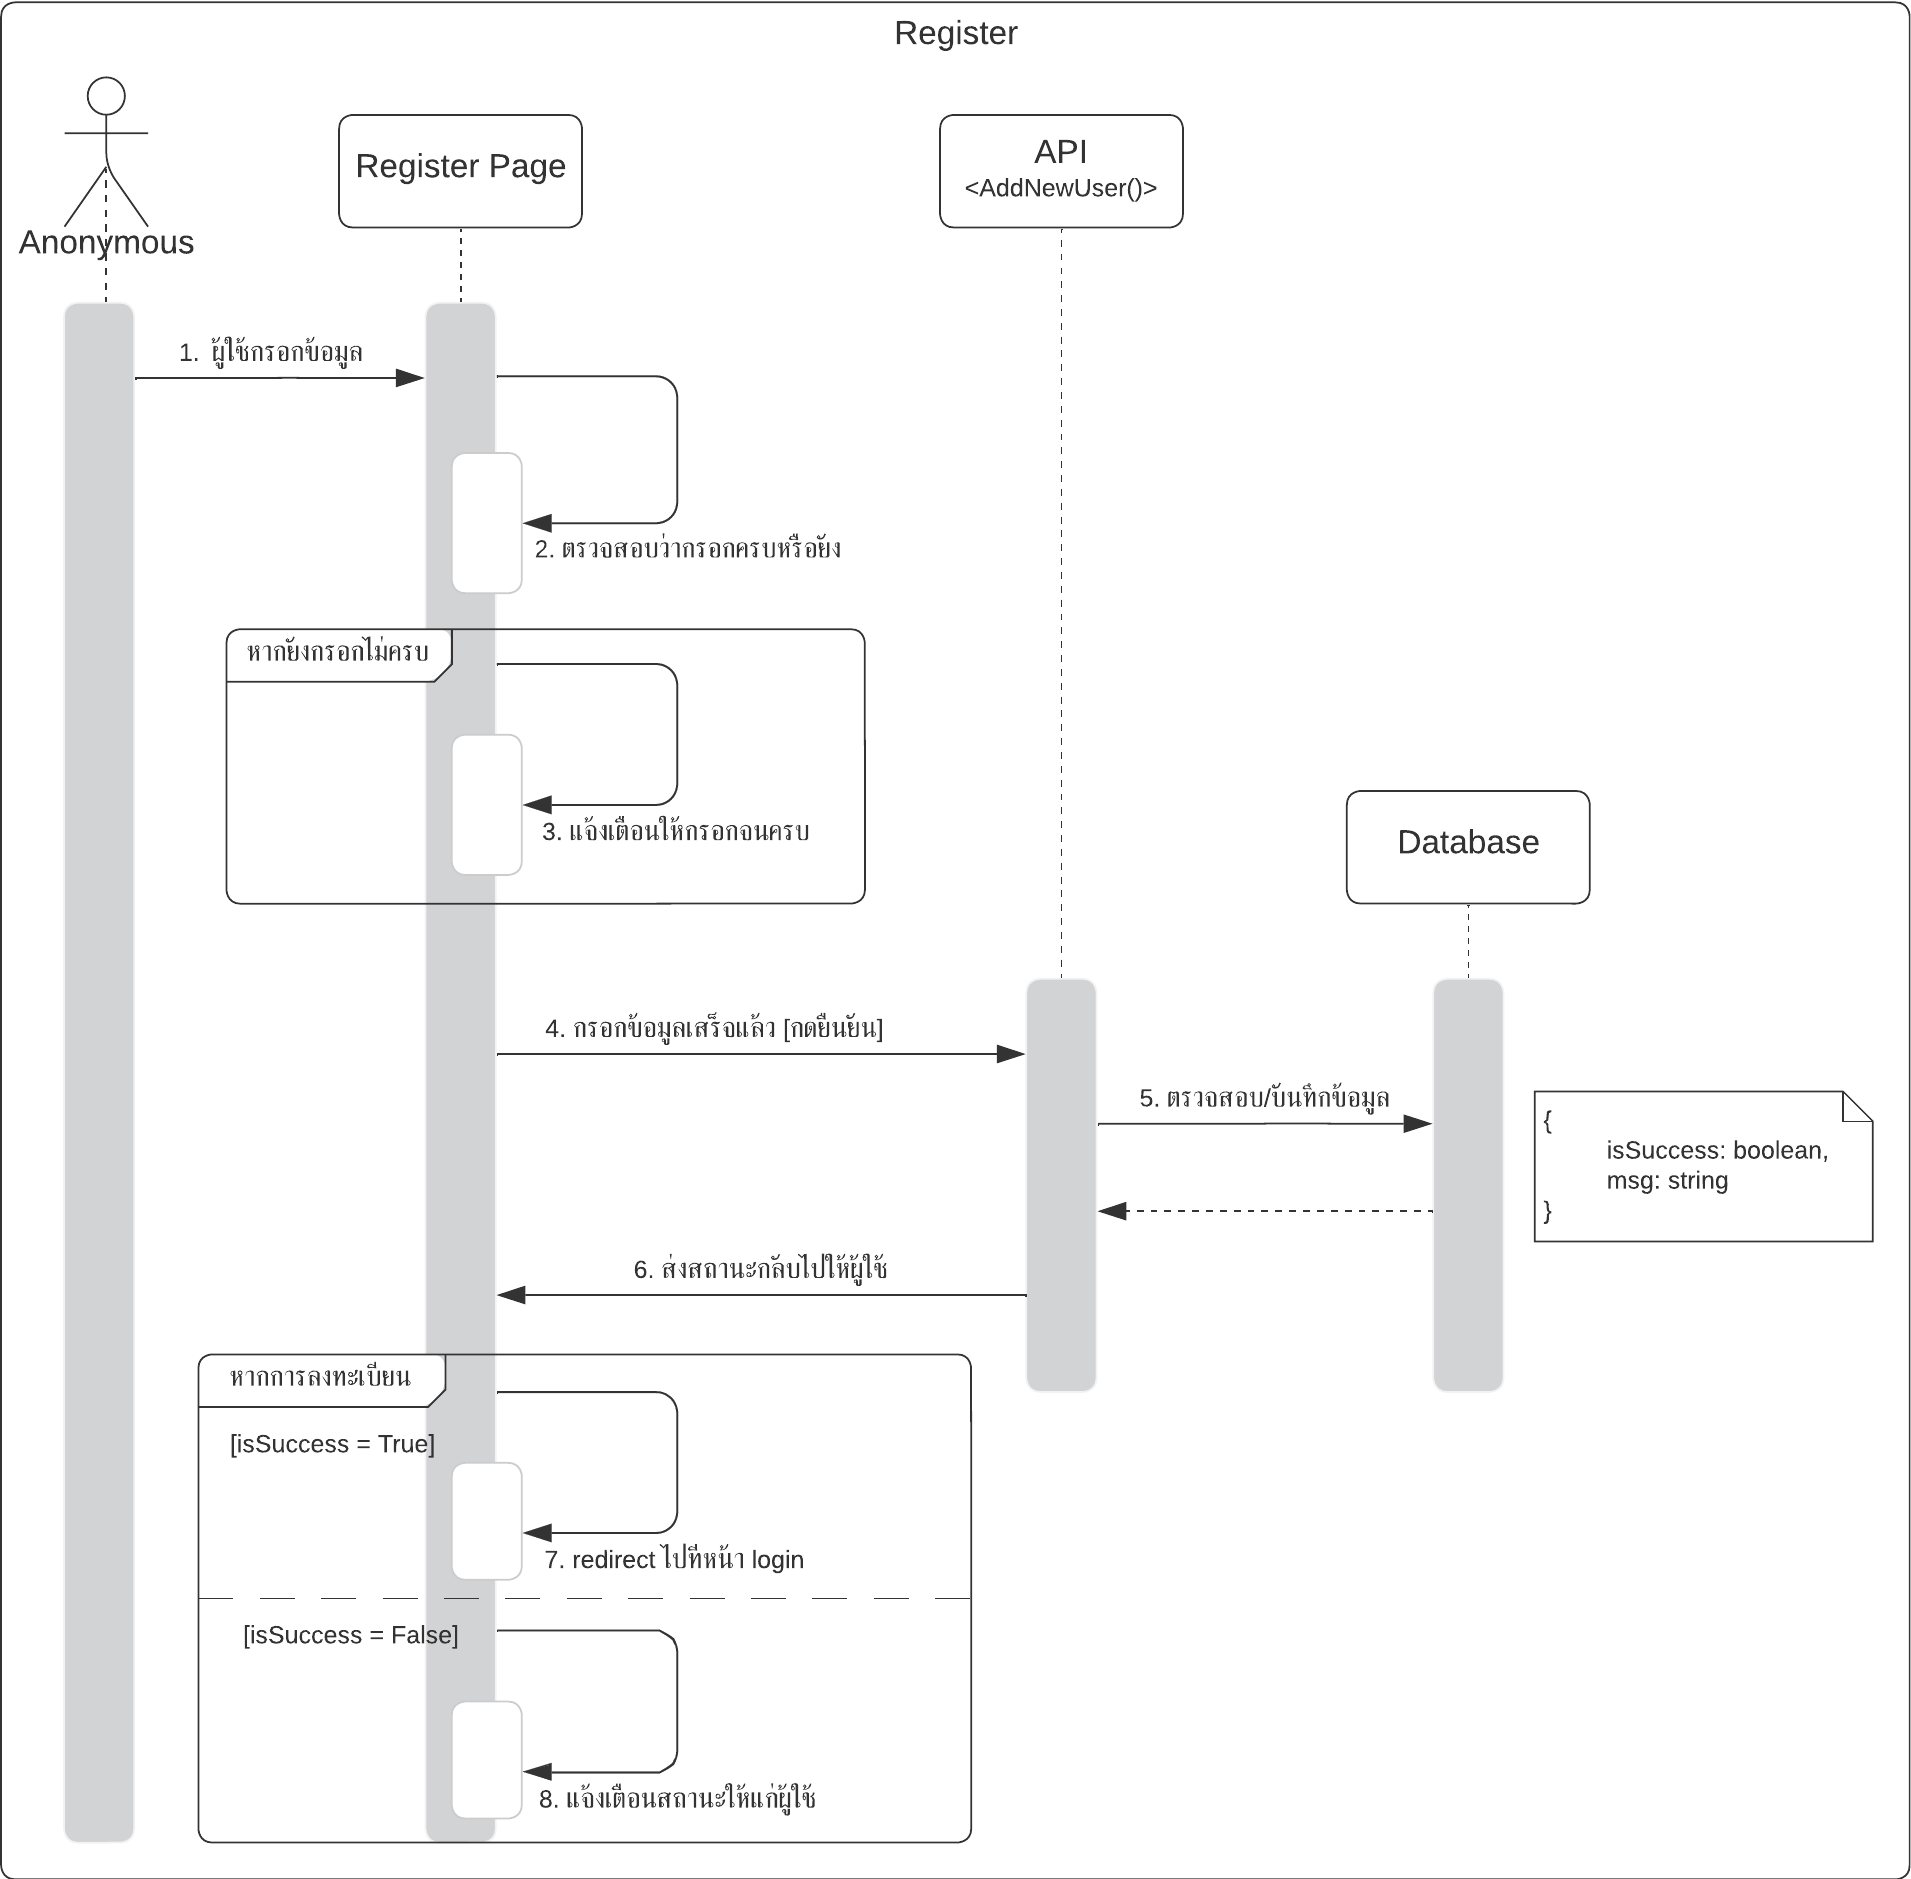
\includegraphics[width=8cm]{./figure/sequence-diagram/figure_sequence_register.png}}
    \caption{Register Sequence Diagram}\label{fig:regisSeqDiagram}
\end{figure}
\textbf{สถานการณ์: }ผู้ใช้สมัครสมาชิก
\begin{enumerate}
    \item ผู้ใช้กรอกข้อมูลในหน้าสมัครสมาชิก
    \item user interface จะทำการรับมือในกรณีที่ผู้ใช้กรอกข้อมูลยังไม่ถูกต้อง
    \item เมื่อข้อมูลถูกต้องแล้ว ผู้ใช้ทำการกดยืนยัน และส่งคำขอไปที่บริการส่วนหลัก
    \item บริการส่วนหลักทำการตรวจสอบข้อมูลผู้ใช้เดิม หากยังไม่มีข้อมูลจะบันทึกข้อมูลใหม่ลงญานข้อมูลและส่งสถานะกลับสู่ผู้ใช้ หากมีอยู่แล้วจะทำการส่งสถานะกลับสู่ผู้ใช้ทันที
    \item เมื่อผู้ใช้ได้รับสถานะ หากสำเร็จที่ส่งผู้ใช้ไปที่หน้า login หากไม่สำเร็จจะแจ้งเตือนให้แก่ผู้ใช้
\end{enumerate}

\subsection{Login}
\begin{figure}[H]\centering
    \setlength{\fboxrule}{0.2mm} % can define this in the preamble
    \fbox{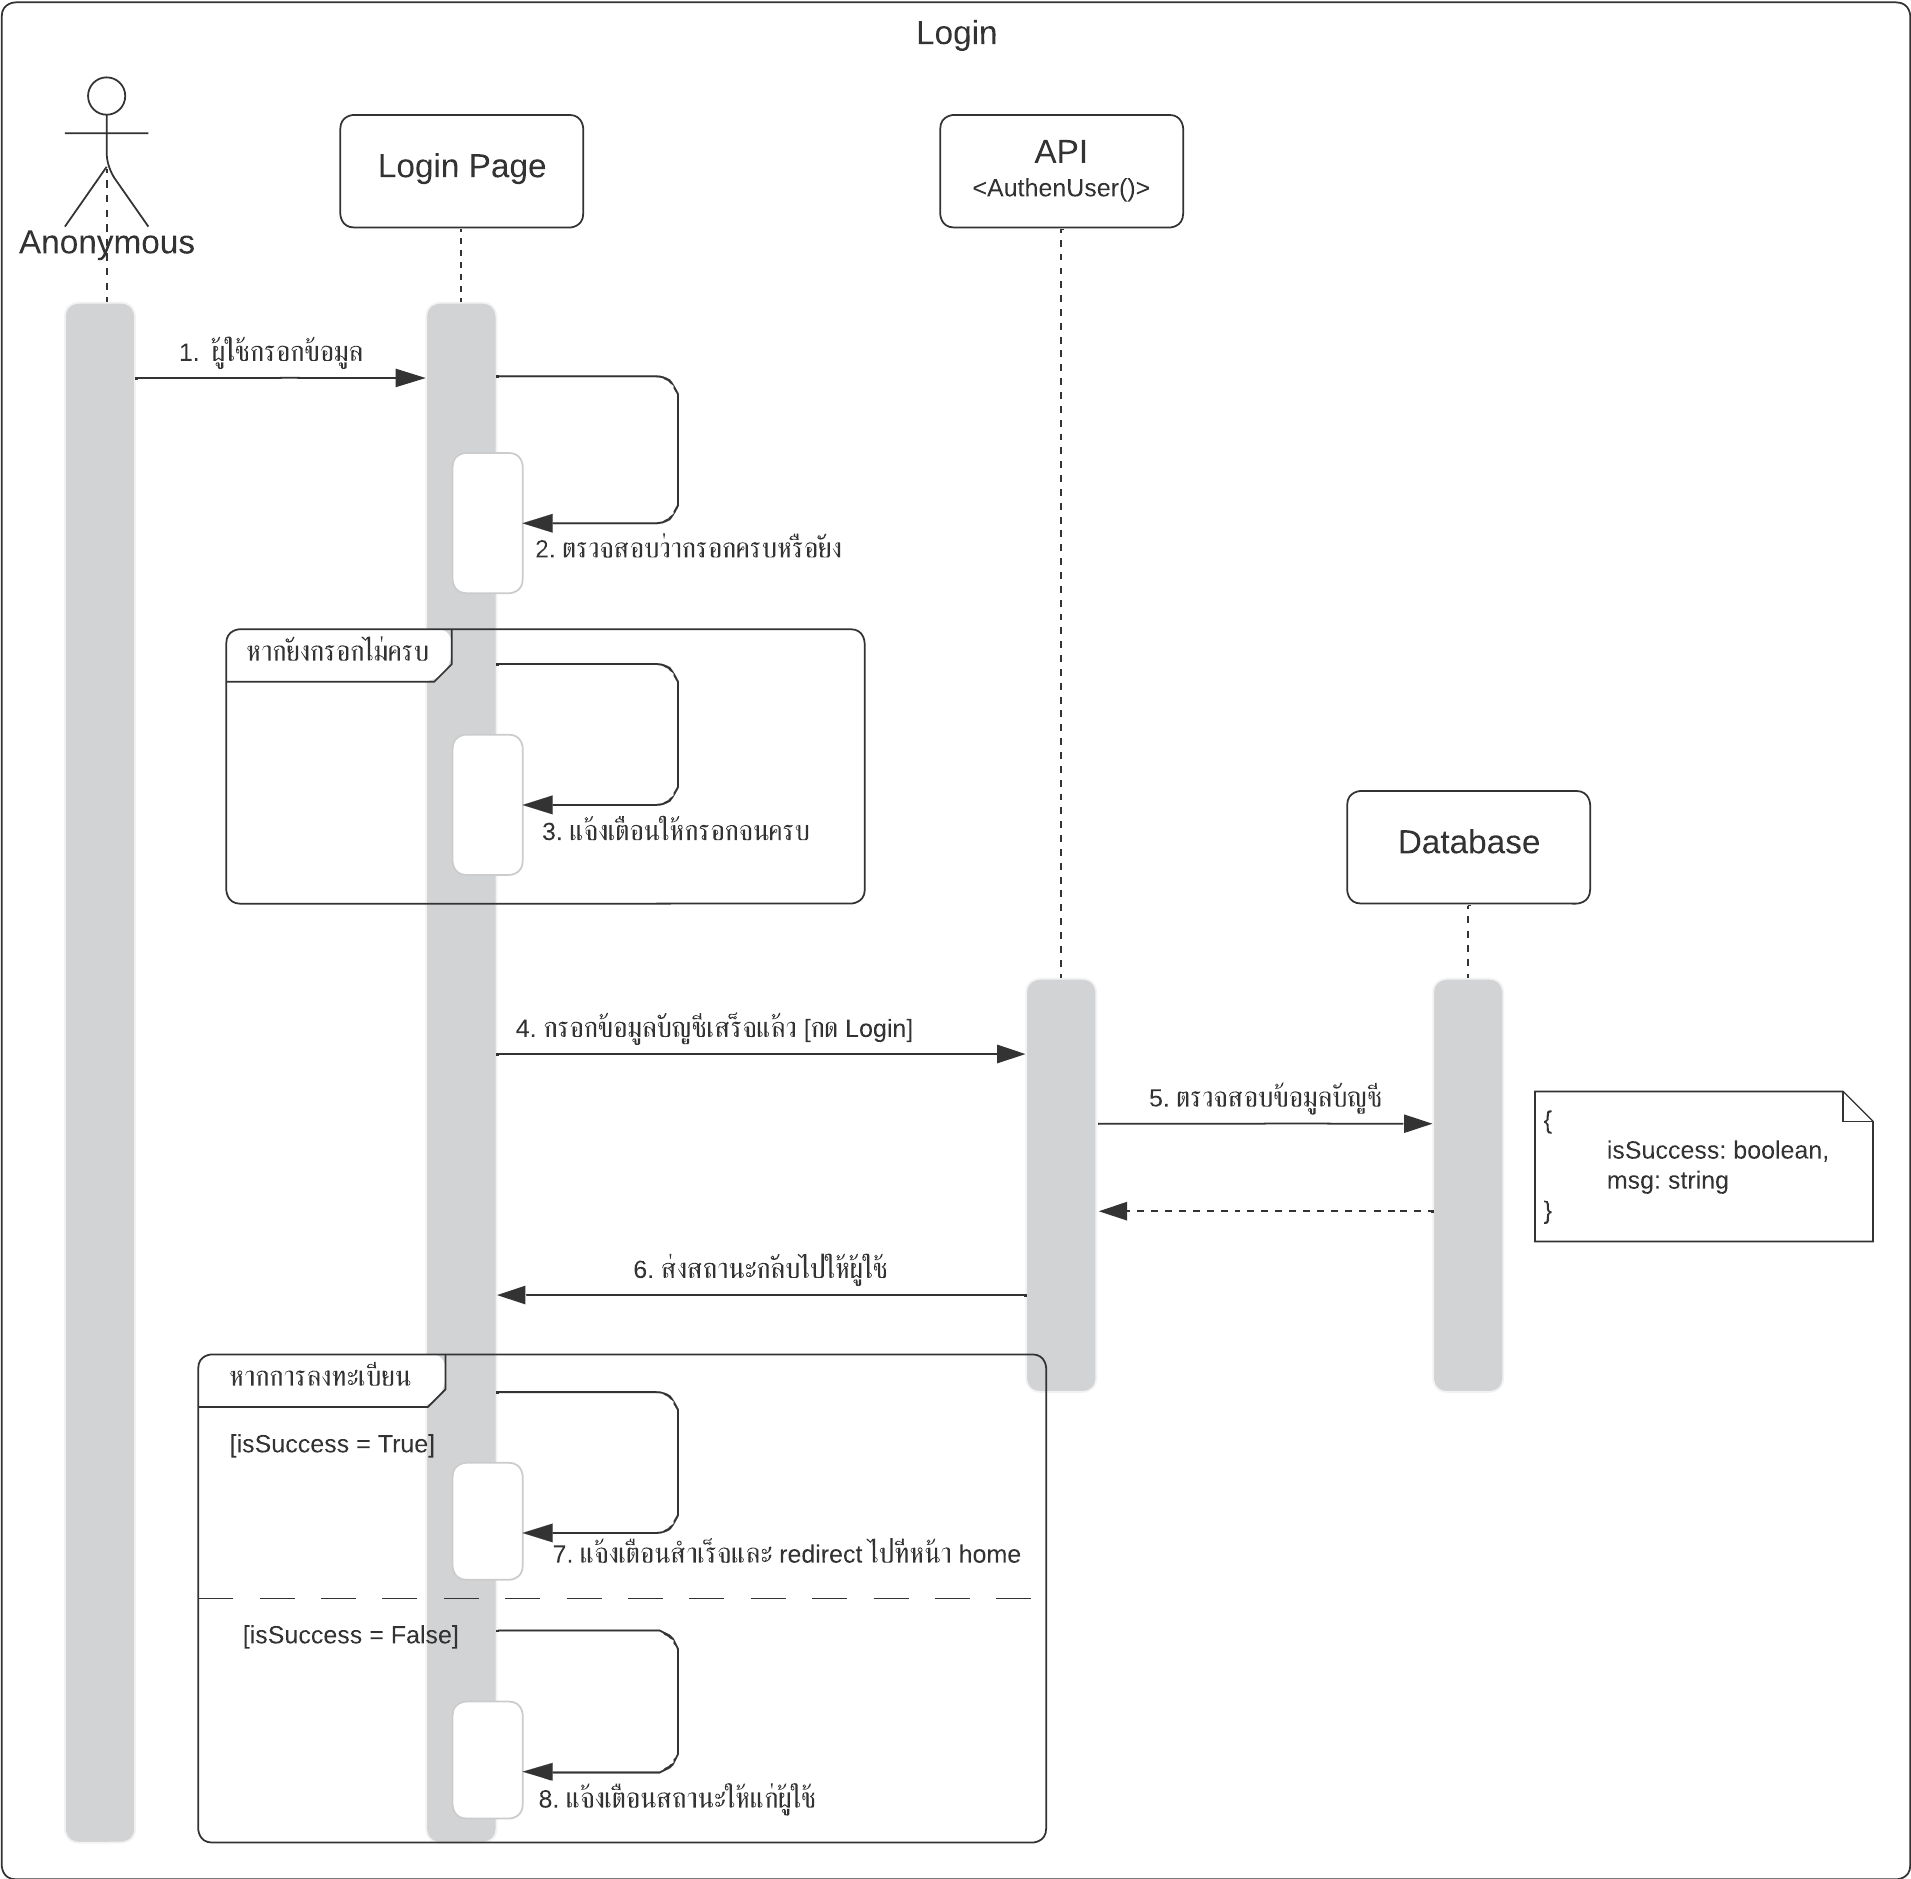
\includegraphics[width=8cm]{./figure/sequence-diagram/figure_sequence_login.png}}
    \caption{Login Sequence Diagram}\label{fig:loginSeqDiagram}
\end{figure}
\textbf{สถานการณ์: }ผู้ใช้ล็อกอิน
\begin{enumerate}
    \item ผู้ใช้กรอกข้อมูลในหน้าล็อกอิน
    \item user interface จะทำการรับมือในกรณีที่ผู้ใช้กรอกข้อมูลยังไม่ถูกต้อง
    \item เมื่อข้อมูลถูกต้องแล้ว ผู้ใช้ทำการกดยืนยัน และส่งคำขอไปที่บริการส่วนหลัก
    \item บริการส่วนหลักตรวจสอบข้อมูลผู้ใช้ที่มีอยู่ และส่งสถานะกลับสู่ผู้ใช้
    \item เมื่อผู้ใช้ได้รับสถานะ หากสำเร็จที่ส่งผู้ใช้ไปที่หน้าหลัก หากไม่สำเร็จจะแจ้งเตือนให้แก่ผู้ใช้
\end{enumerate}

\subsection{Resume Prediction}
\begin{figure}[H]\centering
    \setlength{\fboxrule}{0.2mm} % can define this in the preamble
    \fbox{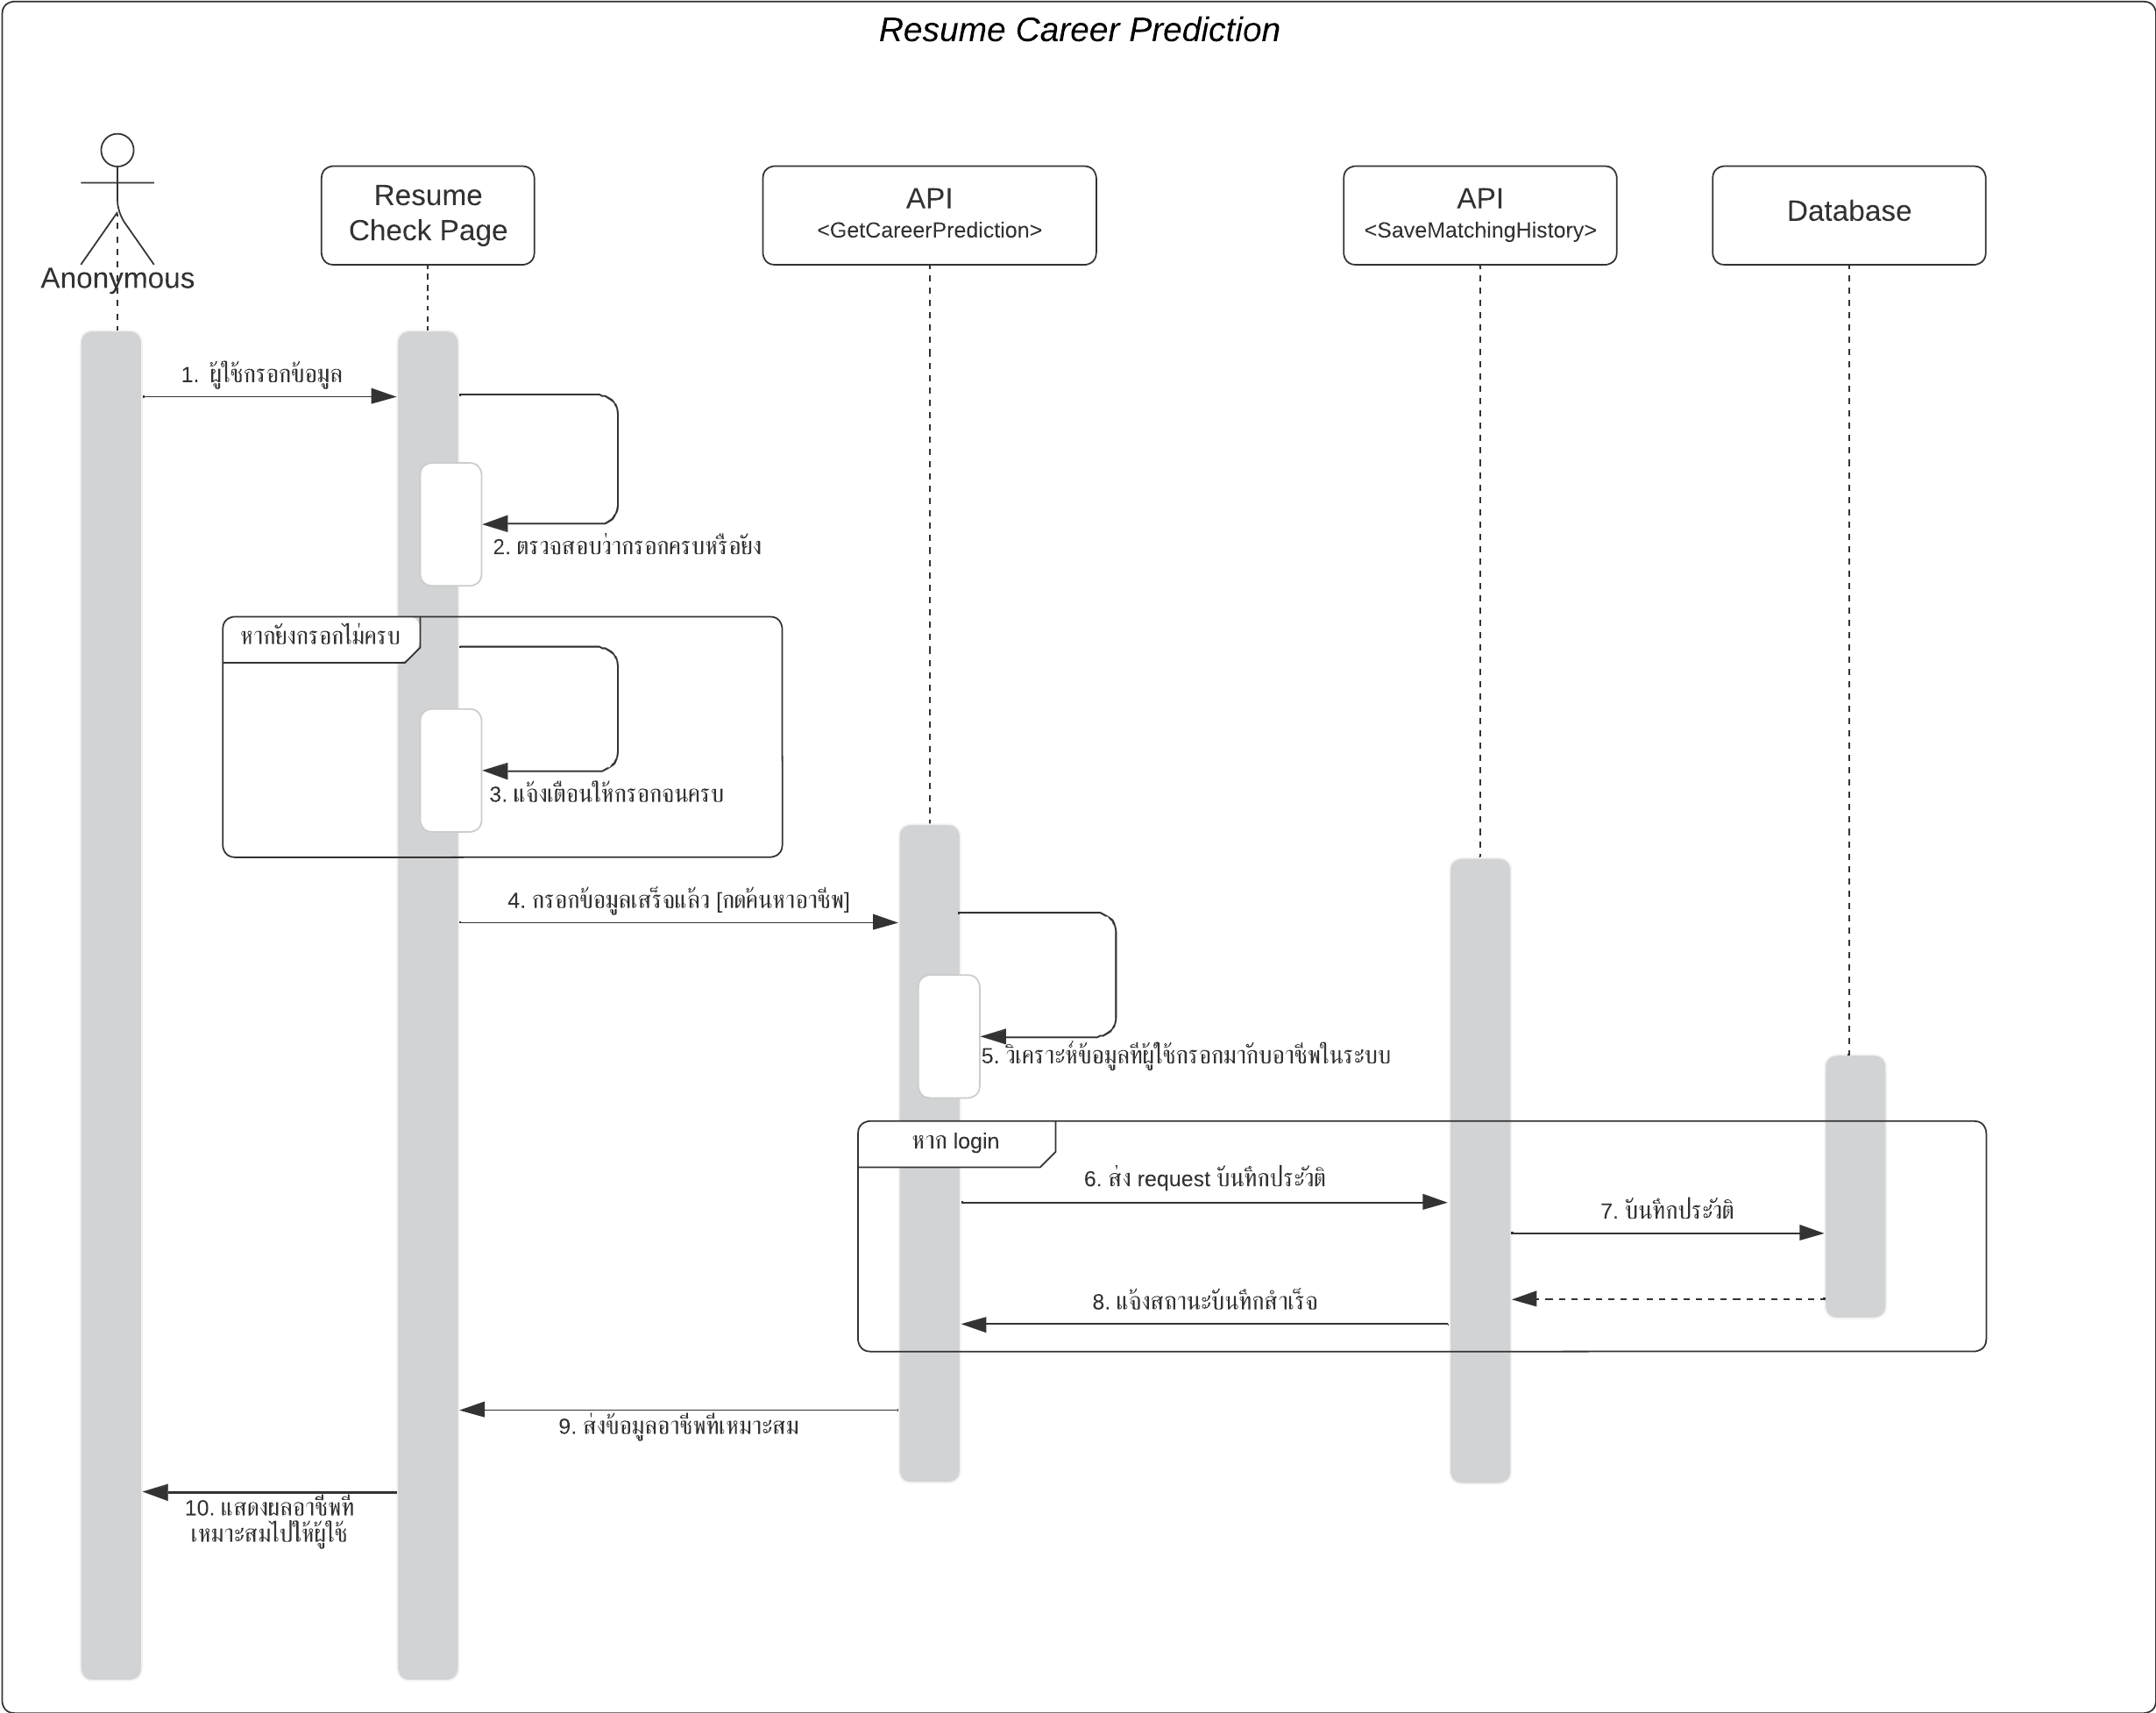
\includegraphics[width=8cm]{./figure/sequence-diagram/figure_sequence_resume_predict.png}}
    \caption{Resume Prediction Sequence Diagram}\label{fig:resumePredictSeqDiagram}
\end{figure}
\textbf{สถานการณ์: }ผู้ใช้ใช้งานระบบวิเคราะห์เรซูเม
\begin{enumerate}
    \item ผู้ใช้กรอกข้อมูลเรซูเมของตัวเอง
    \item user interface รับมือกรณีที่ผู้ใช้กรอกข้อมูลไม่ครบ และแจ้งเตือนแก่ผู้ใช้
    \item ผู้ใช้กรอกข้อมูลถูกต้องและส่งคำขอสู่บริการหลัก
    \item บริการหลักจัดการวิเคราะห์ข้อมูลเรซูเมของผู้ใช้ ในกรณีที่ผู้ใช้ login จะทำการบันทึกค่ารับเข้าต่าง ๆ ลงสู่ฐานข้อมูลเพื่อสำรองข้อมูลให้ผู้ใช้
    \item ส่งข้อมูลกลับสู่ผู้ใช้และแสดงผล
\end{enumerate}

\subsection{Analyze Resume}
\begin{figure}[H]\centering
    \setlength{\fboxrule}{0.2mm} % can define this in the preamble
    \fbox{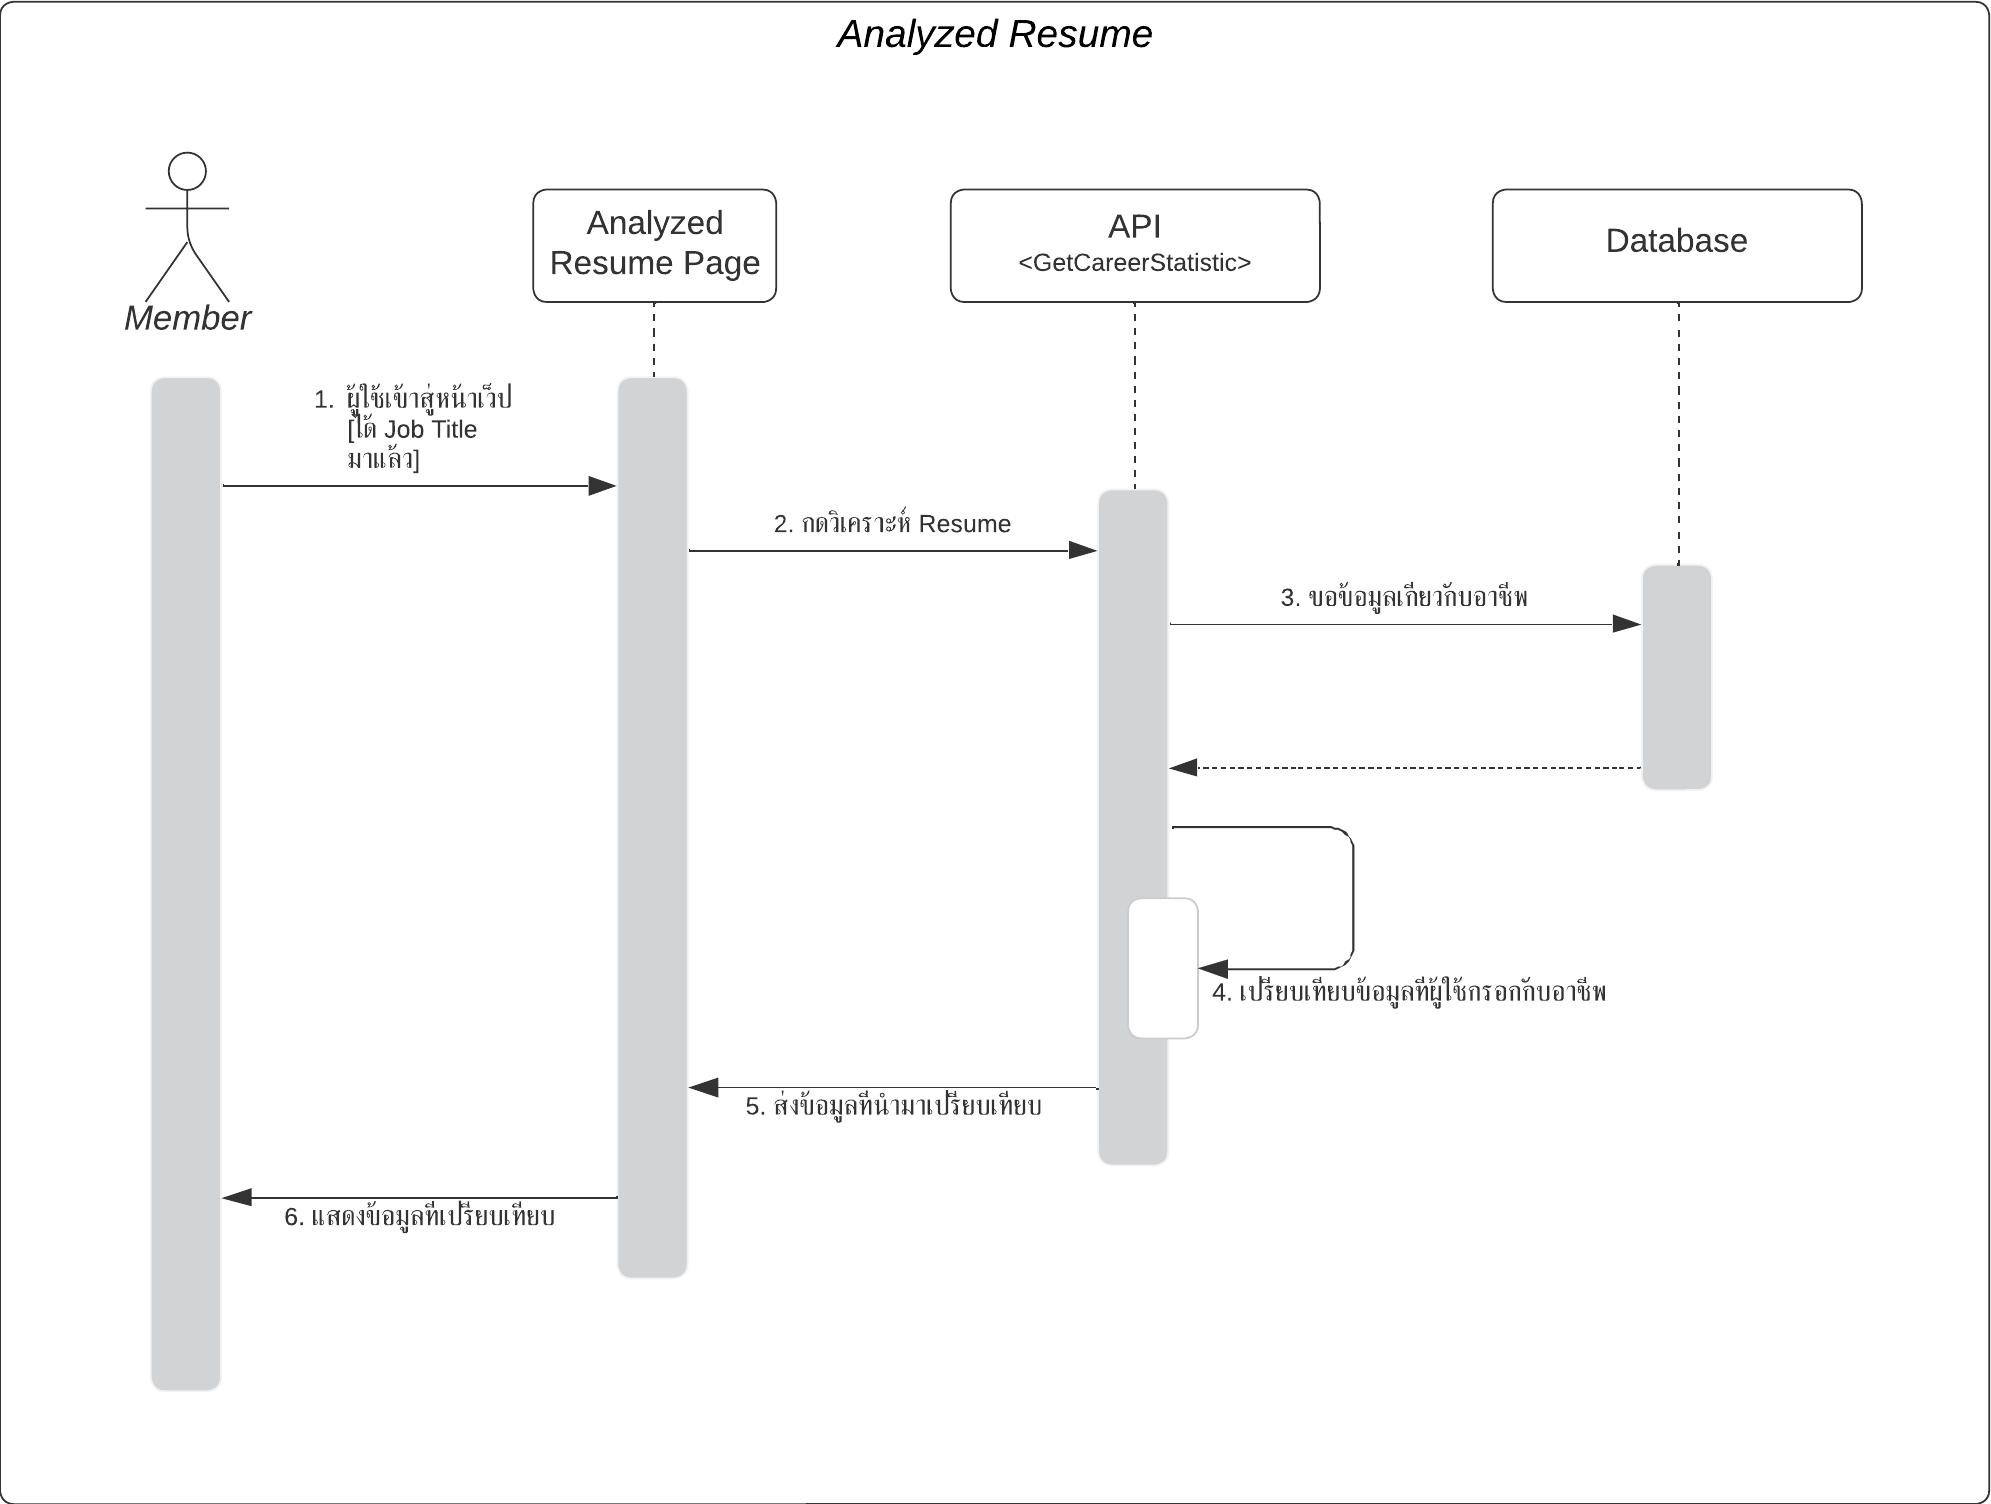
\includegraphics[width=8cm]{./figure/sequence-diagram/figure_sequence_analyze_resume.png}}
    \caption{Analyze Resume Sequence Diagram}\label{fig:anaResumeSeqDiagram}
\end{figure}
\textbf{สถานการณ์: }ผู้ใช้เข้าดูข้อมูลเชิงลึกจากการวิเคราะห์เรซูเม
\begin{enumerate}
    \item ผู้ใช้เข้าสู่หน้าวิเคราะห์ข้อมูลเชิงลึกจากช่องใดทางหนึ่ง เช่น ผ่านการ redirect จากหน้าวิเคราะห์เรซูเม หรือเข้าสู่หน้าข้อมูลเชิงลึกโดยตรง (ต้องมีข้อมูลมาก่อน)
    \item user interface ส่งคำขอสู่ระบบบริการหลัก และดึงข้อมูลจากฐานข้อมูล
    \item บริการหลักคำนวณข้อมูลและส่งกลับสู่ผู้ใช้
    \item แสดงผลแก่ผู้ใช้
\end{enumerate}

\subsection{View Forum}
\begin{figure}[H]\centering
    \setlength{\fboxrule}{0.2mm} % can define this in the preamble
    \fbox{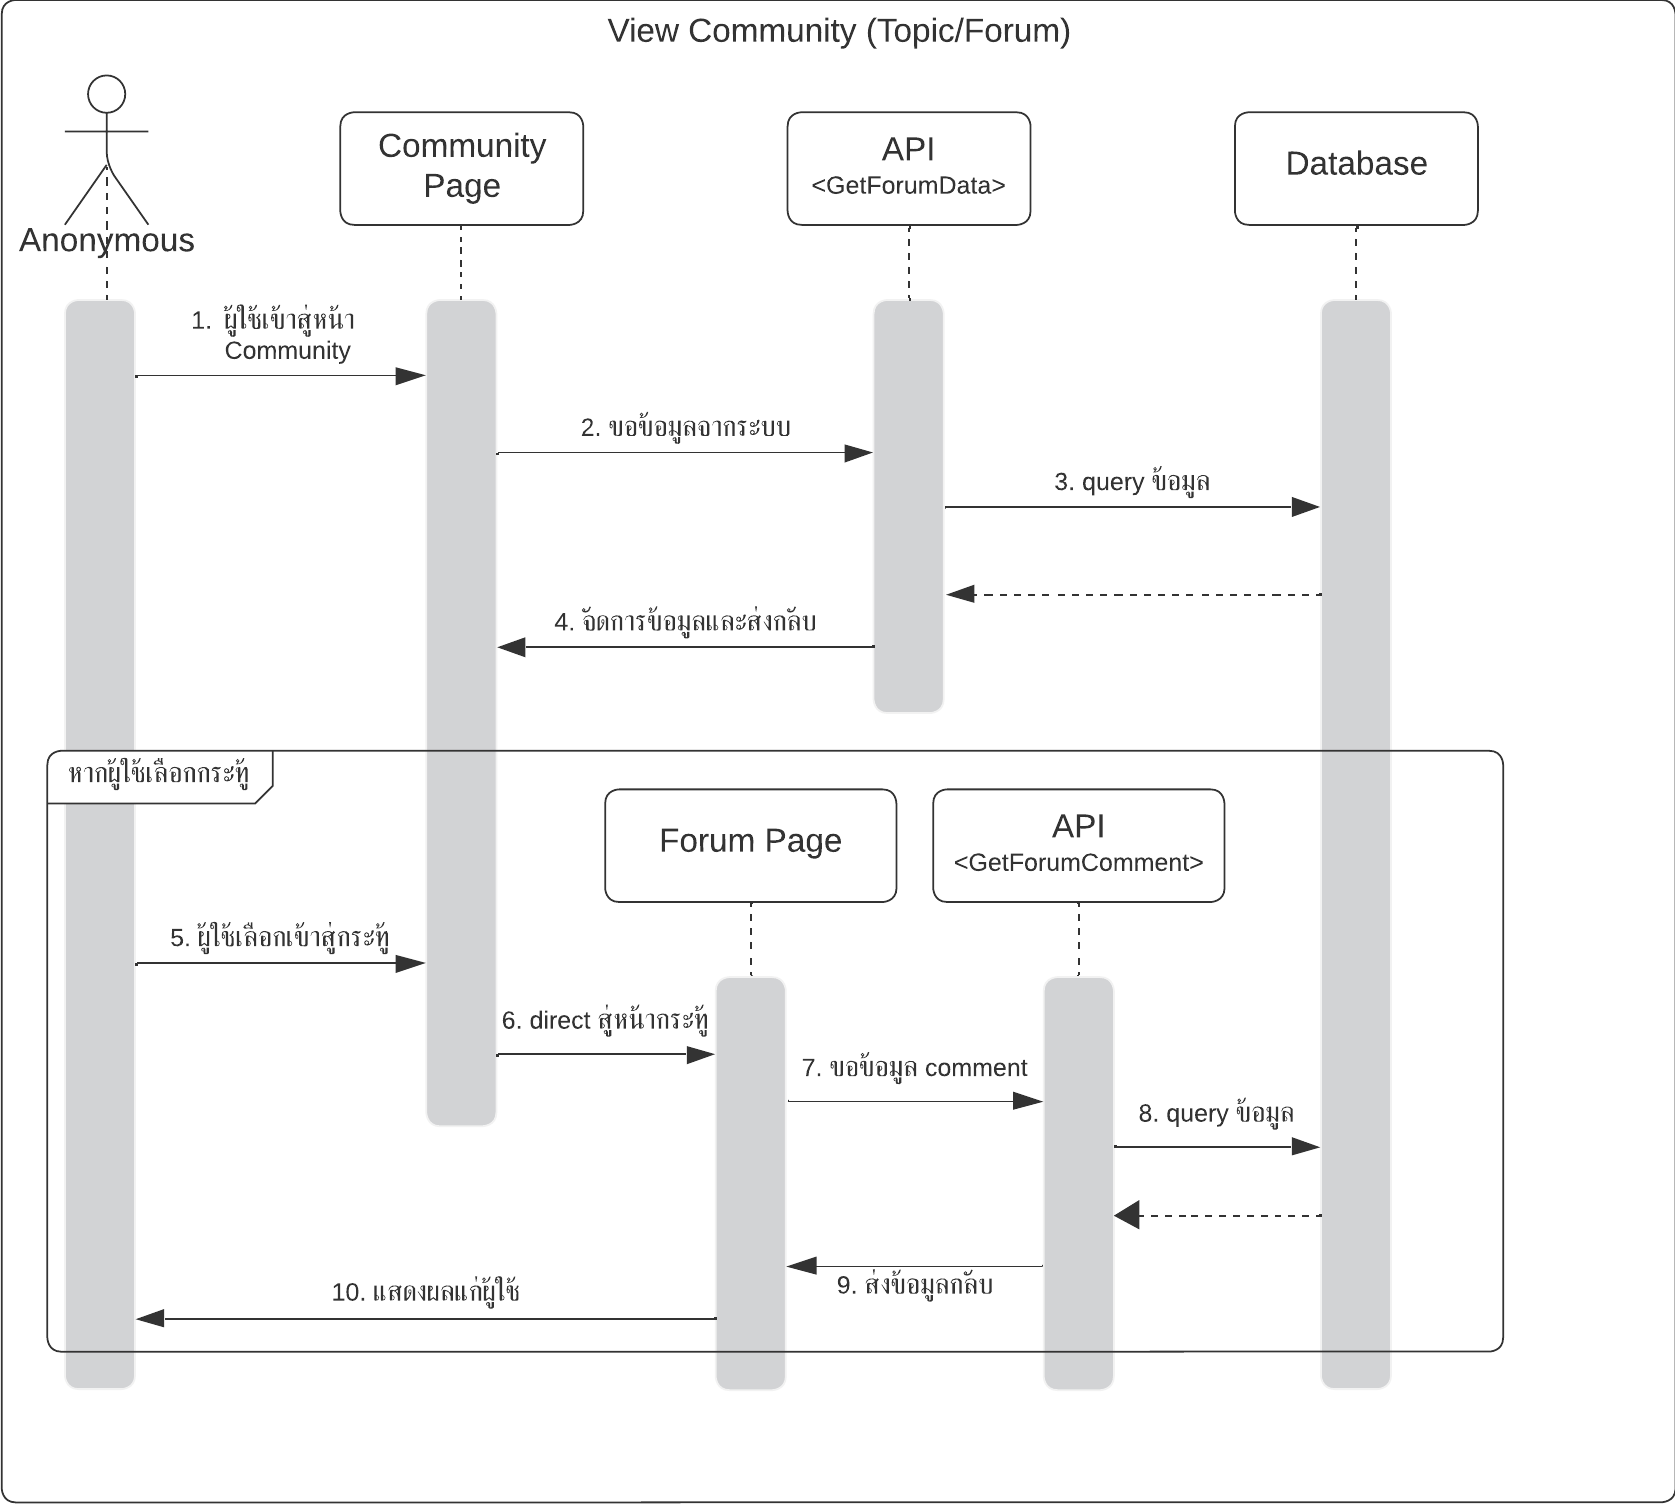
\includegraphics[width=8cm]{./figure/sequence-diagram/figure_sequence_view_forum.png}}
    \caption{View Forum Sequence Diagram}\label{fig:viewForumSeqDiagram}
\end{figure}
\textbf{สถานการณ์: }ผู้ใช้เข้าดูหน้าชุมชน
\begin{enumerate}
    \item ผู้ใช้เข้ากดเข้าสู่หน้าชุมชน
    \item user interface ส่งคำขอสู่ระบบบริการหลักและดึงข้อมูลจากฐานข้อมูล
    \item บริการหลักส่งข้อมูลกลับสู่ผู้ใช้และแสดงผล
\end{enumerate}

\subsection{Reply Forum}
\begin{figure}[H]\centering
    \setlength{\fboxrule}{0.2mm} % can define this in the preamble
    \fbox{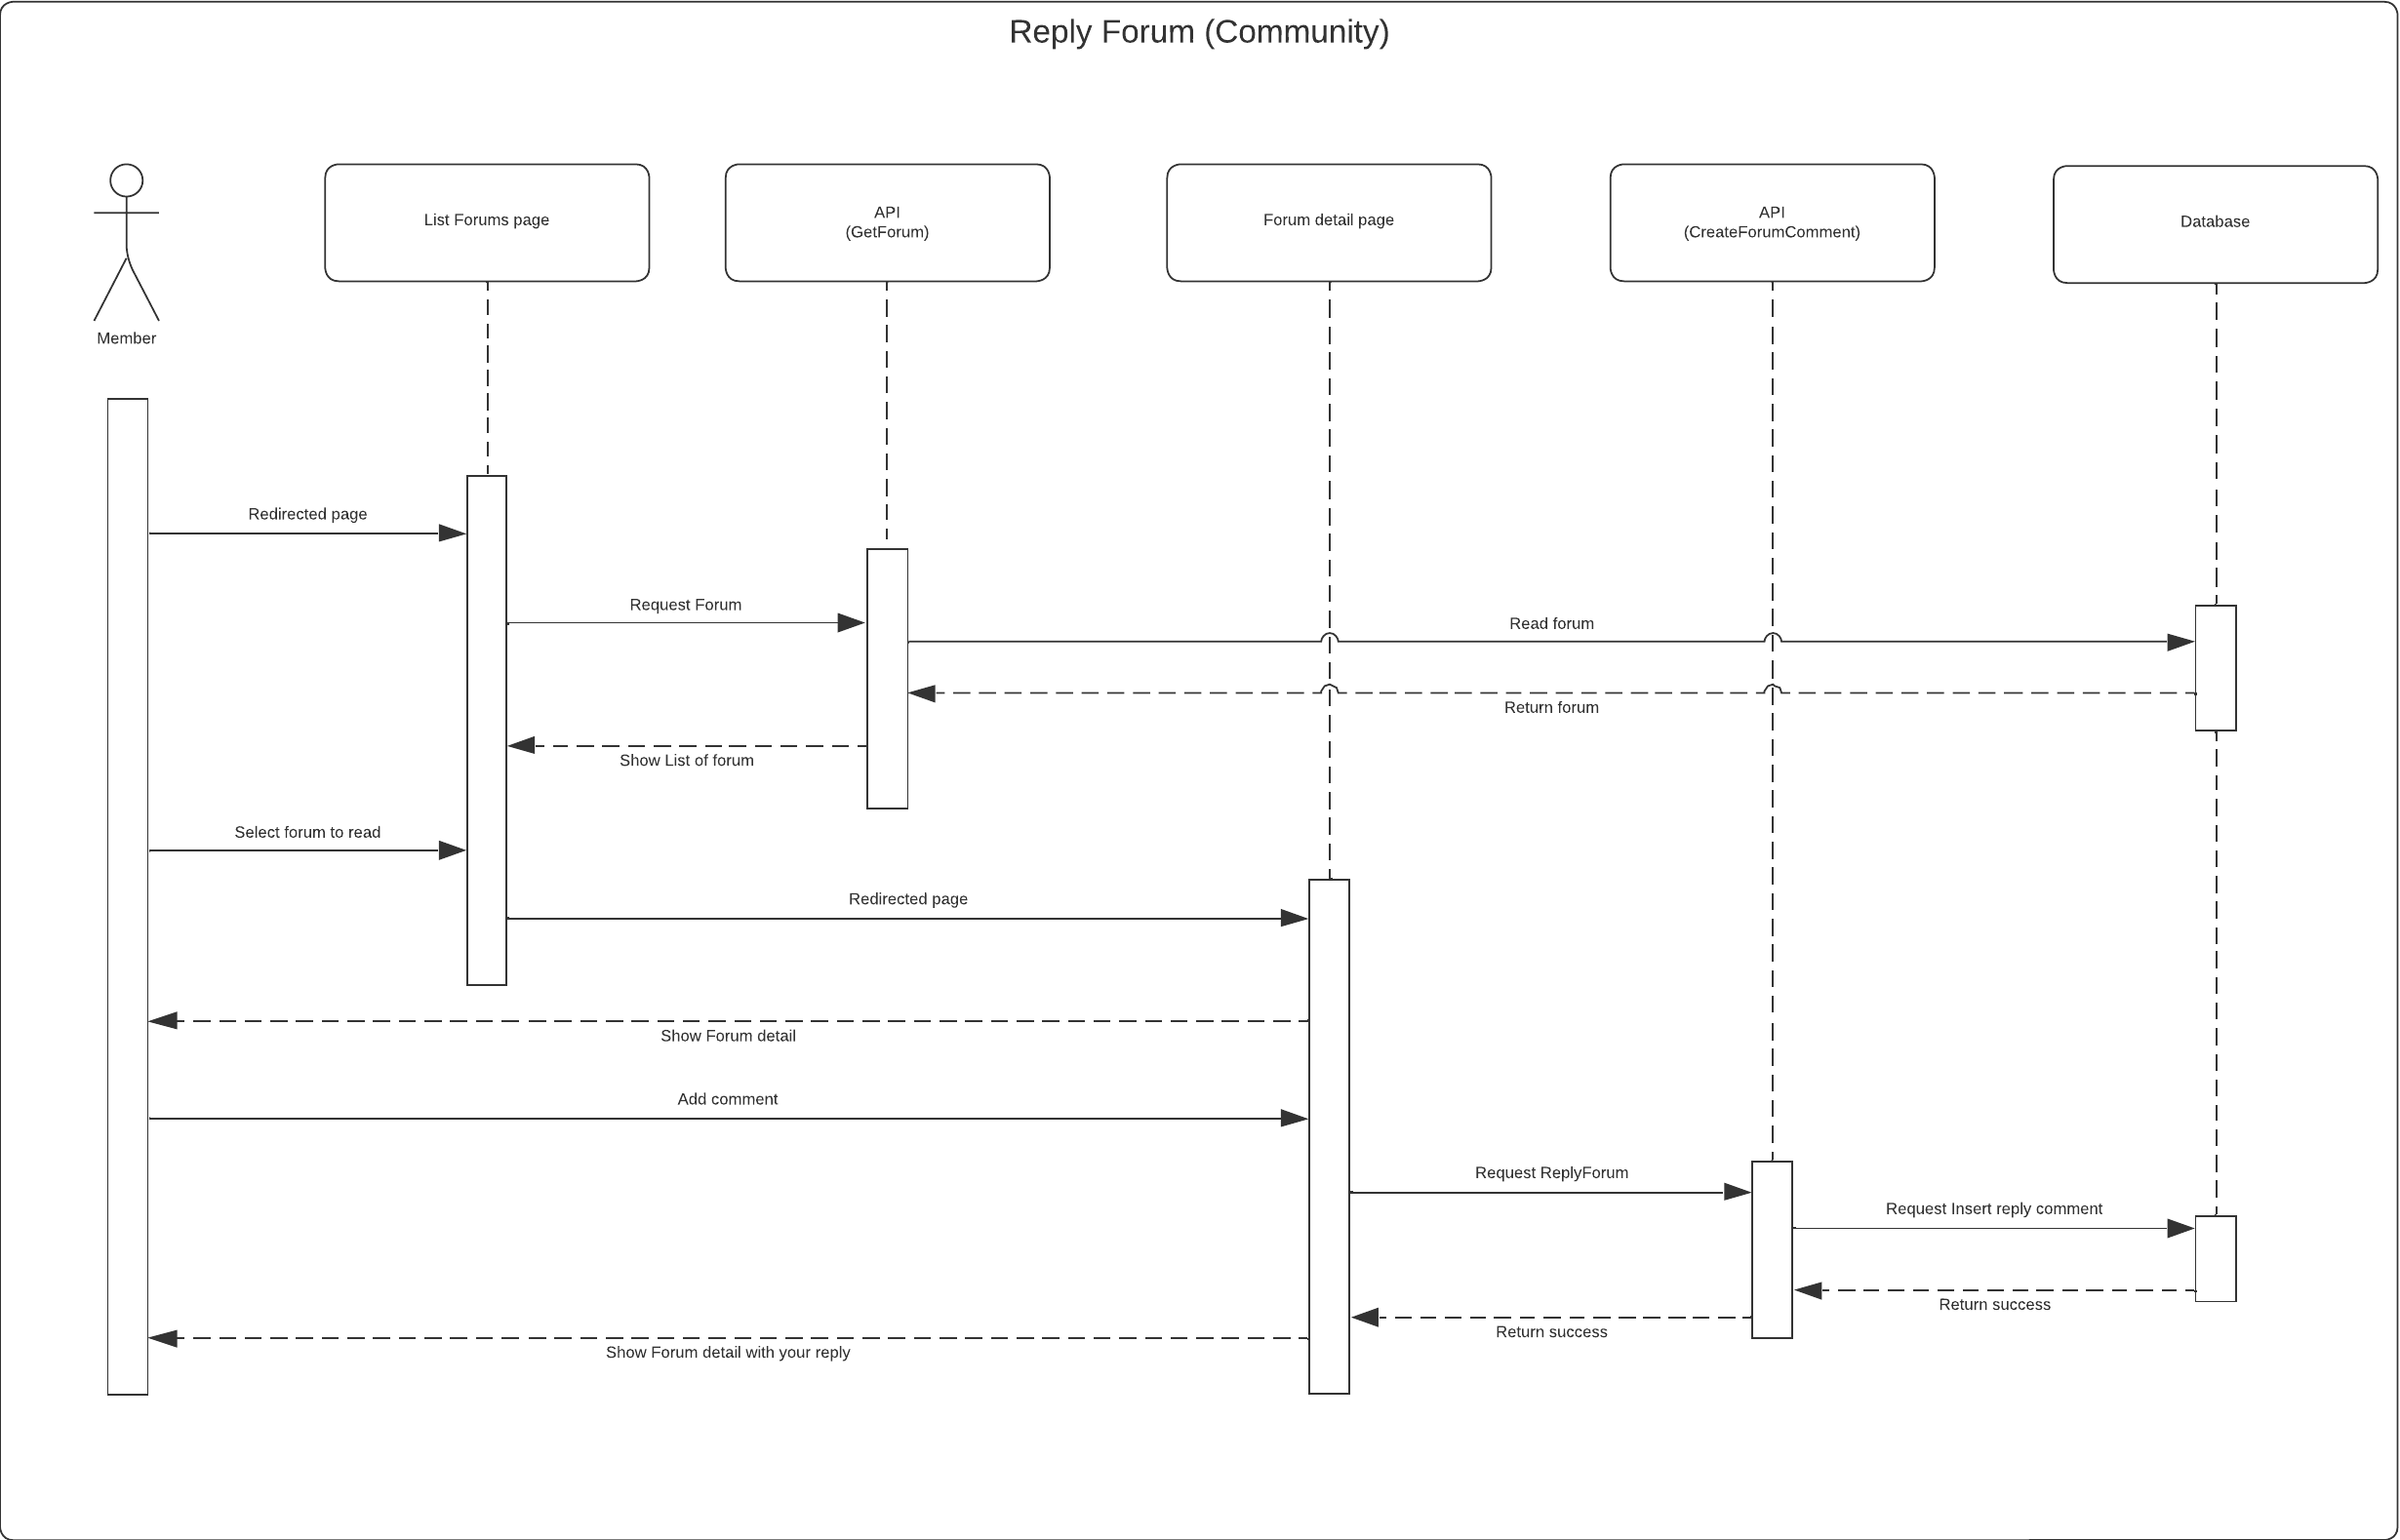
\includegraphics[width=8cm]{./figure/sequence-diagram/figure_sequence_reply_forum.png}}
    \caption{Reply Forum Sequence Diagram}\label{fig:ReplyForumSeqDiagram}
\end{figure}
\textbf{สถานการณ์: }ผู้ใช้ตอบกลับข้อความในกระทู้ชุมชน
\begin{enumerate}
    \item ผู้ใช้กดเข้าหน้าเลือกกระทู้จากชุมชน
    \item user interface ส่งคำขอสู่บริการหลัก เพื่อดึงข้อมูลจากฐานข้อมูล
    \item ส่งรายการกระทู้กลับสู่ผู้ใช้
    \item ผู้ใช้เลือกกระทู้และเข้าสู่หน้ากระทู้
    \item ผู้ใช้กดพิมพ์ข้อความและกดตอบกลับกระทู้
    \item user interface ทำการส่งข้อมูลสู่บริการหลักเพื่อบันทุกข้อความใหม่นี้สู่ฐานข้อมูล
    \item ส่งสถานะสำเร็จแก่ผู้ใช้และแสดงผล
\end{enumerate}

\subsection{Create Forum}
\begin{figure}[H]\centering
    \setlength{\fboxrule}{0.2mm} % can define this in the preamble
    \fbox{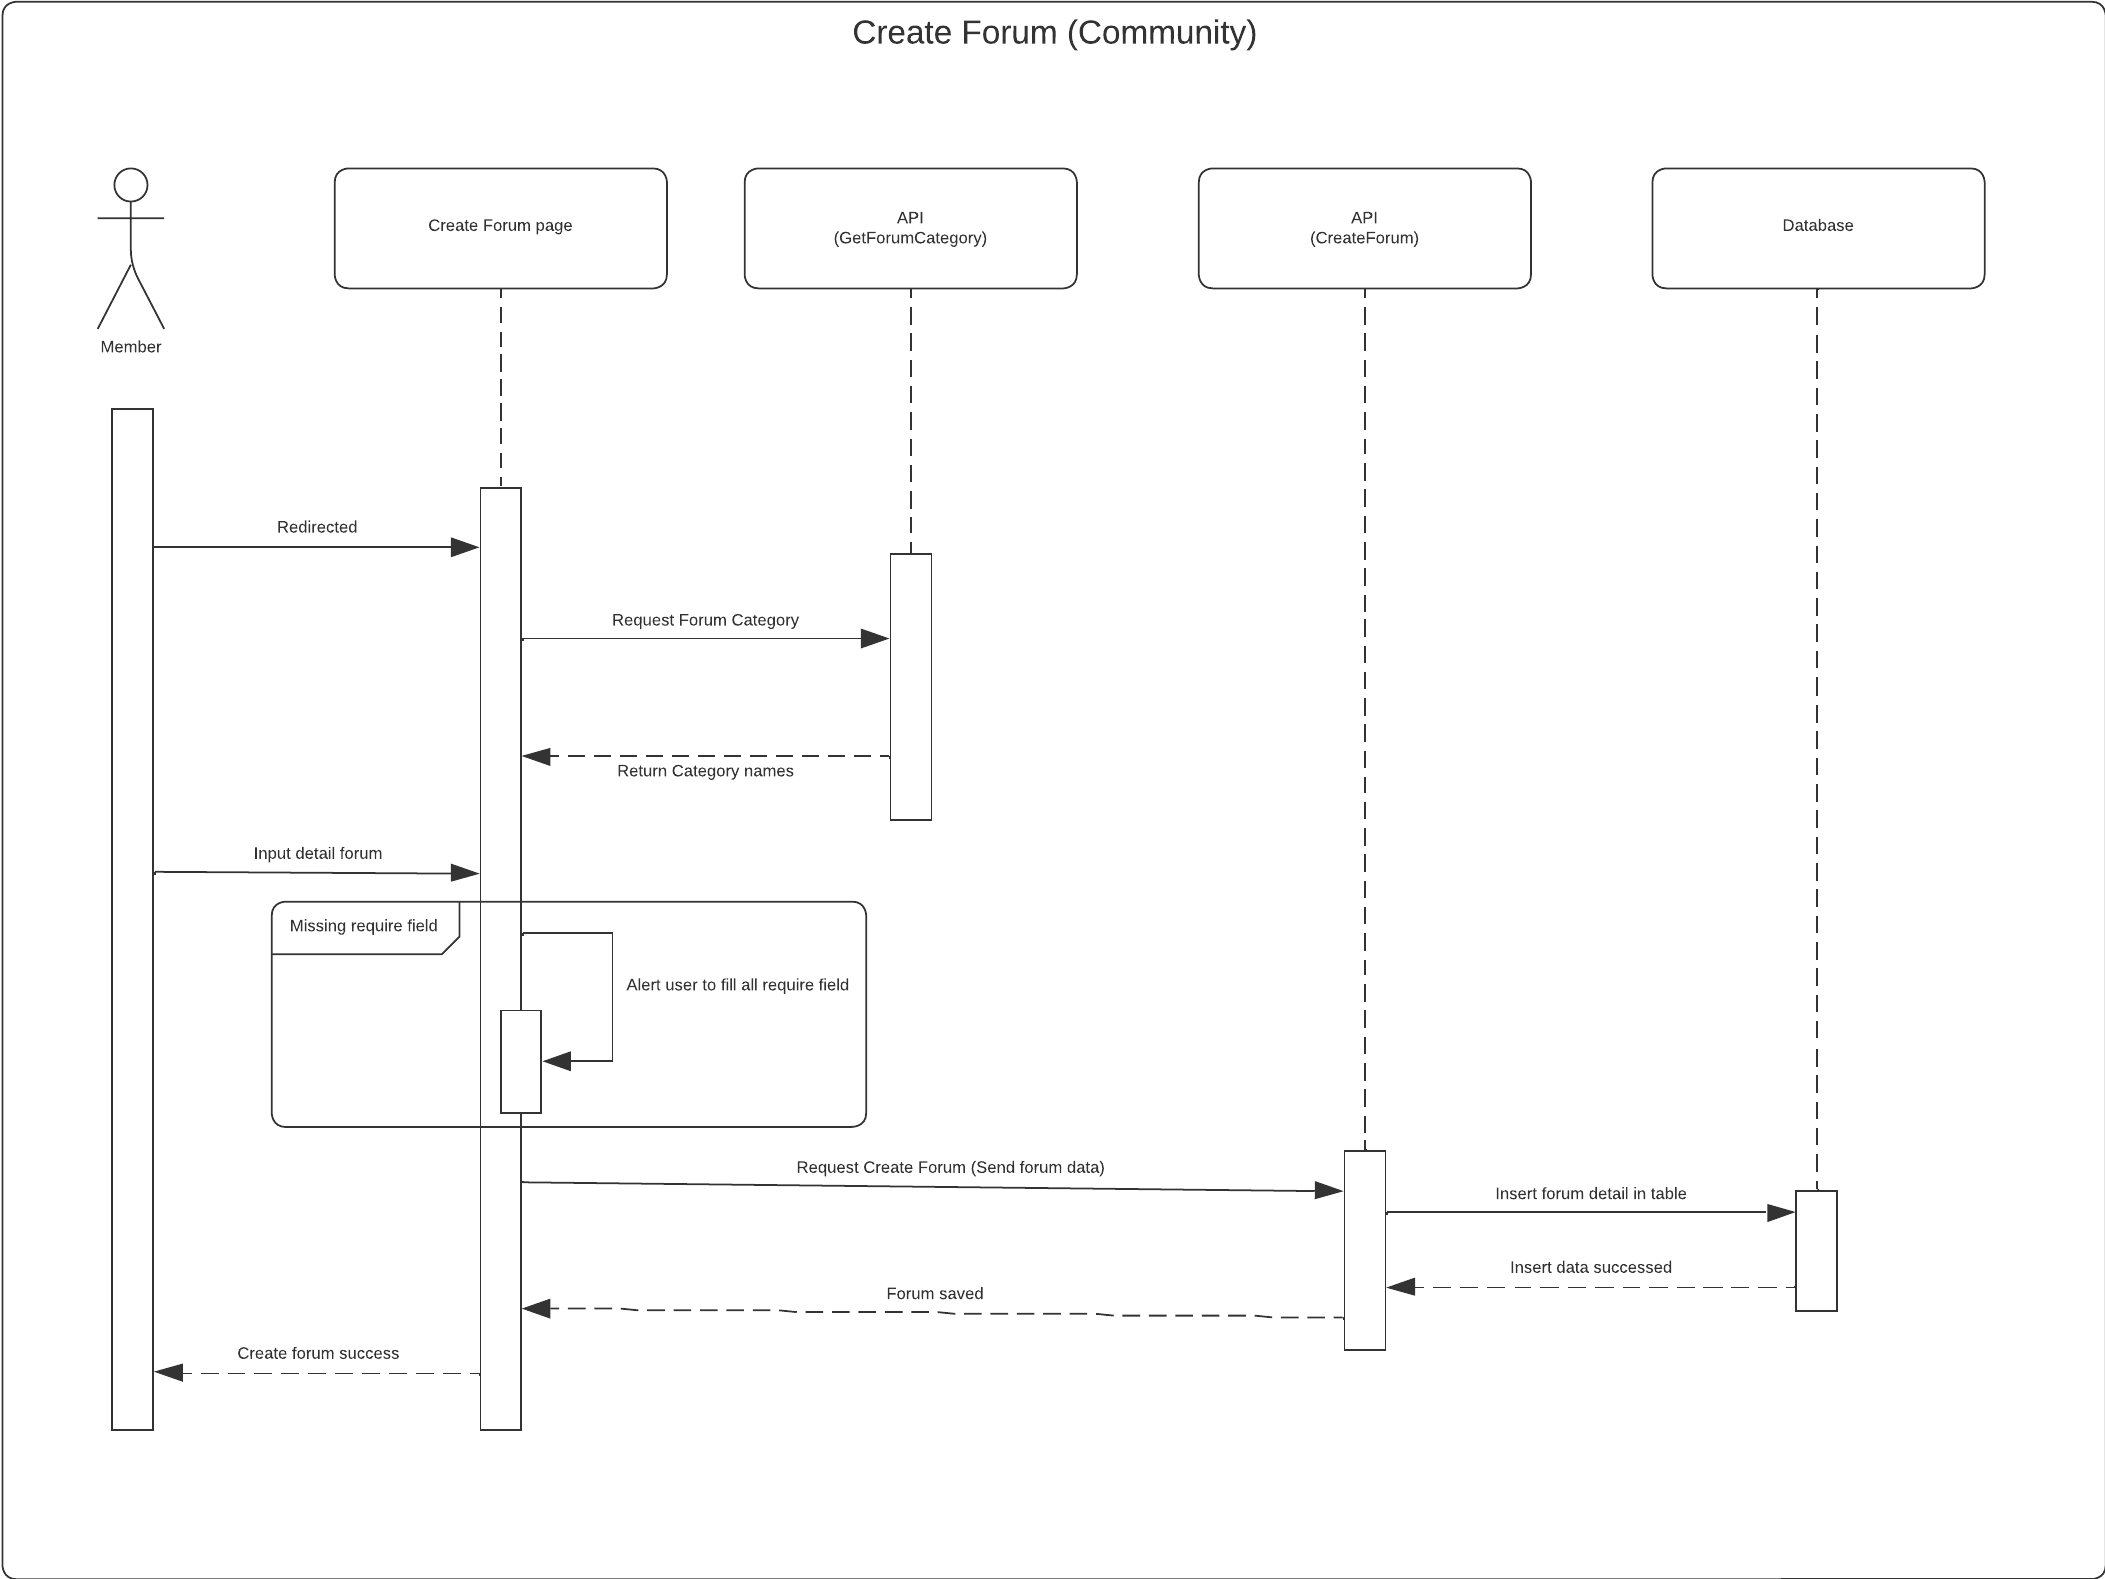
\includegraphics[width=8cm]{./figure/sequence-diagram/figure_sequence_create_forum.png}}
    \caption{Create Forum Sequence Diagram}\label{fig:createForumSeqDiagram}
\end{figure}
\textbf{สถานการณ์: }ผู้ใช้สร้างกระทู้ใหม่
\begin{enumerate}
    \item ผู้ใช้กดสร้างกระทู้ใหม่
    \item user interface ส่งคำขอจากบริการหลักเพื่อดึงข้อมูลประเภทกระทู้ที่อาจมีได้ และส่งกลับสู่ผู้ใช้
    \item ผู้ใช้เลือกประเภทของกระทู้และกรอกข้อมูลกระทู้ทั้งหมด
    \item user interface ตรวจสอบข้อมูลที่ผู้ใช้กรอก หากผิดพลาดจะแจ้งเตือนแก่ผู้ใช้ หากไม่มีปัญหาจะส่งคำขอสู่บริการหลัก
    \item บริการหลักบันทึกข้อมูลกระทู้ลงสู่ฐานข้อมูล และส่งสถานะกลับสู่ผู้ใช้ พร้อมแสดงผล
\end{enumerate}

\subsection{See Career Node Tree}
\begin{figure}[H]\centering
    \setlength{\fboxrule}{0.2mm} % can define this in the preamble
    \fbox{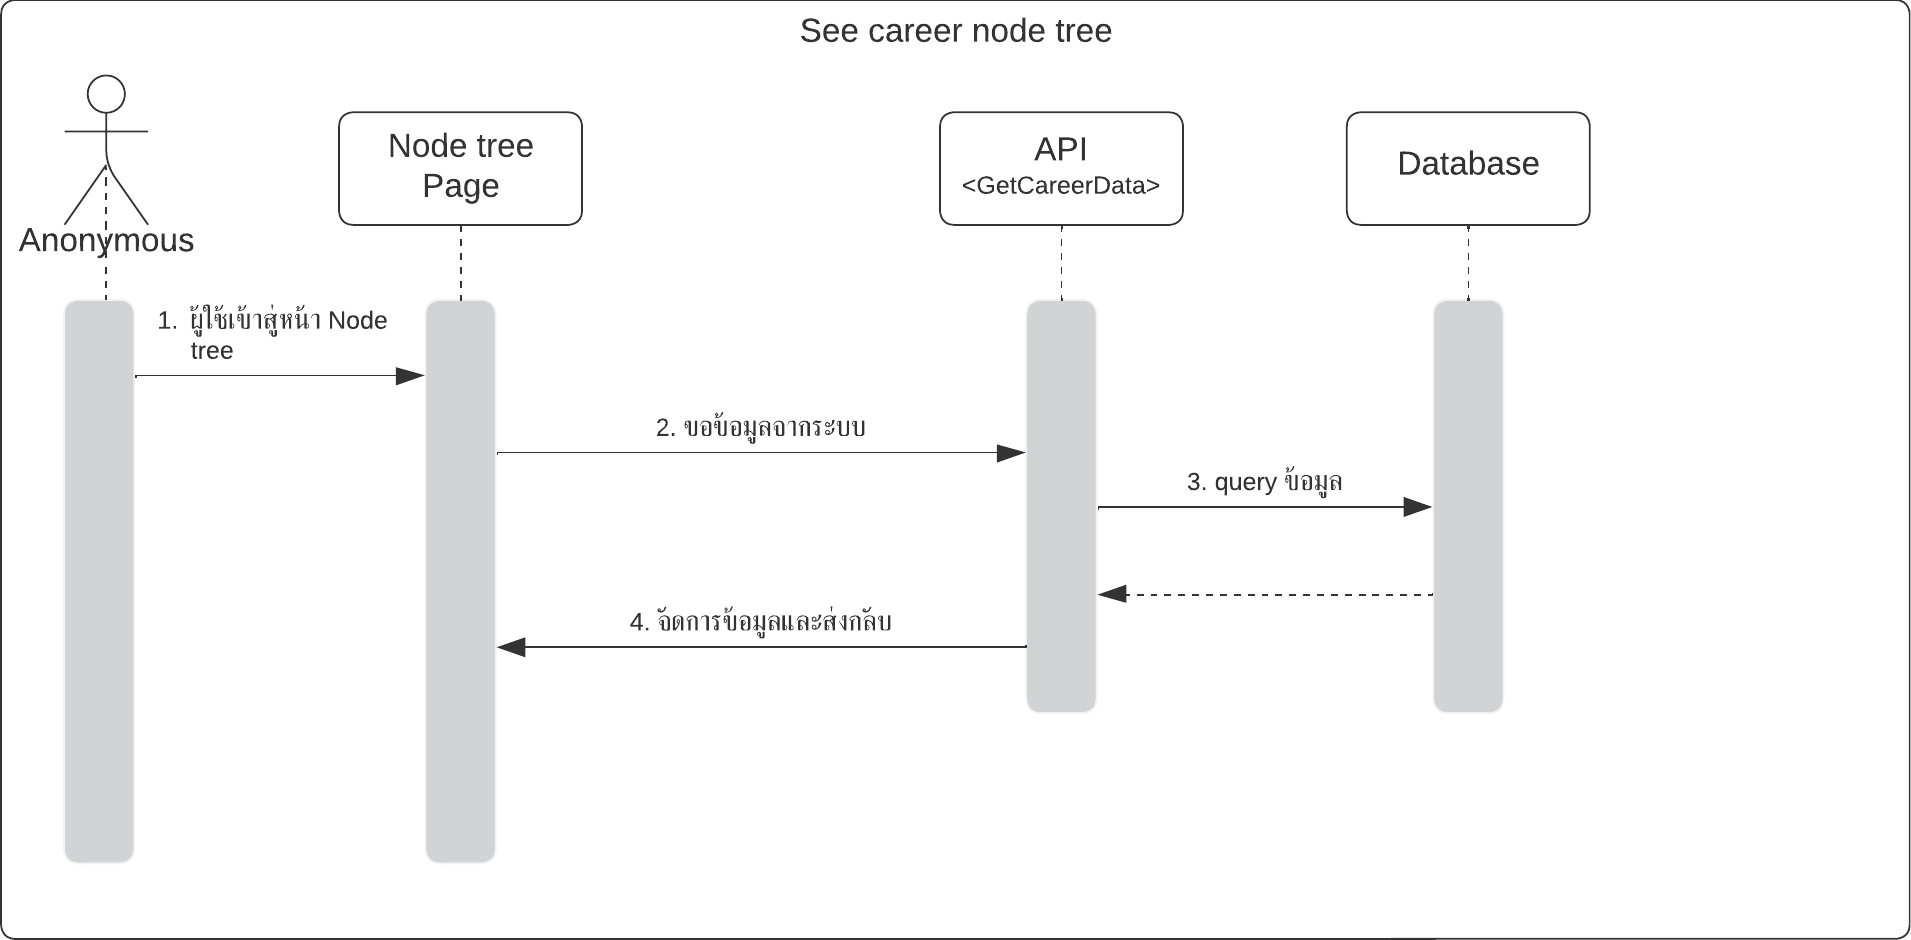
\includegraphics[width=8cm]{./figure/sequence-diagram/figure_sequence_see_node.png}}
    \caption{See Career Node Tree Sequence Diagram}\label{fig:nodeTreeSeqDiagram}
\end{figure}
\textbf{สถานการณ์: }ผู้ใช้เข้าดูหน้าสายใยอาชีพ
\begin{enumerate}
    \item ผู้ใช้เข้าสู่หน้าสายใยอาชีพ
    \item user interface ขอข้อมูลจากบริการหลักและดึงข้อมูลจากฐานข้อมูล
    \item บริการหลักส่งข้อมูลกลับสู่ผู้ใช้และแสดงผล
\end{enumerate}

\section{Database}
ระบบฐานข้อมูลของเราจะใช้เป็นรูปแบบ NoSQL ประเภท document ผ่านบริการของ MongoDB โดยมีรายละเอียดในแต่ละตาราง ดังนี้
\begin{figure}[H]\centering
  \setlength{\fboxrule}{0.2mm} % can define this in the preamble
  \setlength{\fboxsep}{0.5cm}
  \fbox{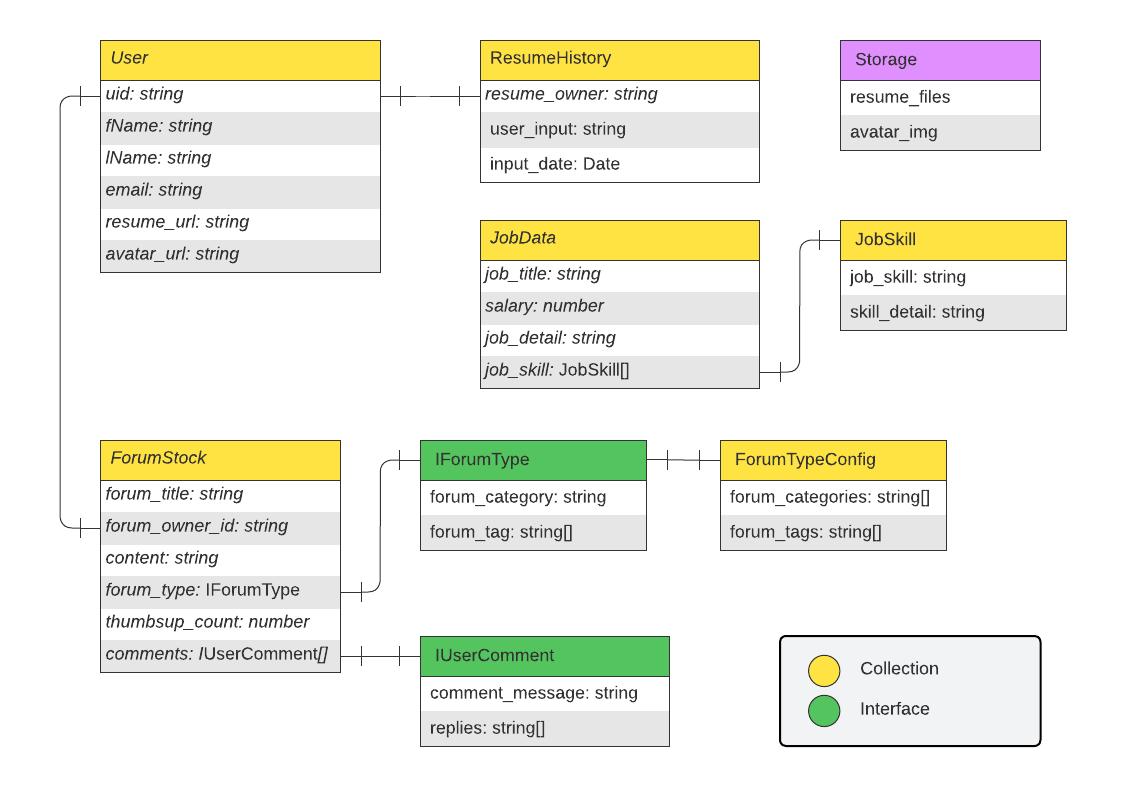
\includegraphics[width=8cm]{./figure/figure_database.png}}
  \caption{Database Structure}\label{fig:database}
\end{figure}

\begin{table}[H]
  \begin{tabular*}{\textwidth}{l|l|p{0.6\textwidth}}
  \hline
  \multicolumn{3}{c}{User}                                                                                                      \\ \hline
  Field Name  & Field Type & Description                                                                                        \\ \hline
  uid         & string     & รหัสประจำตัวของผู้ใช้ ที่ทางระบบจะเป็นผู้กำหนดให้ เพื่อใช้แยกผู้ใช้แต่ละท่านอย่างชัดเจน            \\
  fName       & string     & ชื่อต้นของผู้ใช้                                                                                   \\
  lName       & string     & นามสกุลของผู้ใช้                                                                                   \\
  email       & string     & อีเมลของผู้ใช้                                                                                     \\
  resume\_url & string     & url สำหรับเข้าถึงไฟล์ resume ที่ผู้ใช้อัพโหลดสู่ระบบของเรา โดยระบบจะบบจะเป็นผู้จัดการข้อมูลส่วนนี้ \\
  avatar\_url & string     & url สำหรับเข้าถึงรูปโปรไฟล์ผู้ใช้ โดยระบบจะบบจะเป็นผู้จัดการข้อมูลส่วนนี้                          \\ \hline
  \end{tabular*}
\end{table}

\begin{table}[H]
  \begin{tabular*}{\textwidth}{l|l|p{0.6\textwidth}}
  \hline
  \multicolumn{3}{c}{ResumeHistory}                                                                   \\\hline
  Field Name    & Field Type & Description                                                            \\\hline
  resume\_owner & string     & รหัสประจำตัวของผู้ใช้ รูปแบบเดียวกับ uid ใช้สำหรับการระบุเจ้าของข้อมูล \\
  user\_input   & string     & ค่ารับเข้าจากผู้ใช้                                                    \\
  input\_date   & Date       & วันที่ผู้ใช้กรอกข้อมูล \\ \hline
  \end{tabular*}
\end{table}

\begin{table}[H]
  \begin{tabular*}{\textwidth}{l|l|p{0.6\textwidth}}
  \hline
    \multicolumn{3}{c}{ForumStock}  \\ \hline                                                                                                     
    Field Name      & Field Type         & Description                                                                             \\\hline
    forum\_title    & string             & ชื่อหัวข้อกระทู้                                                                                \\
    forum\_owner    & string             & uid ของผู้ใช้ที่เป็นเจ้าของกระทู้ ใช้สำหรับระบุตัวตน                                            \\
    content         & string             & เนื้อหาหลักของกระทู้                                                                            \\
    forum\_type     & IForumType         & ประเภทของกระทู้ มีรูปแบบข้อมูลเป็น object ของประเภทกระทู้และ ชุดข้อมูลของ tag ที่เกี่ยวข้อง     \\
    thumbups\_count & number             & จำนวนของการกดถูกใจกระทู้                                                                        \\
    comments        & IUserComment{[}{]} & ความเห็นภายในกระทู้ มีรูปแบบข้อมูลเป็น object ของความเห็นหลักและข้อความตอบกลับภายในความเห็นนั้น \\ \hline
  \end{tabular*}
\end{table}

\begin{table}[H]
  \begin{tabular*}{\textwidth}{l|l|p{0.6\textwidth}}
  \hline
    \multicolumn{3}{c}{ForumTypeConfig}                                           \\\hline  
    Field Name        & Field Type   & Description                                \\\hline  
    forum\_categories & string{[}{]} & ประเภททั้งหมดของกระทู้ที่สามารถมีได้ในระบบ \\
    forum\_tags       & string{[}{]} & tag ของกระทู้ทั้งหมดที่สามารถมีได้ในระบบ \\ \hline  
  \end{tabular*}
\end{table}

\begin{table}[H]
  \begin{tabular*}{\textwidth}{l|l|p{0.6\textwidth}}
  \hline
    \multicolumn{3}{c}{JobData}                                                                      \\\hline
    Field Name  & Field Type     & Description                                                       \\\hline
    job\_title  & string         & ชื่อของอาชีพ                                                      \\
    salary      & number         & ฐานเงินเดือนของอาชีพนั้น                                          \\
    job\_detail & string         & ข้อมูลเบื้องต้นของอาชีพนั้น                                       \\
    job\_skill  & JobSkill{[}{]} & ข้อมูลความสามารถของอาชีพนั้น มีรูปแบบและข้อมูลมาจากตาราง JobSkill \\ \hline
  \end{tabular*}
\end{table}

\begin{table}[H]
  \begin{tabular*}{\textwidth}{l|l|p{0.6\textwidth}}
  \hline
    \multicolumn{3}{c}{JobSkill}                              \\\hline
    Field Name    & Field Type & Description                  \\\hline
    job\_skill    & string     & ชื่อของความสามารถนั้นๆ       \\
    skill\_detail & string     & รายละเอียดของความสามารถนั้นๆ \\\hline
  \end{tabular*}
\end{table}

\section{Site Map}
\begin{figure}[H]\centering
    \setlength{\fboxrule}{0.2mm} % can define this in the preamble
    \setlength{\fboxsep}{0.5cm}
    \fbox{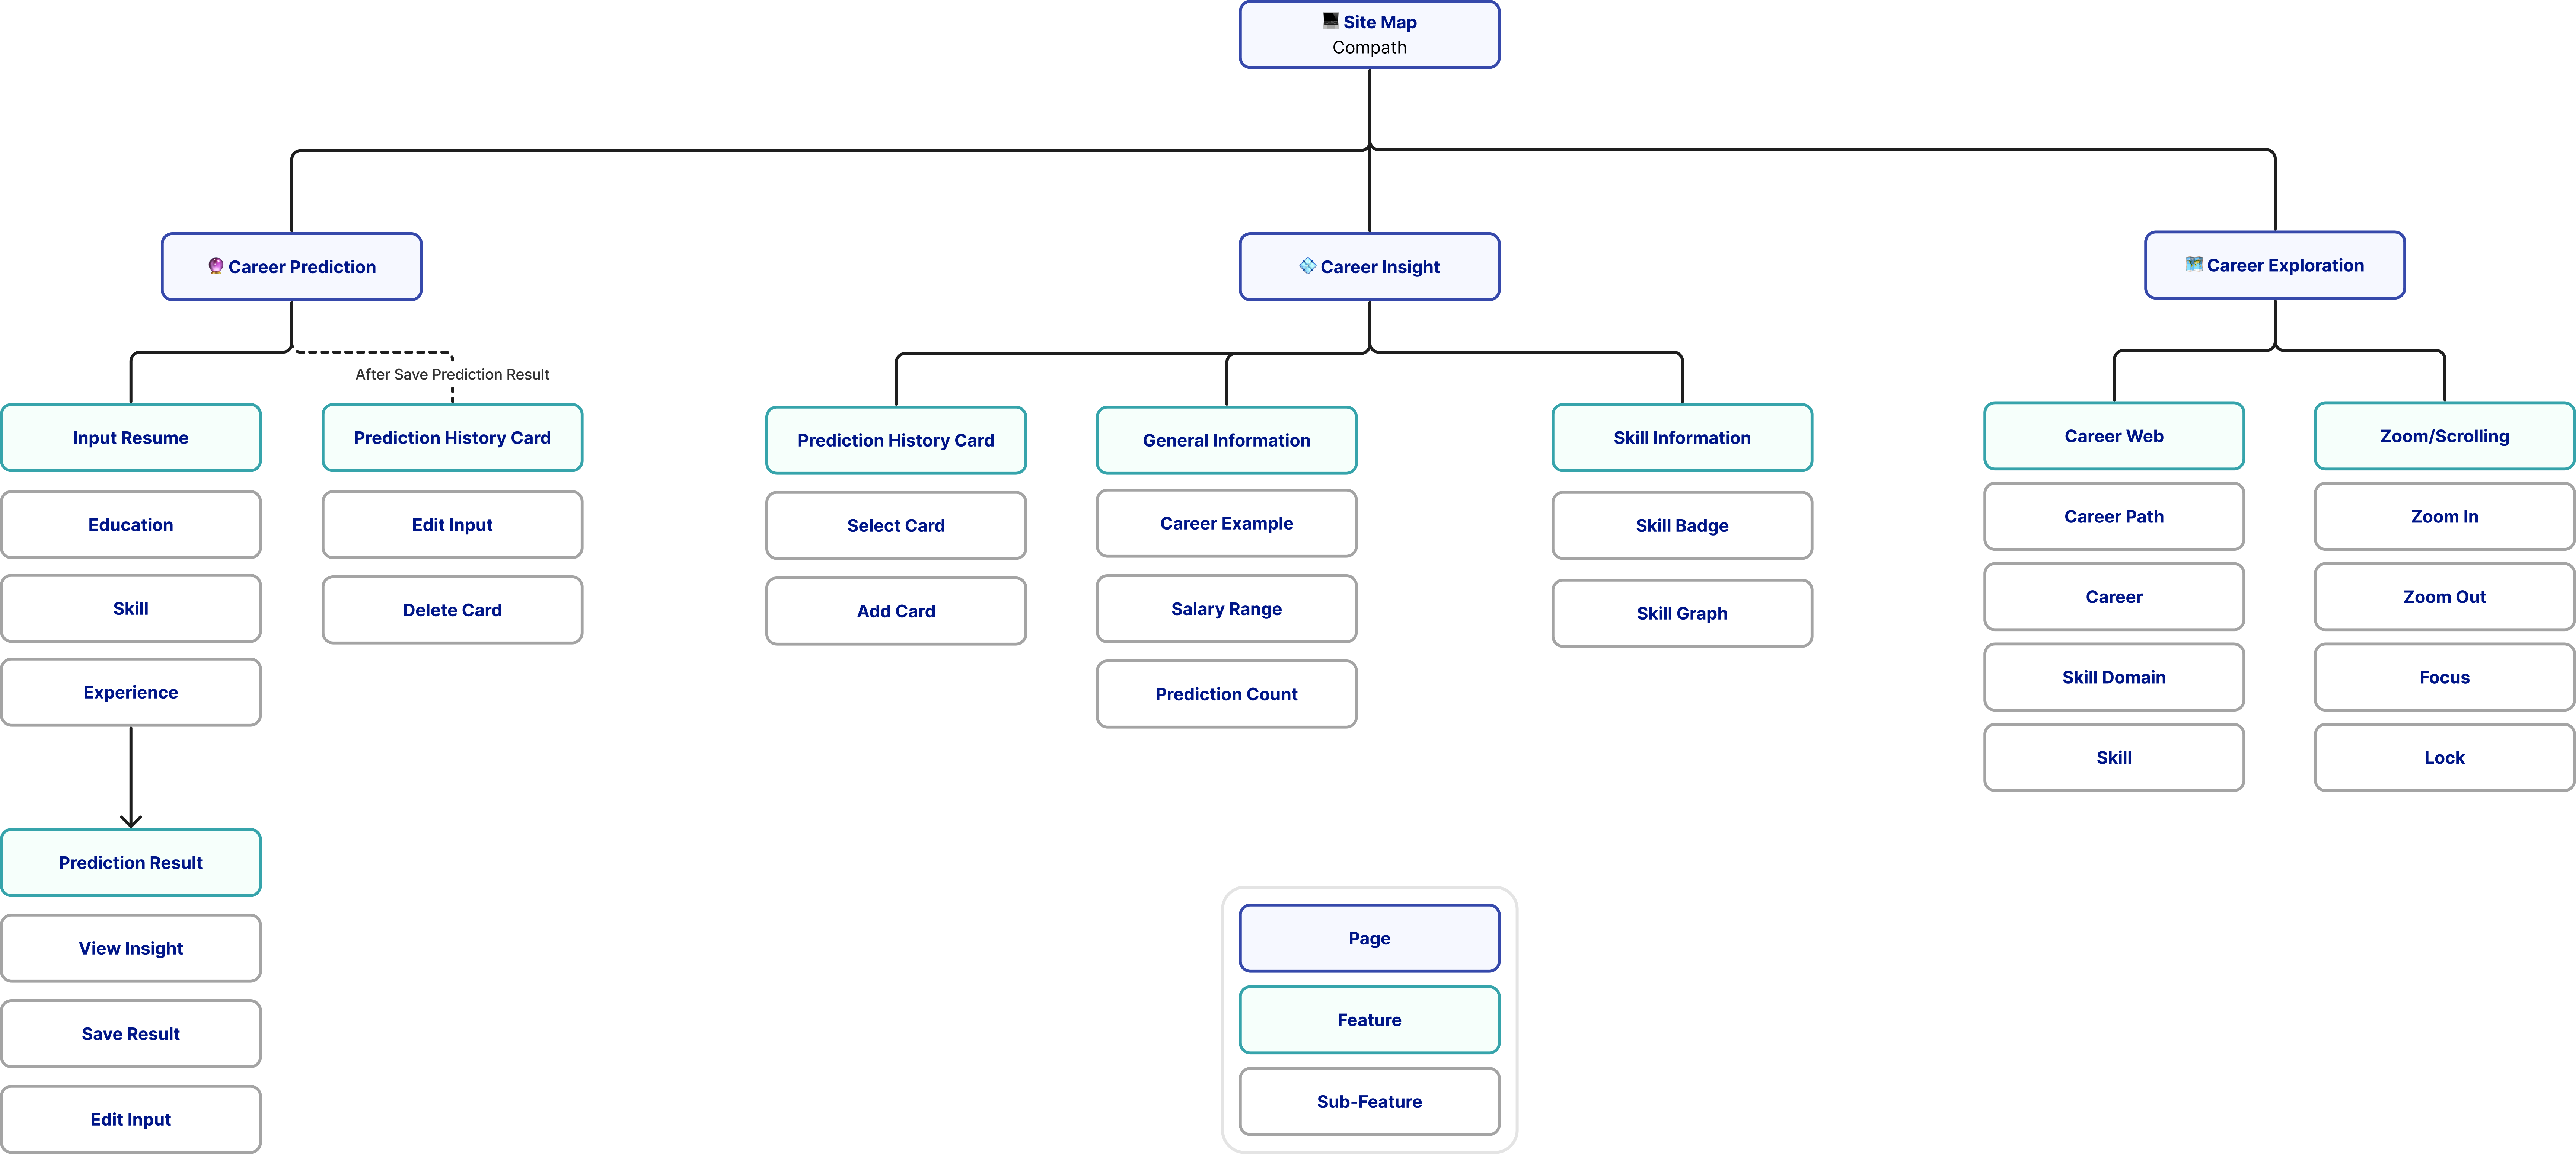
\includegraphics[width=10cm]{./figure/figure_siteMap.png}}
    \caption{SiteMap}\label{fig:siteMap}
\end{figure}

\section{Navigation Map}
\begin{figure}[H]\centering
    \setlength{\fboxrule}{0.2mm} % can define this in the preamble
    \setlength{\fboxsep}{0.5cm}
    \fbox{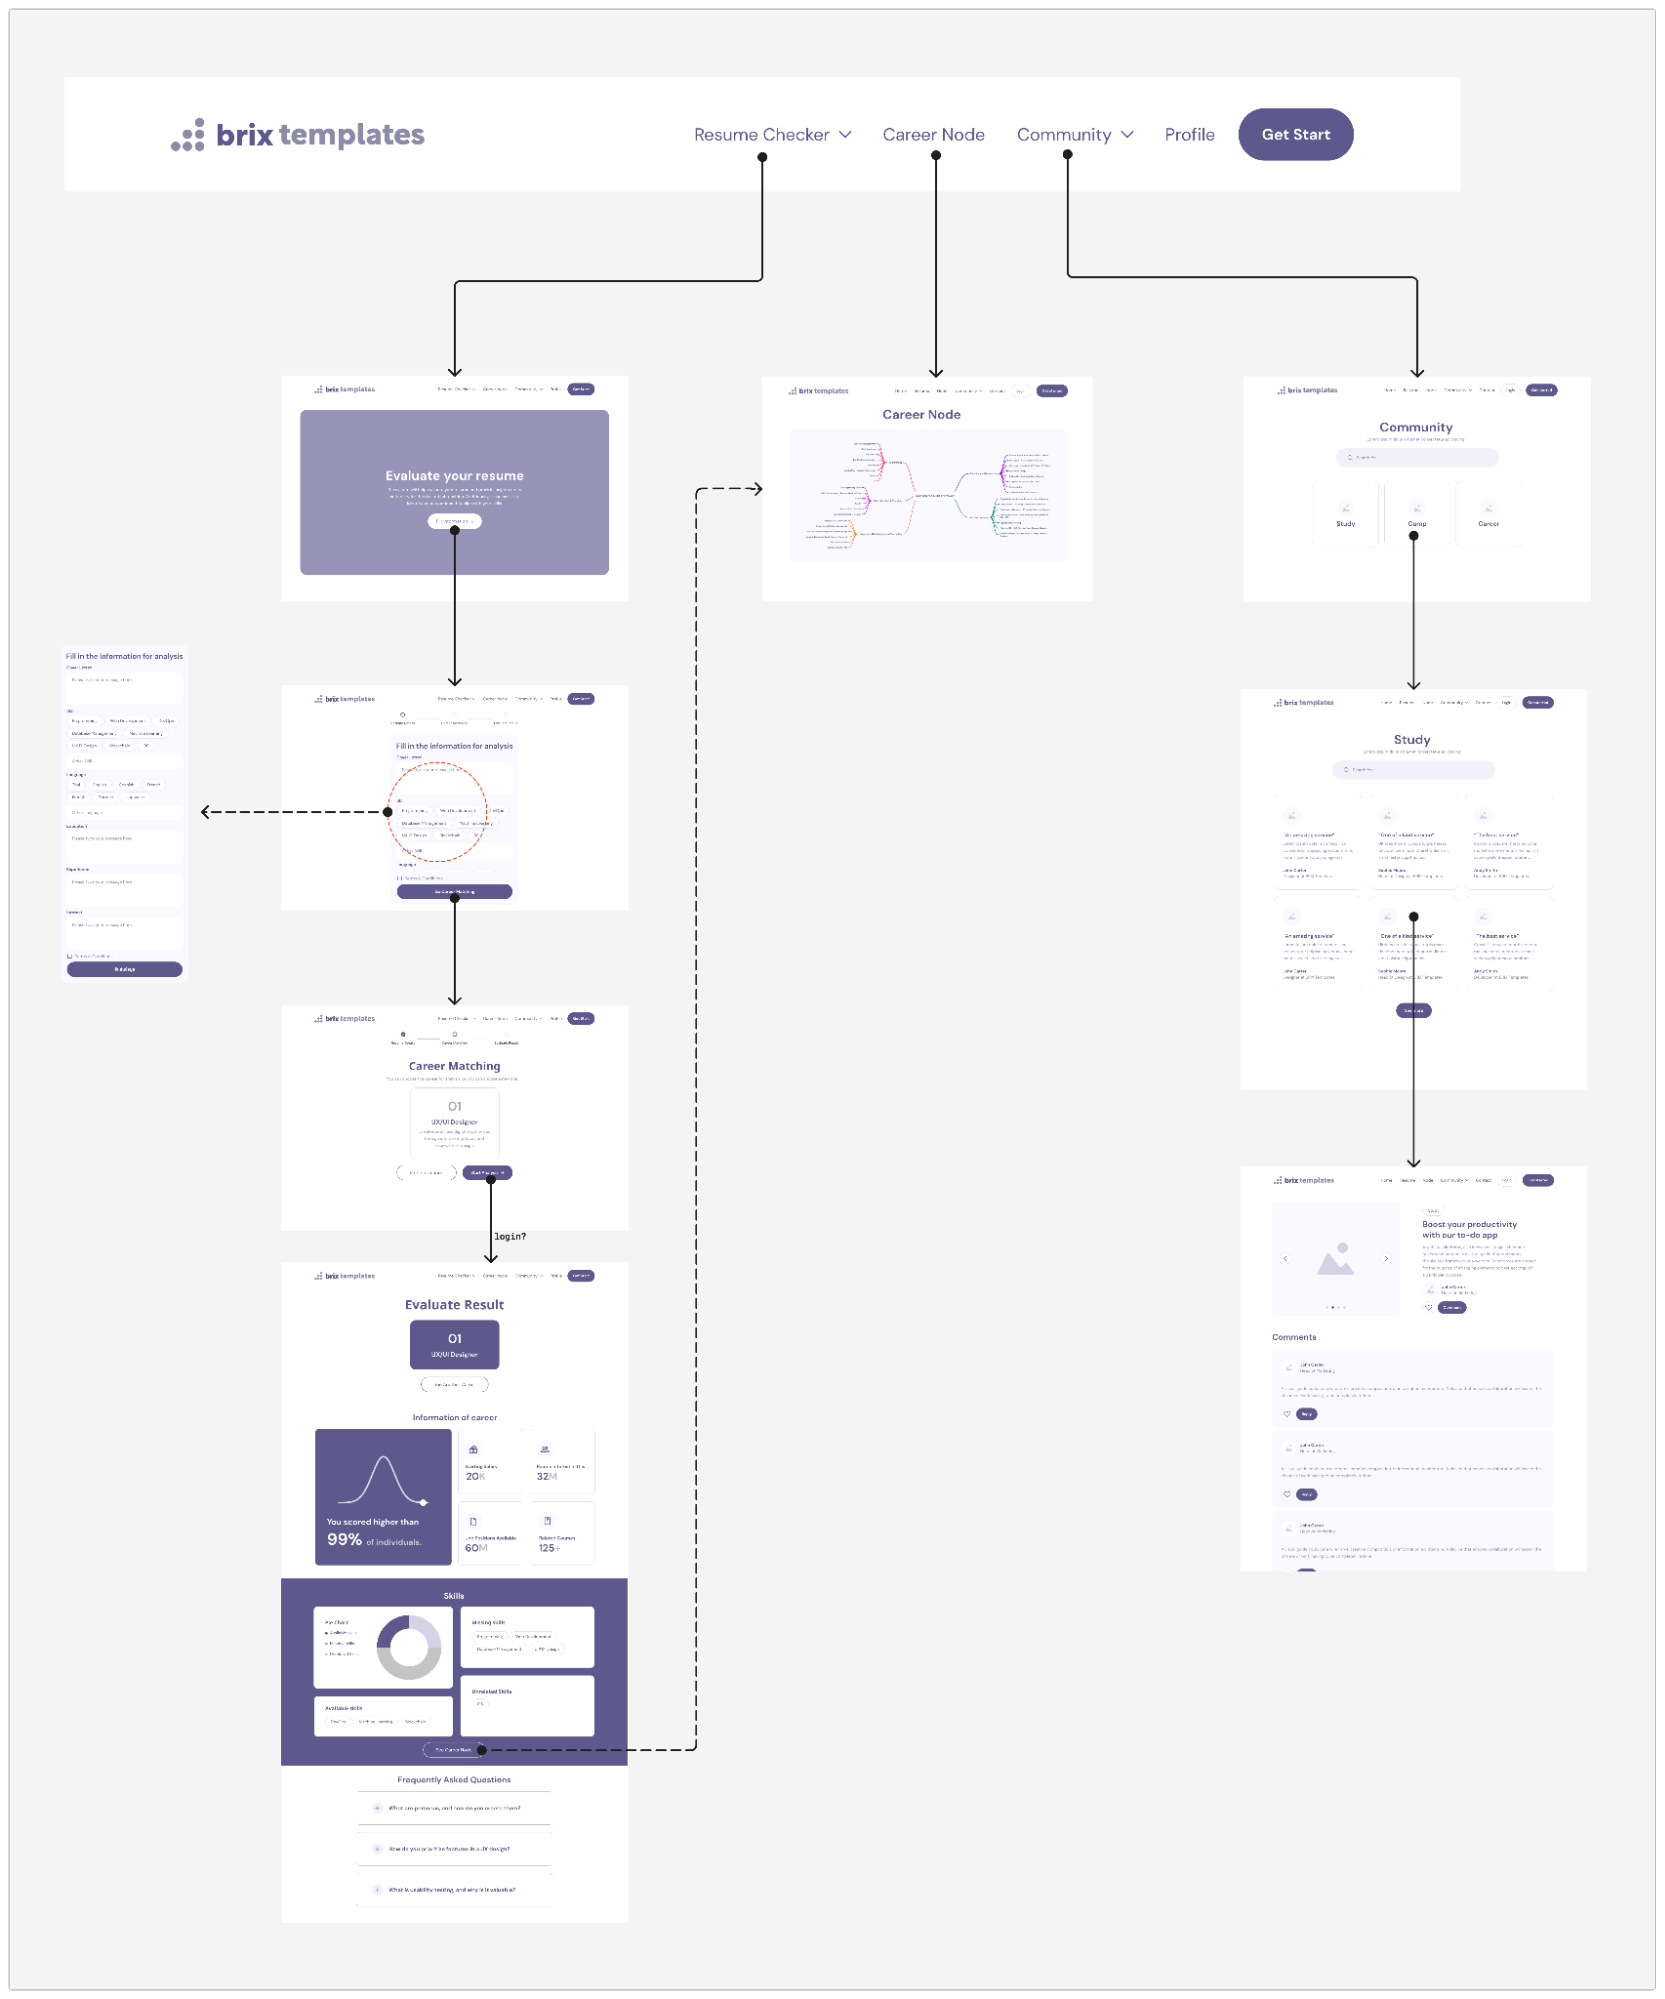
\includegraphics[width=10cm]{./figure/figure_navMap.png}}
    \caption{Navigation Map}\label{fig:navMap}
\end{figure}
\newpage
\section{Wireframe}
การสร้าง wireframe เป็นขั้นตอนสำคัญในกระบวนการออกแบบเว็บหรือแอบพลิเคชัน เนื่องจากช่วยให้ทีมออกแบบและผู้เกี่ยวข้องเข้าใจโครงสร้างพื้นฐานของหน้าจอและการจัดวางองค์ประกอบหลัก ๆ โดยไม่จำเป็นต้องใส่รายละเอียดกราฟิกหรือสี นอกจากนี้ยังช่วยทำให้เห็นถึงภาพรวมประสบการณ์ผู้ใช้
ทำให้สามารถทดสอบและปรับปรุงก่อนที่จะเริ่มการพัฒนา และทำให้กระบวนการออกแบบเป็นไปอย่างมีประสิทธิภาพและรวดเร็วขึ้น โดยเราเลือกที่จะสร้าง wireframe ในส่วนที่เป็นฟีเจอร์สำคัญเพื่อที่จะสามารถนำไปทดสอบกับผู้ใช้ในกระบวนการคิดเชิงออกแบบ (Design Thinking)
\begin{table}[H]
\begin{tabular}{|l|}
\hline
Resume Checker                                                                                                                                                                                                                 \\ \hline
\begin{minipage}{\linewidth}
  \begin{itemize}
    \item หน้าหลัก
  \end{itemize}
\end{minipage}                                                                                                                                                                                                       \\ \hline
 \begin{minipage}{\linewidth}
    \centering
    \vspace{1em} % Adjust the space as needed
  \fbox{
\includegraphics[width=10cm]{./figure/figure_wireframe_table1_mainpage1.png}}
  \caption{\centering หน้าหลักสำหรับกดเริ่มวิเคราะห์ Resume}\label{fig:wireframe1_1}
\end{minipage} \\                          
  \begin{minipage}{\linewidth}
    \centering
    \vspace{1em} % Adjust the space as needed
  \fbox{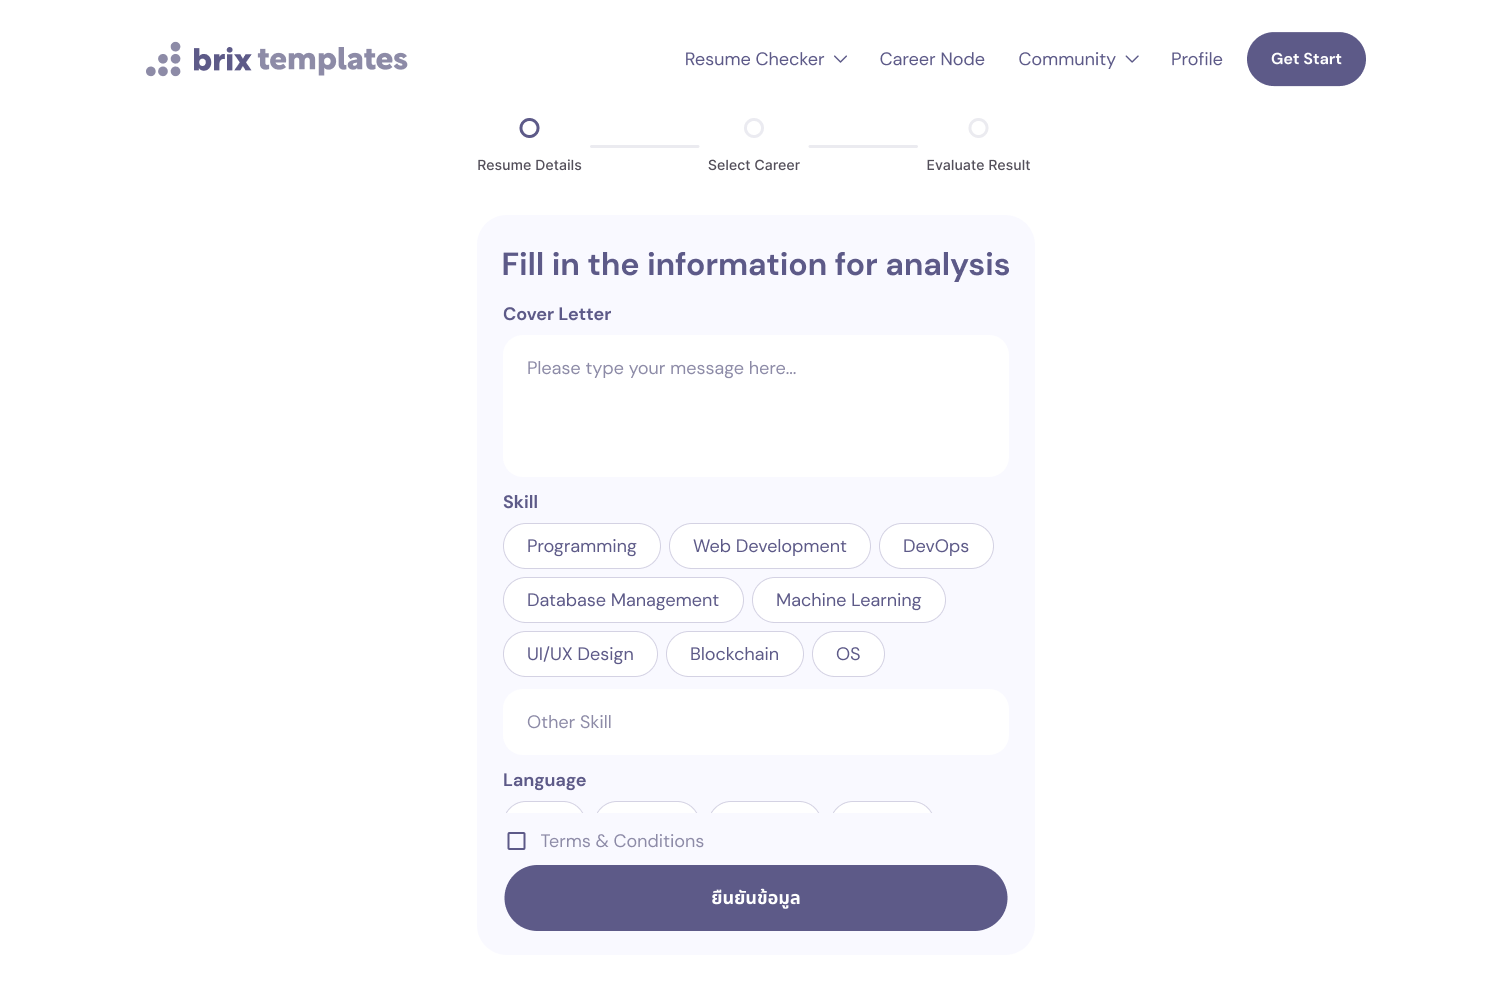
\includegraphics[width=10cm]{./figure/figure_wireframe_table1_mainpage2.png}}
  \caption{\centering หน้ากรอกข้อมูลของเพื่อนำไปวิเคราะห์}\label{fig:wireframe1_2}
\end{minipage} \\                                                                                                                                                                                                                            \\ \hline
\end{tabular}
\end{table}

\begin{table}[H]
\begin{tabular}{|l|}
\hline
\begin{minipage}{\linewidth}
  \begin{itemize}
    \item ส่วนประกอบแบบโต้ตอบ
  \end{itemize}
\end{minipage}                                                                                                                                                                                                               \\ \hline
  \begin{minipage}{\linewidth}
    \centering
    \vspace{1em} % Adjust the space as needed
  \fbox{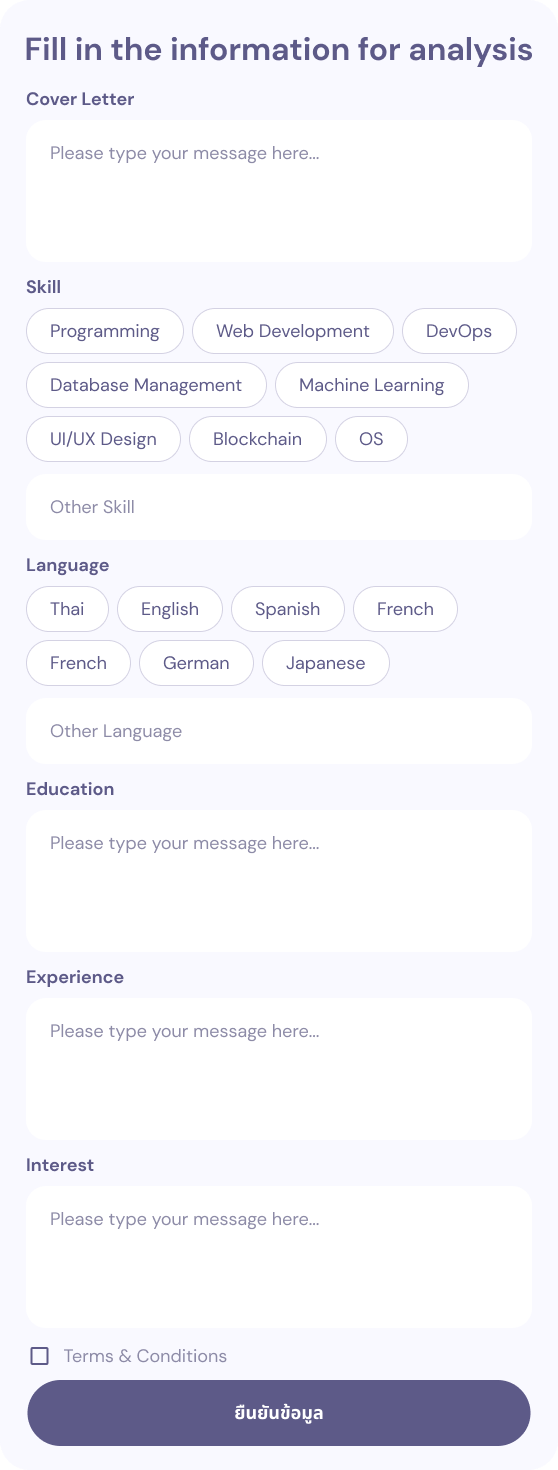
\includegraphics[width=6cm]{./figure/figure_wireframe_table1_component1.png}}
  \caption{\centering ช่องสำหรับกรอกข้อมูลของเพื่อนำไปวิเคราะห์}\label{fig:wireframe1_3}
\end{minipage} \\                                                                                                                                                                                                                                               \\ \hline
\begin{minipage}{\linewidth}
  \begin{itemize}
    \item คำอธิบาย
  \end{itemize}
\end{minipage}                                                                                                                                                                                                                       \\ \hline
\begin{minipage}{\linewidth}
  \raggedright
  Resume Checker เป็นฟีเจอร์ที่ให้ผู้ใช้กรอกข้อมูลของเพื่อนำไปวิเคราะห์อาชีพที่เหมาะสม โดยผู้ใช้สามารถการข้อมูลเกี่ยวกับประสบการณ์ทำงาน, การศึกษา, ทักษะ, และคุณสมบัติอื่น ๆ ที่สำคัญ
\end{minipage}
 \\ \hline
\end{tabular}
\end{table}


\begin{table}[H]
\begin{tabular}{|l|}
\hline
Match Career                                                                                                                                                                                                                                                                                                    \\ \hline
\begin{minipage}{\linewidth}
  \begin{itemize}
    \item หน้าหลัก
  \end{itemize}
\end{minipage}                                                                                                                                                                                                                                                                                                 \\ \hline
   \begin{minipage}{\linewidth}
    \centering
    \vspace{1em} % Adjust the space as needed
  \fbox{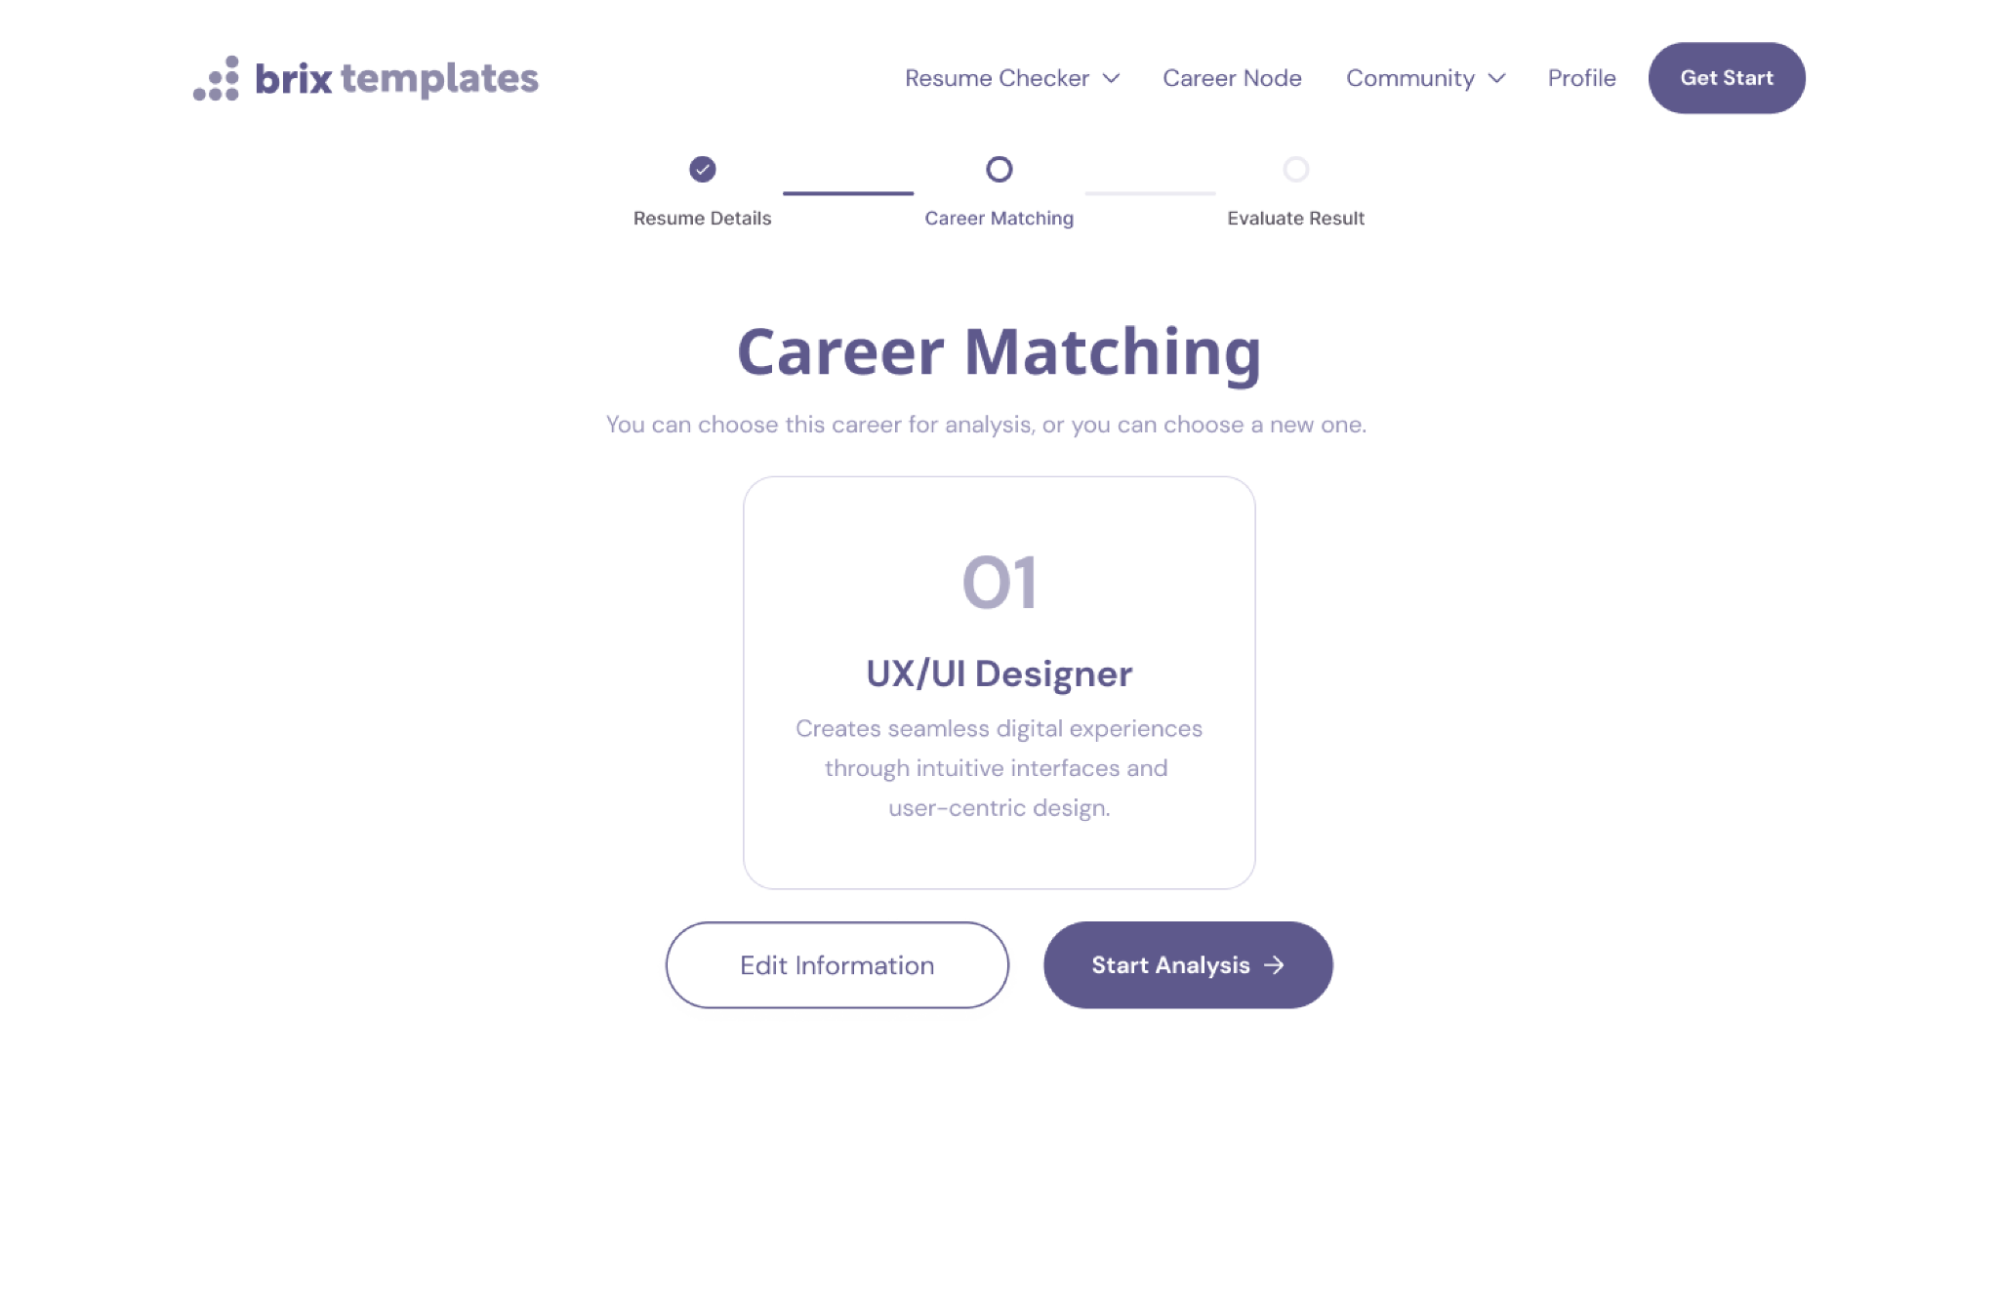
\includegraphics[width=10cm]{./figure/figure_wireframe_table2_mainpage1.png}}
  \caption{\centering หน้าแสดงอาชีพที่วิเคราะห์ได้}\label{fig:wireframe2_1}
\end{minipage} \\                                                                                                                                                                                                                                                                                                                                   \\ \hline
\begin{minipage}{\linewidth}
  \begin{itemize}
    \item คำอธิบาย
  \end{itemize}
\end{minipage}                                                                                                                                                                                                                                                                                                                                                                                                                                                                                                                                 \\ \hline
\begin{minipage}{\linewidth}
  \raggedright
Match Career เป็นฟีเจอร์สำหรับแสดงอาชีพที่เหมาะสมกับข้อมูลที่ผู้ใช้กรอกมาทำให้ผู้ใช้สามารถรู้ถึงอาชีพที่เหมาะสมกับตนเองและข้อมูลคร่าว ๆ ของอาชีพนั้น โดยผู้ใช้สามารถกลับไปแก้ไขข้อมูลที่กรอกได้เพื่อนำมาวิเคราะห์อาชีพใหม่ รวมถึงสามารถกดวิเคราะห์ข้อมูลเชิงลึกต่อไปได้แต่ผู้ใช้ต้องสมัครและล็อคอินเพื่อเก็บข้อมูลก่อน
\end{minipage}
\\ \hline
\end{tabular}
\end{table}

\begin{table}[H]
\begin{tabular}{|l|}
\hline
Evaluate Result                                                                                                                                                                                                                                                                                                   \\ \hline
\begin{minipage}{\linewidth}
  \begin{itemize}
    \item หน้าหลัก
  \end{itemize}
\end{minipage}                                                                                                                                                                                                                                                                                                                      \\ \hline
  \begin{minipage}{\linewidth}
    \centering
    \vspace{1em} % Adjust the space as needed
  \fbox{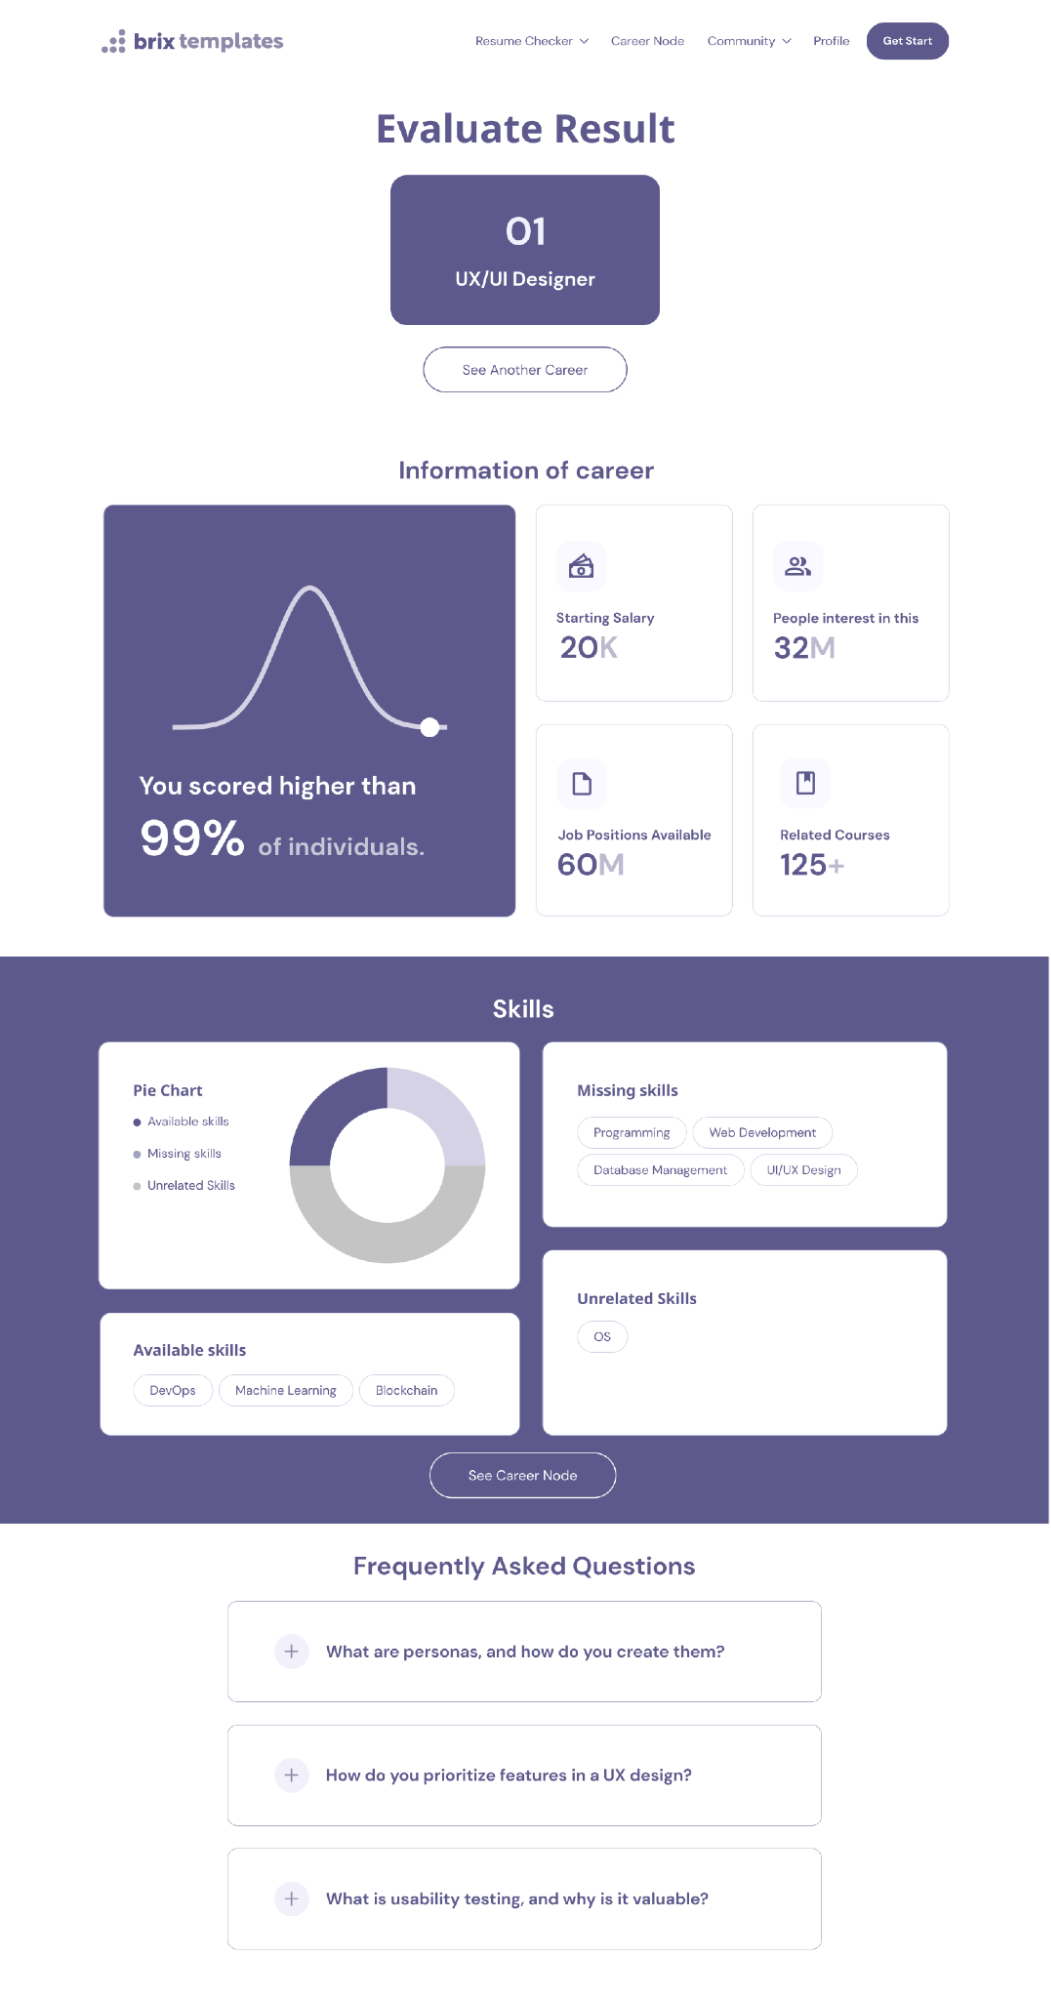
\includegraphics[width=10cm]{./figure/figure_wireframe_table3_mainpage1.png}}
  \caption{\centering หน้าแสดงข้อมูลเชิงลึกของอาชีพ}\label{fig:wireframe3_1}
\end{minipage} \\                                                                                                                                                                                                                                                                                                                                    \\ \hline
\begin{minipage}{\linewidth}
  \begin{itemize}
    \item คำอธิบาย
  \end{itemize}
\end{minipage}                                                                                                                                                                                                                                                                                                                                                                                                                                                                                                                                 \\ \hline
\begin{minipage}{\linewidth}
  \raggedright
Evaluate Result เป็นฟีเจอร์สำหรับแสดงข้อมูลเชิงลึกของอาชีพที่วิเคราะห์ได้ในตอนแรก โดยจะแสดงข้อมูลที่มีโยชน์เพื่อให้ผู้ใช้สามารถนำไปพัฒนาทักษะของตนเองและเรูเม่ต่อไปได้
\end{minipage}
\\ \hline
\end{tabular}
\end{table}

\begin{table}[H]
\begin{tabular}{|l|}
\hline
Career Node                                                                                                                                                                                                                                                                                              \\ \hline
\begin{minipage}{\linewidth}
  \begin{itemize}
    \item หน้าหลัก
  \end{itemize}
\end{minipage}                                                                                                                                                                                                                                                                                                                 \\ \hline
 \begin{minipage}{\linewidth}
    \centering
    \vspace{1em} % Adjust the space as needed
  \fbox{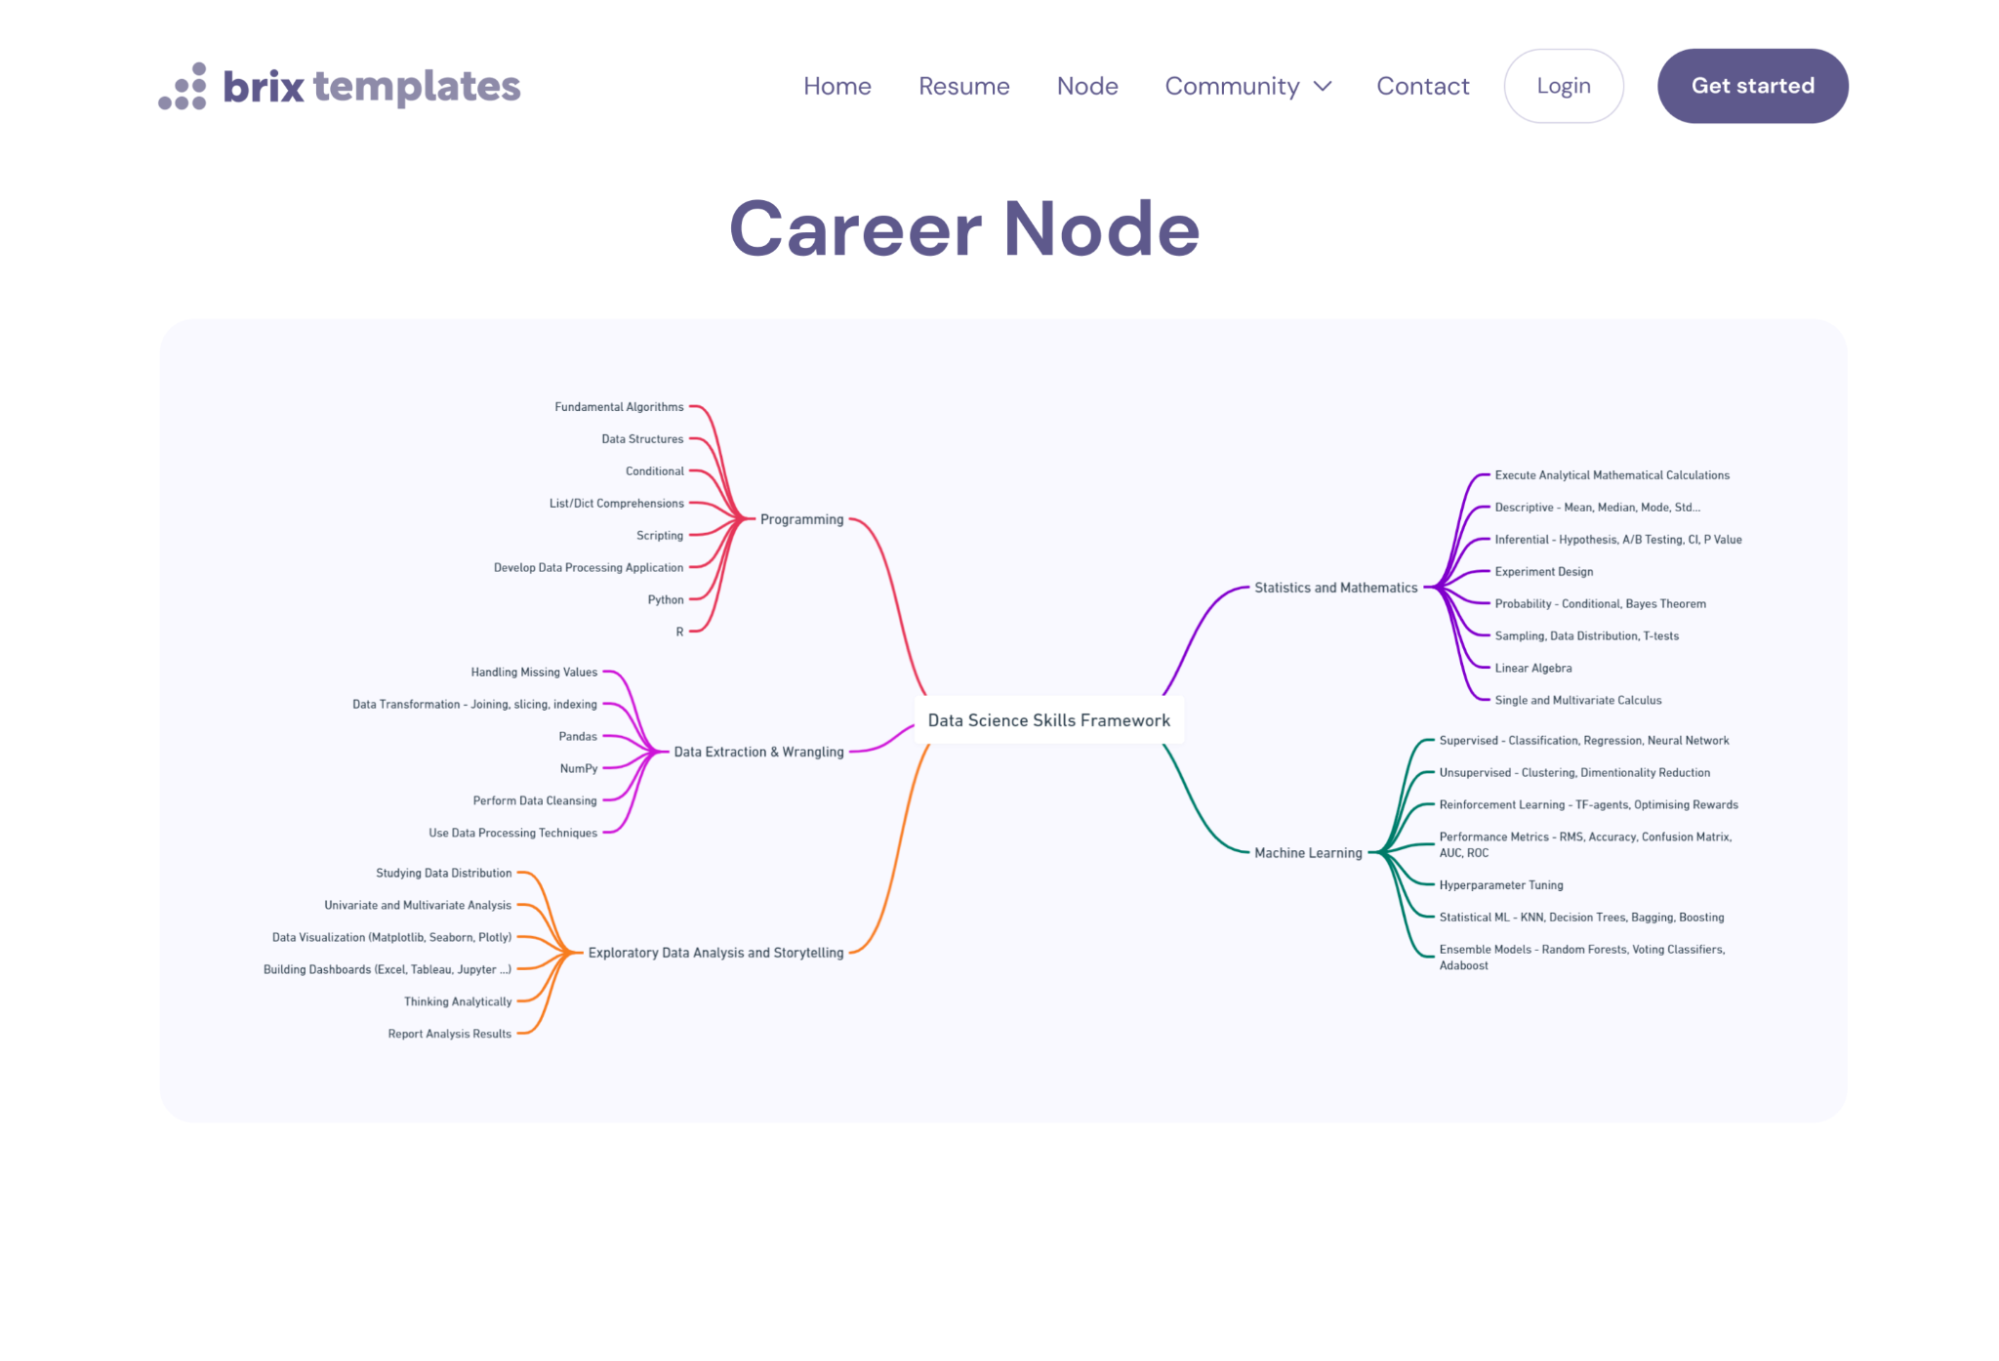
\includegraphics[width=10cm]{./figure/figure_wireframe_table4_mainpage1.png}}
  \caption{\centering หน้าแสดงทักษะที่ใช้ในสายอาชีพ}\label{fig:wireframe4_1}
\end{minipage} \\                                                                                                                                                                                                                                                                                                                                                    \\ \hline
\begin{minipage}{\linewidth}
  \begin{itemize}
    \item คำอธิบาย
  \end{itemize}
\end{minipage}                                                                                                                                                                                                                                                                                                                                                                                                                                                                                                                            \\ \hline
\begin{minipage}{\linewidth}
  \raggedright
Career Node เป็นฟีเจอร์สำหรับแสดงทักษะที่ต้องใช้ในอาชีพต่าง ๆ โดยจะแสดงออกมาในรูปแบบโหนด
\end{minipage}
\\ \hline
\end{tabular}
\end{table}

\begin{table}[H]
\begin{tabular}{|l|}
\hline
Community                                                                                                                                                                                                                                                                                          \\ \hline
\begin{minipage}{\linewidth}
  \begin{itemize}
    \item หน้าหลัก
  \end{itemize}
\end{minipage}                                                                                                                                                                                                                                                                                                                        \\ \hline
 \begin{minipage}{\linewidth}
    \centering
    \vspace{1em} % Adjust the space as needed
  \fbox{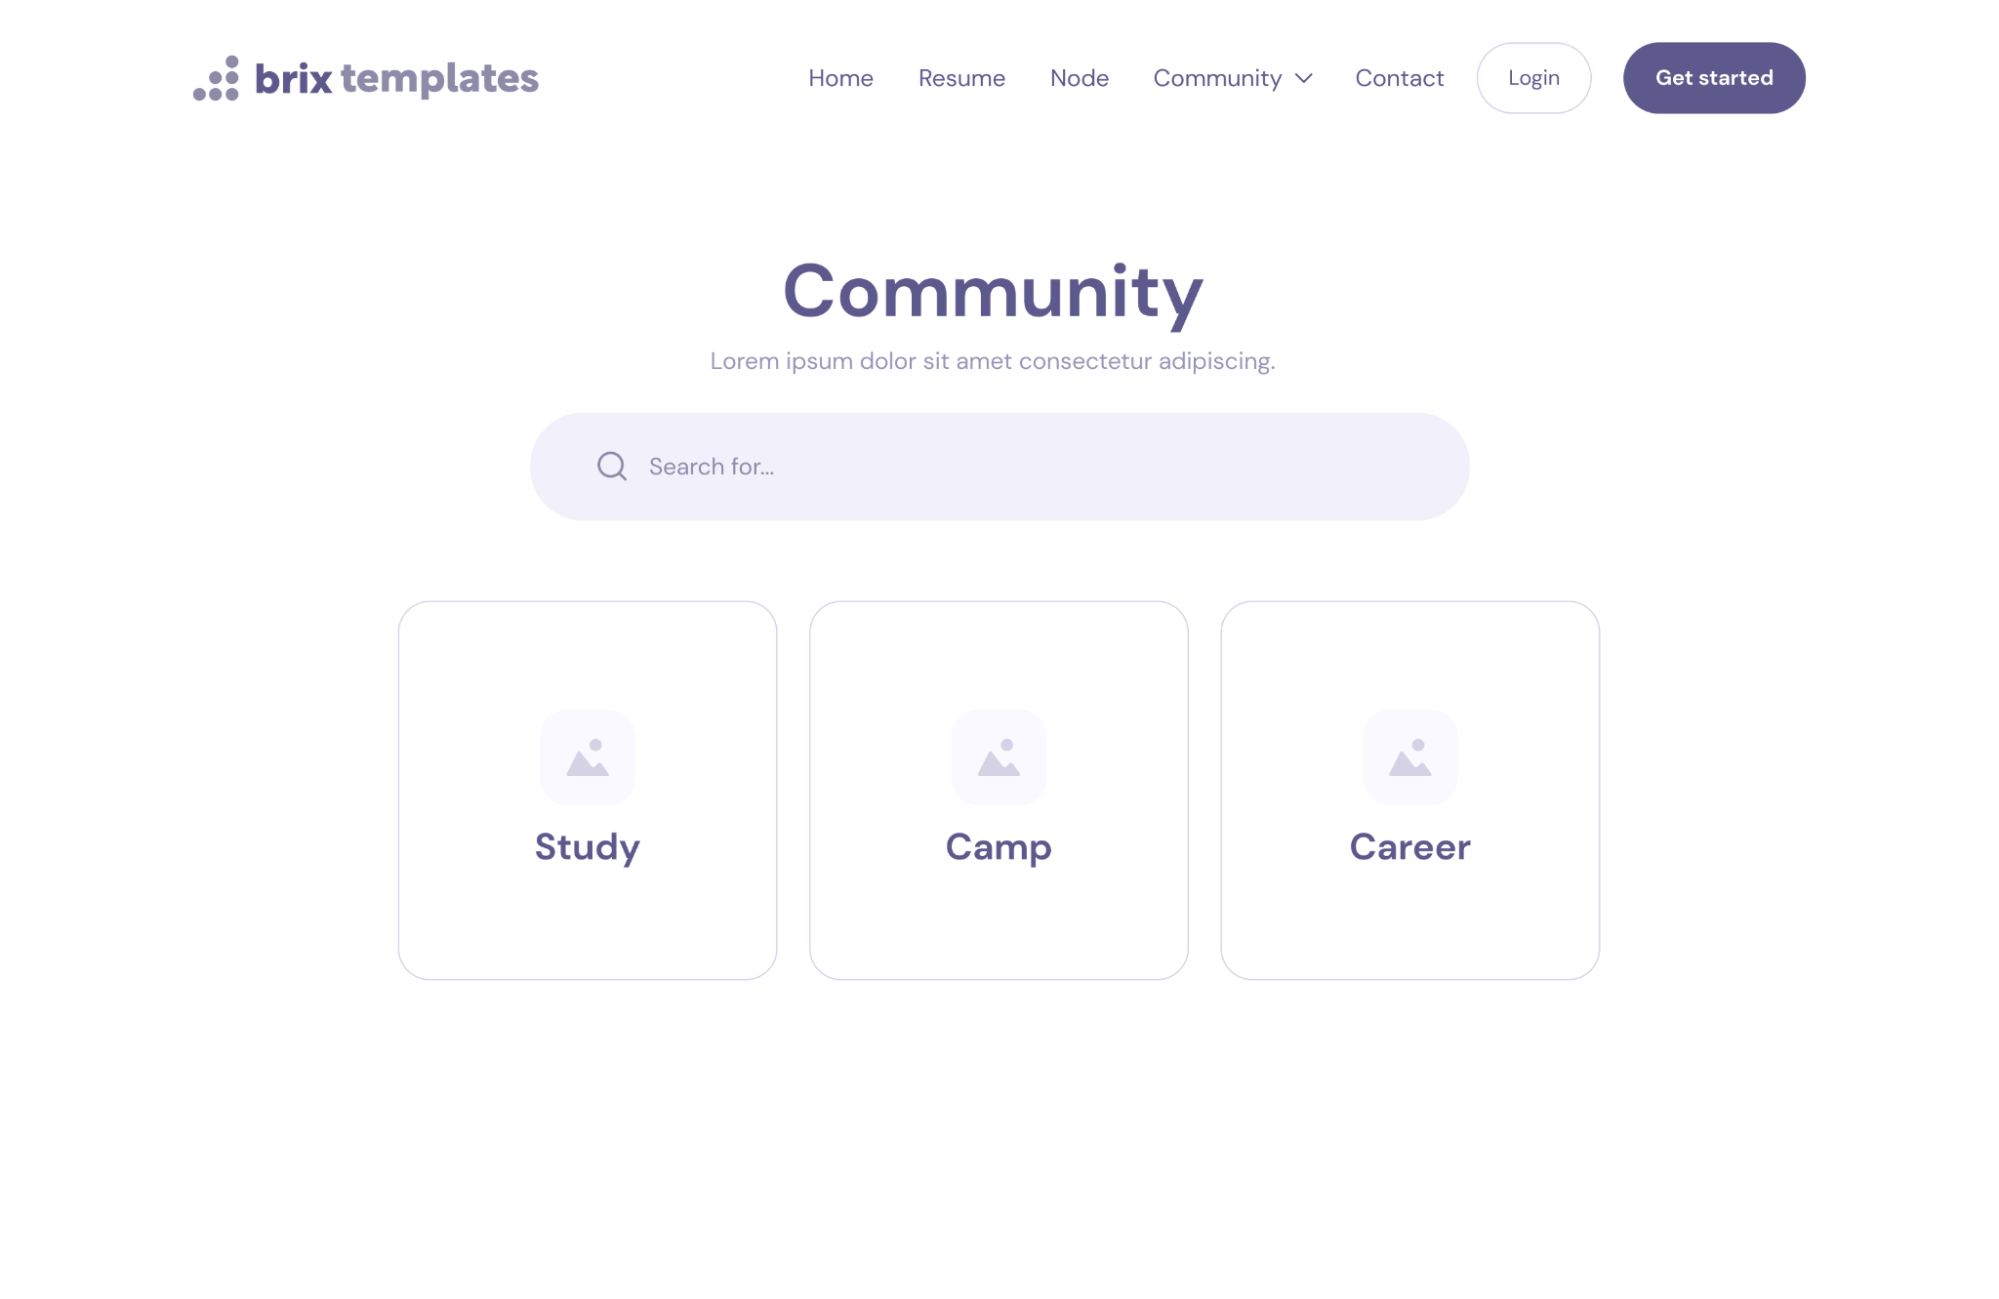
\includegraphics[width=10cm]{./figure/figure_wireframe_table5_mainpage1.png}}
  \caption{\centering หน้าเลือกหมวดหมู่กของกระทู้}\label{fig:wireframe5_1}
\end{minipage} \\       
 \begin{minipage}{\linewidth}
    \centering
    \vspace{1em} % Adjust the space as needed
  \fbox{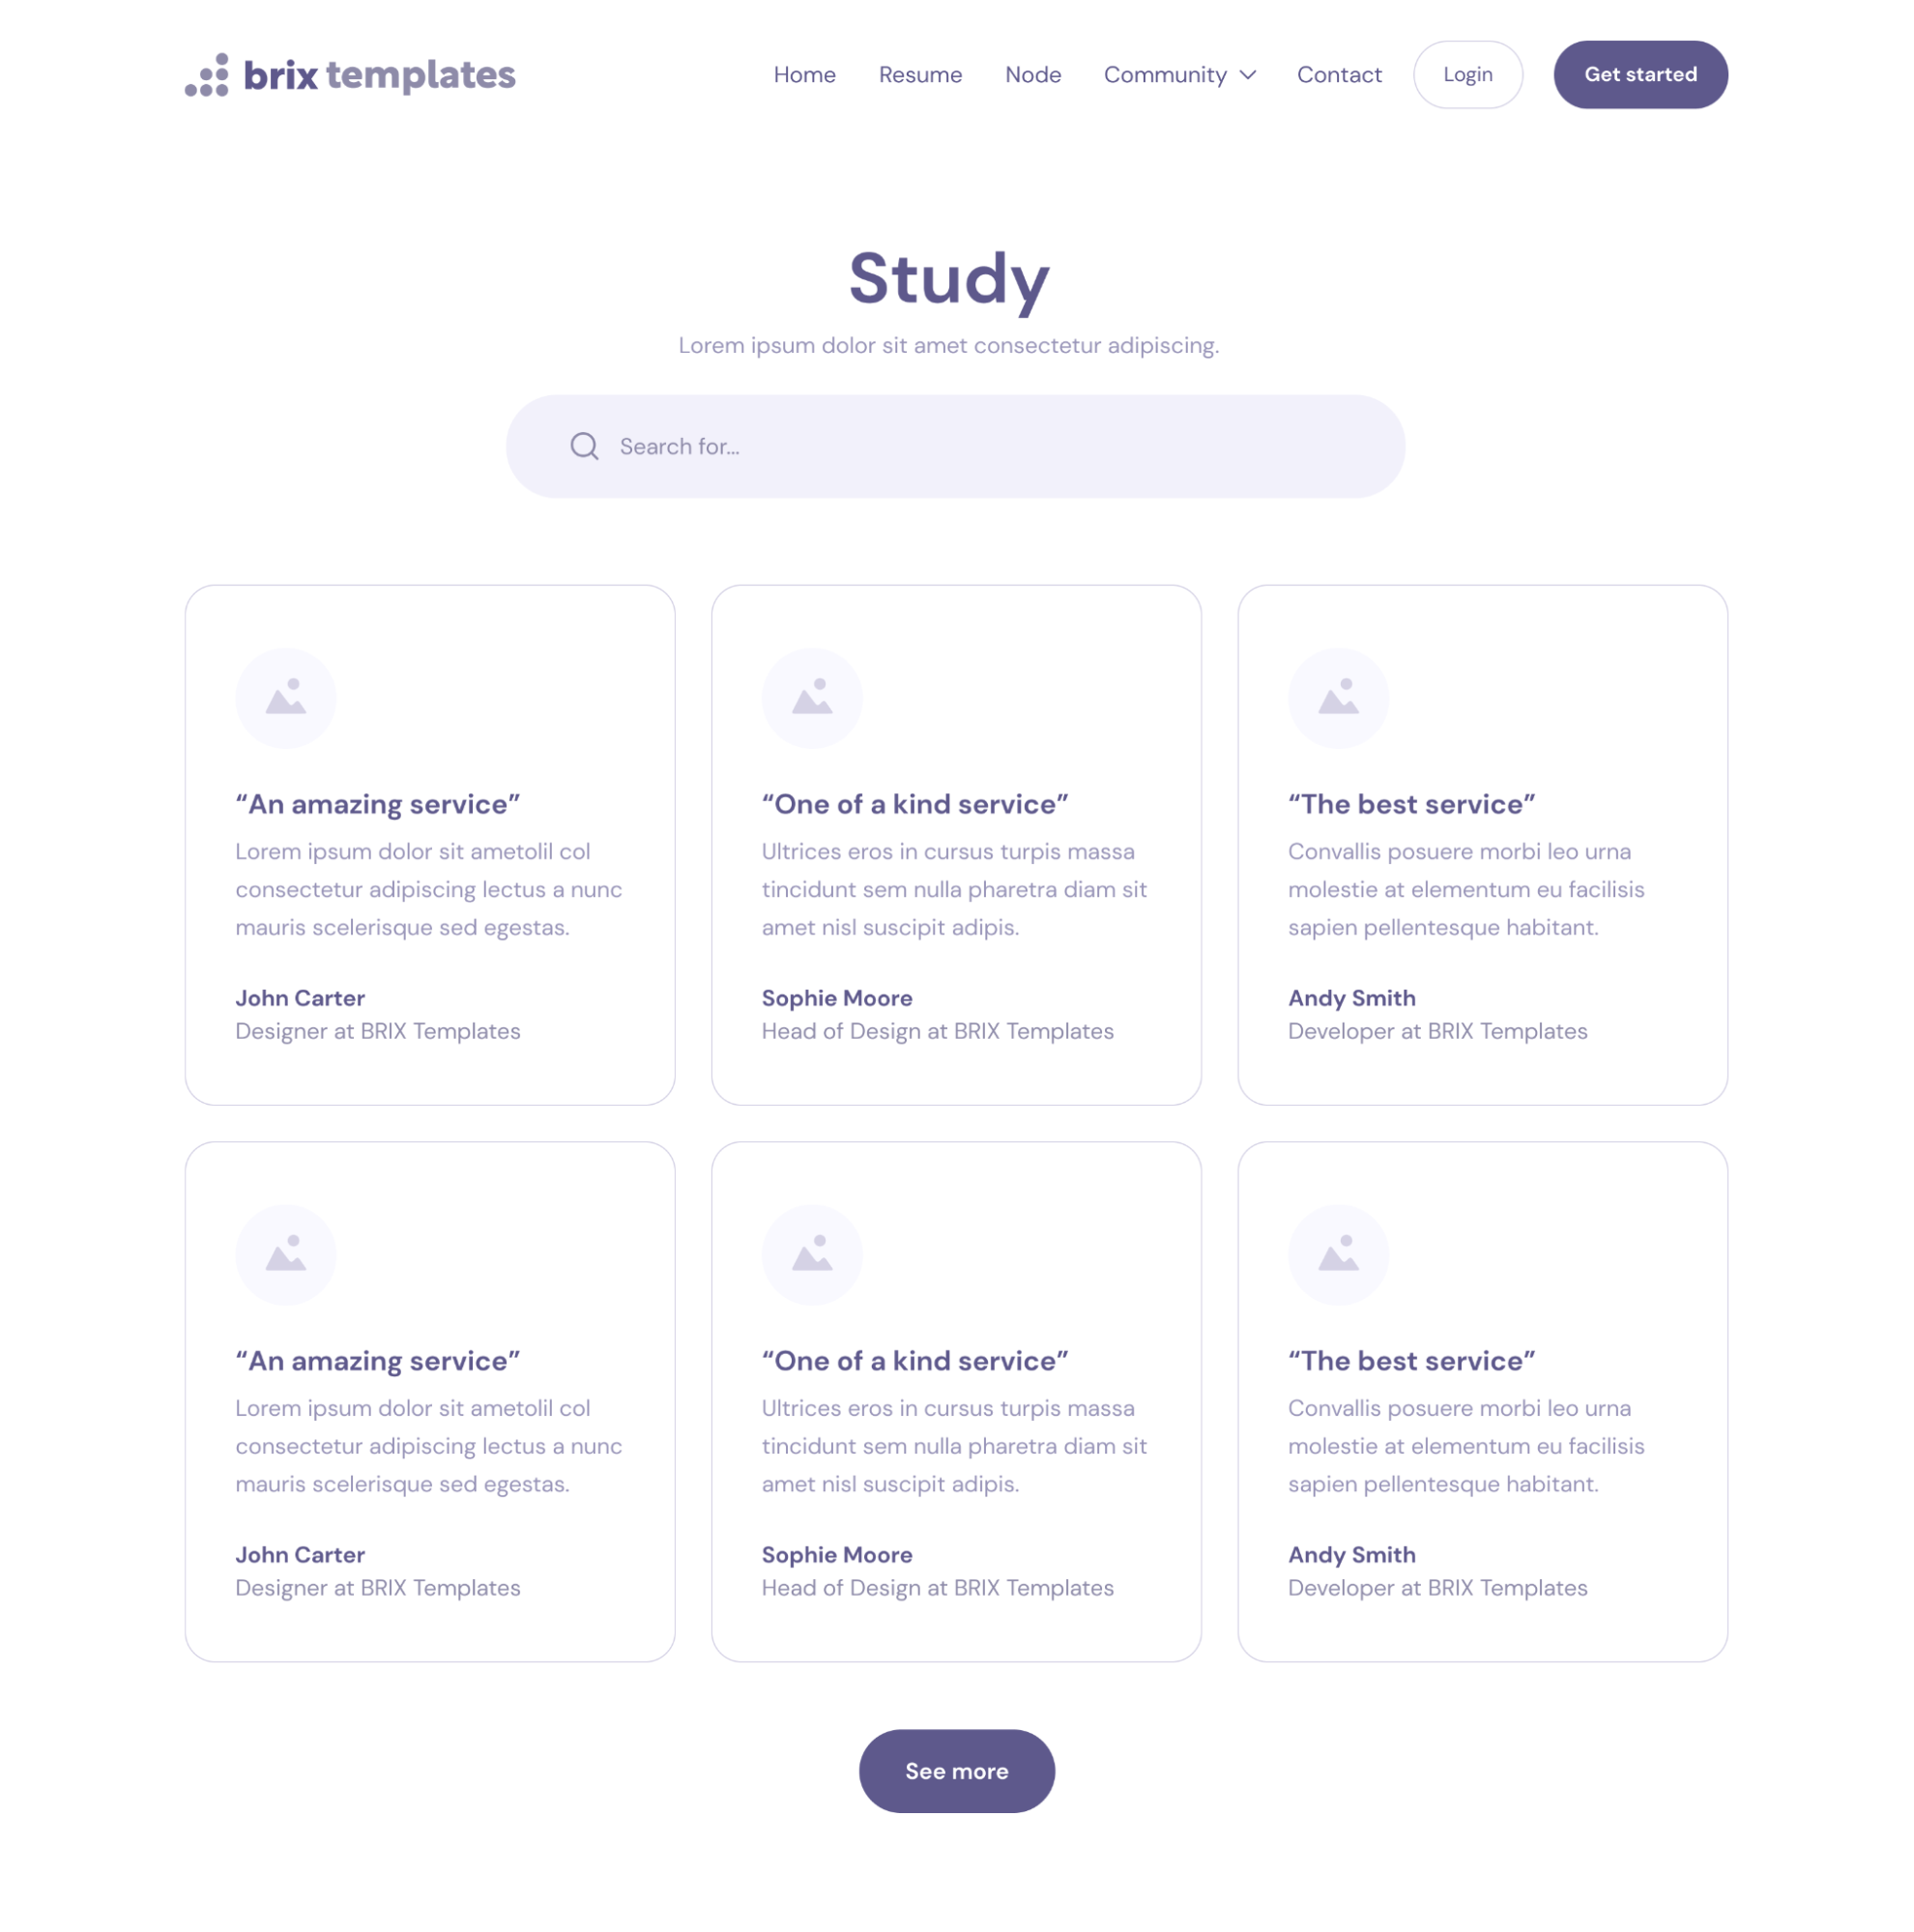
\includegraphics[width=10cm]{./figure/figure_wireframe_table5_mainpage2.png}}
  \caption{\centering หน้าแสดงรายการกระทู้}\label{fig:wireframe5_2}
\end{minipage} \\                           
\\ \hline
\end{tabular}
\end{table}

\begin{table}[H]
\begin{tabular}{|l|}
\hline
\begin{minipage}{\linewidth}
    \centering
    \vspace{1em} % Adjust the space as needed
  \fbox{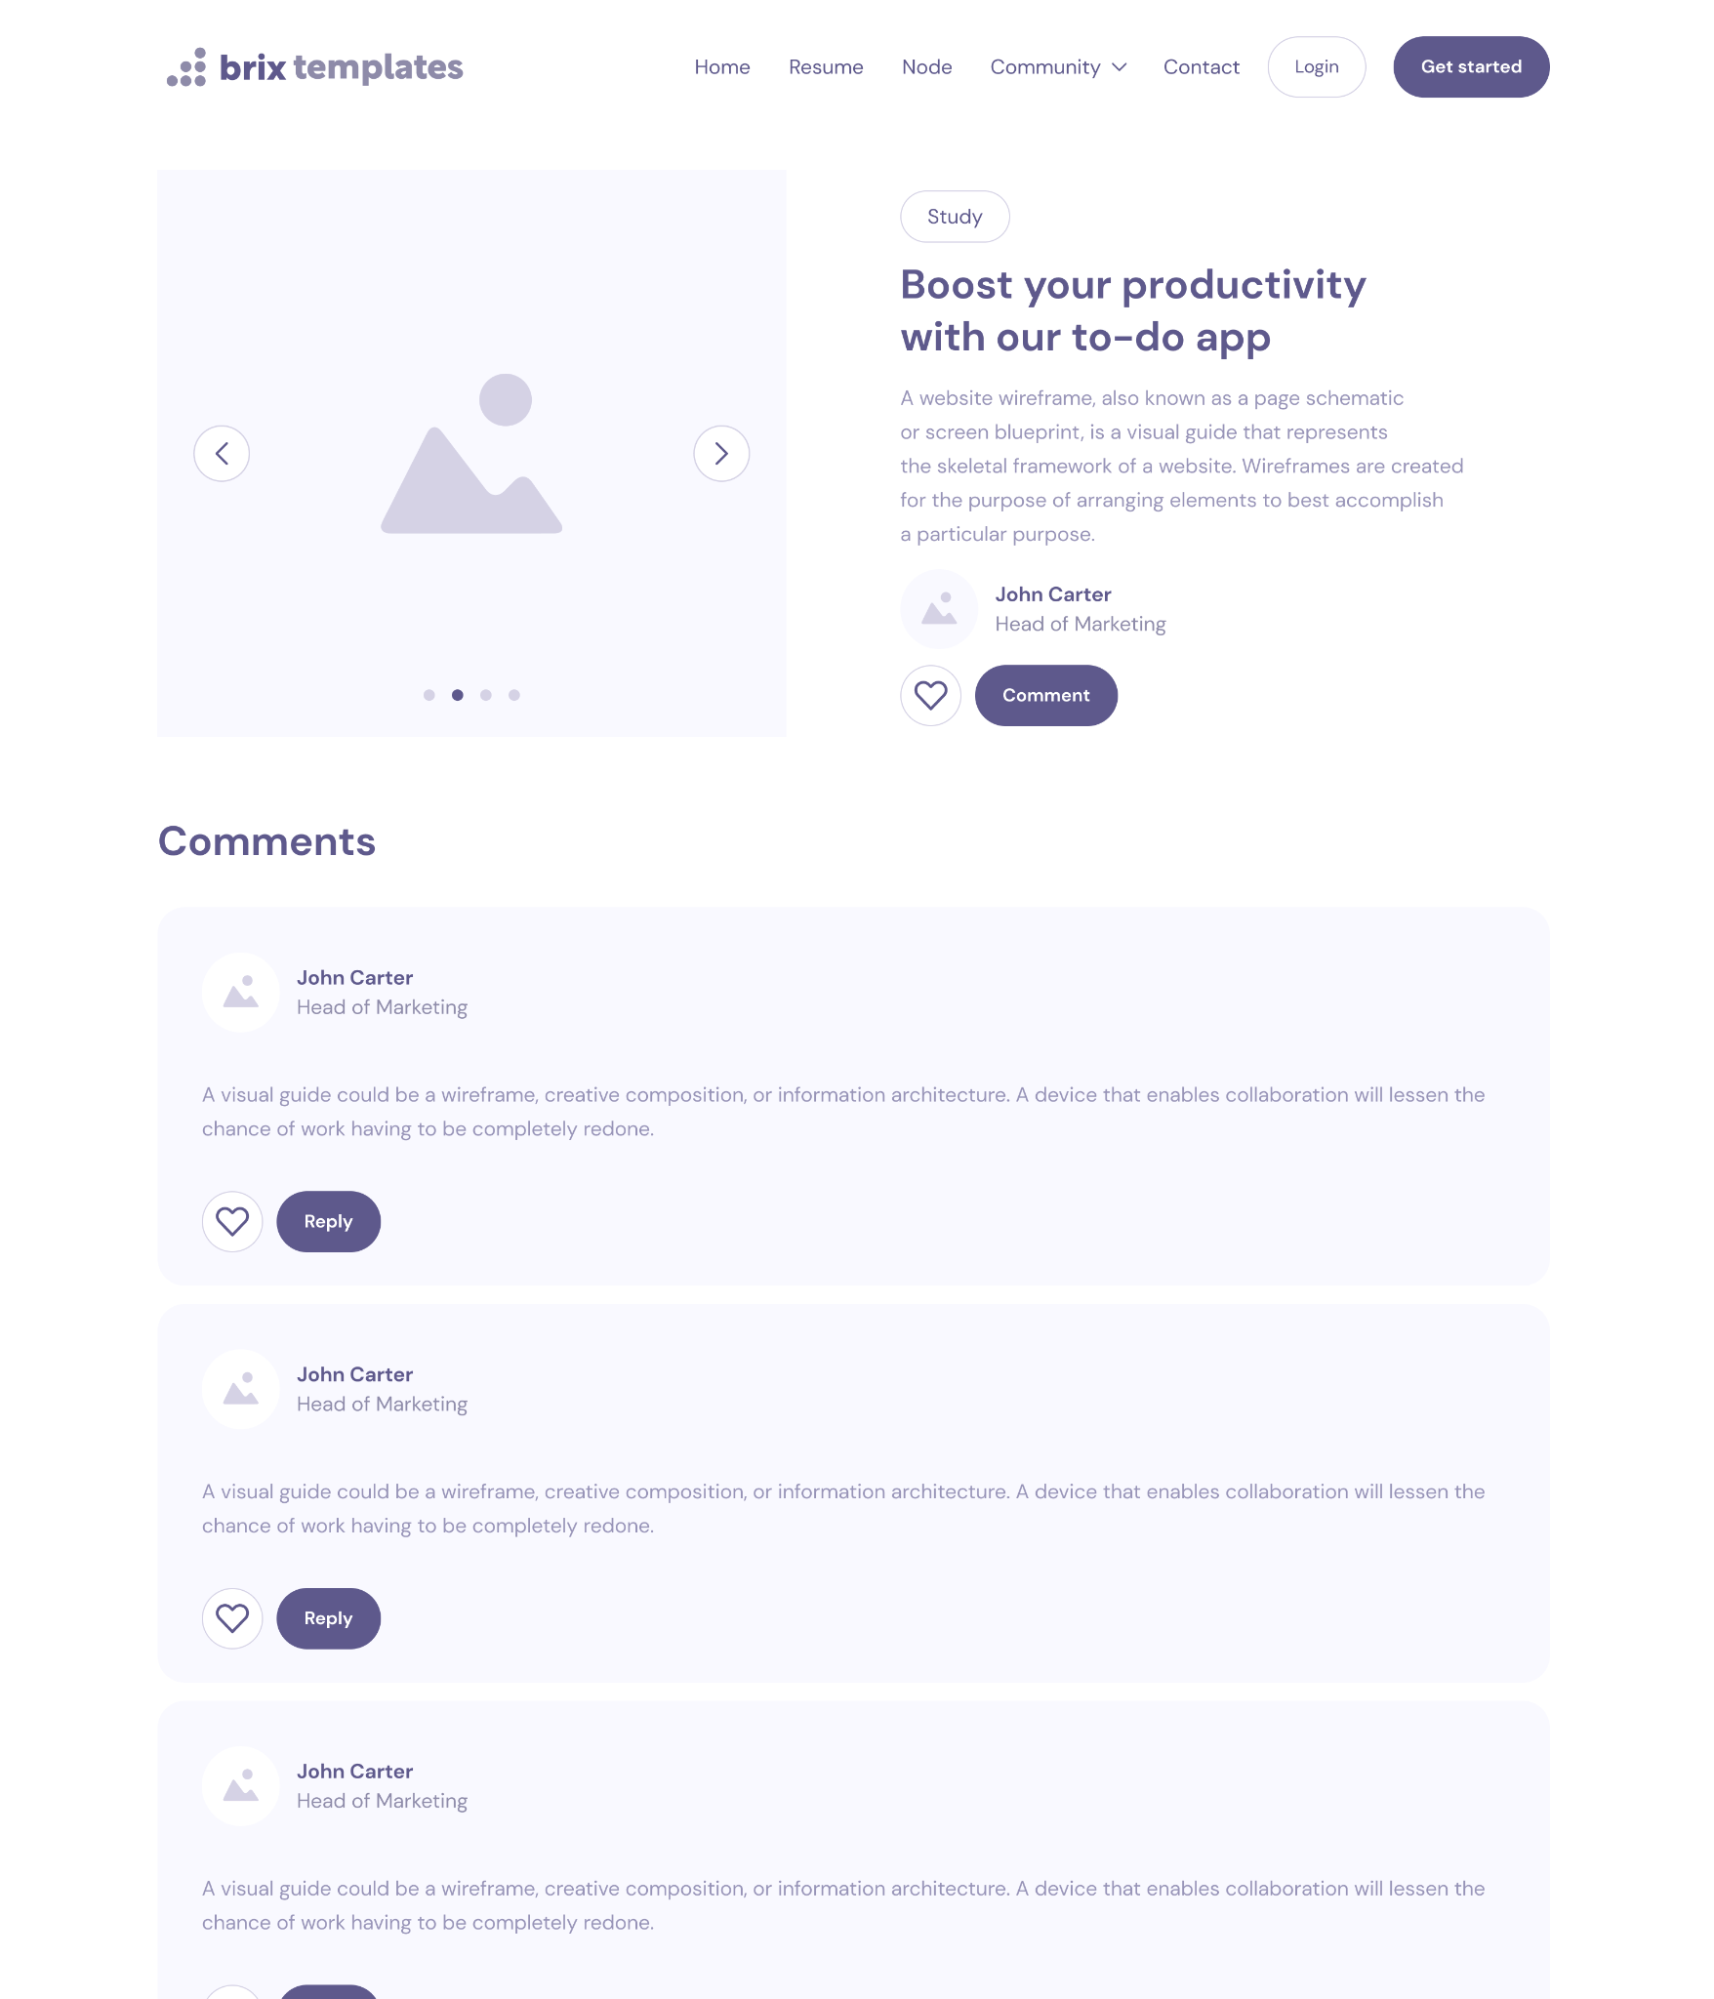
\includegraphics[width=10cm]{./figure/figure_wireframe_table5_mainpage3.png}}
  \caption{\centering หน้าแสดงรายละเอียดของกระทู้}\label{fig:wireframe5_3}
\end{minipage} \\                                                                                                                                                                                                                                                                                                       \\ \hline
\begin{minipage}{\linewidth}
  \begin{itemize}
    \item คำอธิบาย
  \end{itemize}
\end{minipage}                                                                                                                                                                                                                                                                                            \\ \hline
\begin{minipage}{\linewidth}
  \raggedright
Community เป็นฟีเจอร์สำหรับให้ผู้ใช้สามารถเข้ามาแลกเปลี่ยนข้อมูลหรือความคิดเห็นได้ผ่านการตั้งกระทู้และแสดงความคิดเห็น
\end{minipage}
\\ \hline
\end{tabular}
\end{table}


\section{ขั้นตอนการพัฒนาโมเดล}
\subsection{การรวบรวมข้อมูล (Get Data)}
ทางคณะผู้จัดทำได้เลือกนำชุดข้อมูล Updated Resume Dataset \cite{dataset} จาก Kaggle ซึ่งเป็นชุดข้อมูล
ที่ประกอบไปด้วยอาชีพทั้งหมด 25 หมวด และรายละเอียดภายในเรซูเมของแต่ละอันที่จะแตกต่างกันไปในแต่ละอัน ซึ่งมีเรซูเม
ทั้งหมด 962 เล่ม
\begin{figure}[h]\centering
    \setlength{\fboxrule}{0.2mm} % can define this in the preamble
    \setlength{\fboxsep}{0.5cm}
    \fbox{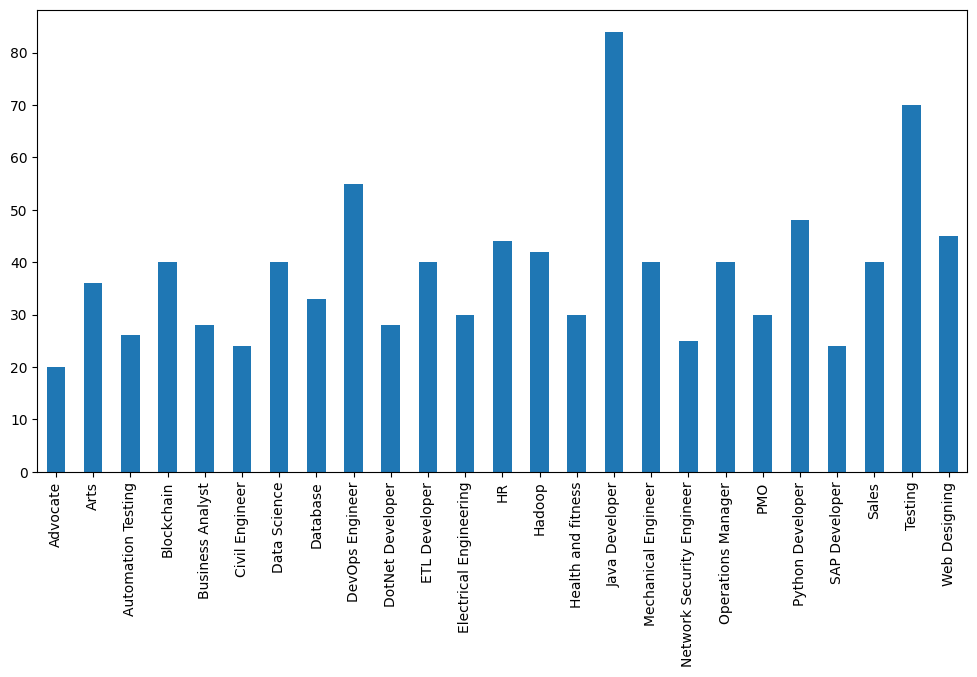
\includegraphics[width=10cm]{./figure/figure_datasetCategory.png}}
    \caption{จำนวนของเรซูเมในแต่ละหมวดอาชีพ}\label{fig:datasetCategory}
\end{figure}
\begin{figure}[h]\centering
    \setlength{\fboxrule}{0.2mm} % can define this in the preamble
    \setlength{\fboxsep}{0.5cm}
    \fbox{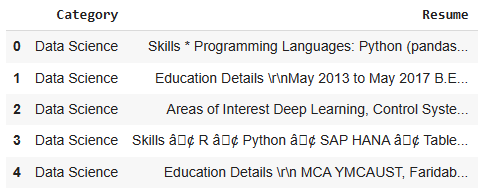
\includegraphics[width=10cm]{./figure/figure_datasetData.png}}
    \caption{ลักษณะข้อมูลของชุดข้อมูล}\label{fig:datasetData}
\end{figure}
\par ซึ่งทางคณะผู้จัดทำ จำเป็นต้องทำการเตรียมข้อมูลที่เหมาะสมเพื่อให้โมเดลมีประสิทธิภาพ

\subsection{การเตรียมข้อมูล (Clean, Prepare and Manipulate Data)}
หลังจากที่ทางคณะผู้จัดทำได้ทำการสำรวจชุดข้อมูล ทำให้พบว่ารายละเอียดของเรซูเมยังไม่สามารถนำไปใช้ได้ทันที
เนื่องจากข้อมูลเรซูเม ได้มีตัวอักษรพิเศษรวมอยู่เป็นจำนวนมาก เช่น \^a, €, ¢, \textbackslash r, \textbackslash n
รวมไปถึงมีการใส่ลิงก์ภายนอกอีกด้วย ทางคณะผู้จัดทำจึงจำเป็นที่จะต้องทำให้ตัวหนังสือภายในเรซูเม เป็นเพียงตัวอักษรปกติเท่านั้น
\par เนื่องจากทางคณะผู้จัดทำเล็งเห็นกลุ่มเป้าหมายเป็นนักศึกษาวิศวกรรมคอมพิวเตอร์ มจธ. จึงจำเป็นที่ต้องเลือกเฉพาะข้อมูลที่เป็น
Software Engineer, Designer, Data, Security, Cloud Management ซึ่งเราจำเป็นที่จะต้อง
ลบบางหมวดอาชีพ และทำการรวมบางอาชีพเข้าด้วยกัน
\par และเพื่อให้โมเดลสามารถที่จะเข้าใจภาษาของมนุษย์ได้ คณะผู้จัดทำจึงได้ใช้อัลกอริทึมในการแปลผลภาษา
Term Frequency Inverse Document Frequency (TF-IDF)

\subsection{การเทรนโมเดล (Train Model)}
หลังจากที่ทางคณะผู้จัดทำได้ทำการเตรียมข้อมูลสำเร็จแล้ว คณะผู้จัดทำก็ได้ทำโมเดลขึ้นมาทั้งหมด 2 โมเดลเพื่อเปรียบเทียบ
ซึ่งเป็นโมเดลสำหรับการจัดหมวดหมู่ ได้แก่
\begin{enumerate}
    \item Navie Bayes Classification
    \item Long Short Term Memory (LSTM)
    \begin{itemize}
        \item Embedding layer              | max input dimension is 10,000 and embedding dimension size is 100
        \item Bidirectional LSTM 128 units | dropout rate 40\%
        \item Bidirectional LSTM 64 units  | dropout rate 40\%
        \item Dense layer 25 units         | softmax as activation function
    \end{itemize}
\end{enumerate}
\par และคณะผู้จัดทำก็ทำการใส่ข้อมูลที่เตรียมเอาไว้เพื่อทำการเทรนโมเดล โดยที่โมเดลจะทำการทำนายว่าข้อมูลเรซูเมที่ใส่เข้าไป
เป็นอาชีพใดจากทั้งหมด 5 อาชีพ (Software Engineer, Designer, Data, Security, Cloud Management) ซึ่ง
สามารถแสดงผลออกมาเป็นความน่าจะเป็นของแต่ละสายอาชีพได้

\subsection{การทดสอบข้อมูล (Test Data)}
หลังจากที่คณะผู้จัดทำได้เทรนโมเดลจนสำเร็จแล้ว ก็ได้ลองนำเรซูเมของคณะผู้จัดทำมาลองกับโมเดล ซึ่งผลลัพธ์ที่ได้ก็ค่อนข้างน่าพอใจ
คาดว่าเนื่องจากมีสายอาชีพที่ต้องทำนายค่อนข้างน้อย ทำให้มีโอกาสที่จะทำนายได้ถูกต้องค่อนข้างสูง

\subsection{การพัฒนาโมเดล (Improve)}
ทางคณะผู้จัดทำคาดหวังว่าจะพัฒนาโมเดลได้ด้วยการหาชุดข้อมูลสำหรับการเทรนมากขึ้นกว่านี้ และเพิ่มจำนวน Epoch สำหรับการเทรน
Long Short Term Memory (LSTM) ที่มากกว่านี้ และคาดหวังว่าในอนาคตจะมีสายอาชีพที่ทำการทำนายเพิ่มมากขึ้นกว่านี้

% \emph{หัวข้อต่าง ๆ ในแต่ละบทเป็นเพียงตัวอย่างเท่านั้น หัวข้อที่จะใส่ในแต่ละบทขึ้นอยู่กับโปรเจคของนักศึกษาและอาจารย์ที่ปรึกษา}


% ตัวอย่างการใส่อ้างอิงที่มา -> \cite{hypersense} ถ้าต้องการใส่แหล่งอ้างอิงมากกว่า 1 ให้ทำดังนี้ -> \cite{hypersense,bworld}
% Explain the design (how you plan to implement your work) of your project. Adjust the section titles below to suit the types of your work. Detailed physical design like circuits and source codes should be placed in the appendix.

% \section{ข้อกำหนดและความต้องการของระบบ}

% \section{สถาปัตยกรรมระบบ}

% \begin{table}[!h]
%     % \centering
%     \caption{test table x1}\label{tbl:symbols}
%     \begin{tabular}{@{}p{0.07\textwidth}|p{0.7\textwidth}p{0.1\textwidth}}\hline
%         \multicolumn{2}{l}{\textbf{SYMBOL}} & \textbf{UNIT}                         \\ \hline
%         $\alpha$                            & Test variable\hfill     & m$^2$       \\
%         $\lambda$                           & Interarrival rate\hfill & jobs/second \\
%         $\mu$                               & Service rate\hfill      & jobs/second \\ \hline
%     \end{tabular}
%     %\begin{tabular}{c|c} \hline
%     % $\alpha$ & $\beta$ \\ \hline
%     % $\delta$ & $\mu$ \\ \hline
%     %\end{tabular}
% \end{table}



% \section{Hardware Module 1}
% \subsection{Component 1}
% \subsection{Logical Circuit Diagram}

% \section{Hardware Module 2}
% \subsection{Component 1}
% \subsection{Component 2}

% \section{Path Finding Algorithm}

% \section{Database Design}

% \section{UML Design}

% \section{GUI Design}

% \section{การออกแบบการทดลอง}
% \subsection{ตัวชี้วัดและปัจจัยที่ศึกษา}
% \subsection{รูปแบบการเก็บข้อมูล}

%%%%%%%%%%%%%%%%%%%%%%%%%%%%%%%%%%%%%%%%%%%%%%%%%%%%%%%%%%%%%%
%%%%%%%%%%%%%%%%%%%% Experiments %%%%%%%%%%%%%%%%%%%%%%%%%%%%%
%%%%%%%%%%%%%%%%%%%%%%%%%%%%%%%%%%%%%%%%%%%%%%%%%%%%%%%%%%%%%%%

\chapter{ผลการดำเนินงาน}


\emph{จัดทำในอนาคต}


%%%%%%%%%%%%%%%%%%%%%%%%%%%%%%%%%%%%%%%%%%%%%%%%%%%%%%%%%%%%%%%
%%%%%%%%%%%%%%%%%%%% Conclusions %%%%%%%%%%%%%%%%%%%%%%%%%%%%%
%%%%%%%%%%%%%%%%%%%%%%%%%%%%%%%%%%%%%%%%%%%%%%%%%%%%%%%%%%%%%%%

\chapter{บทสรุป}

\section{สรุปผลเบื้องต้นของโครงงาน}
\par{
    โครงงาน Compath เว็บแอปพลิเคชันแยกประเภทเรซูเมสำหรับนักศึกษาวิศวกรรมคอมพิวเตอร์เพื่อแนะนำสายอาชีพ
    ถูกสร้างขึ้นมาเพื่อจุดประสงค์ในการช่วยปรับปรุงเรซูเมของนักศึกษาวิศวกรรมคอมพิวเตอร์มจธ. เสริมสร้างความมั่นใจ เห็นแนวโน้มของเรซูเมตนเอง เพื่อนำไปปรับปรุงให้เป็นไปตามต้องการและได้รับแนวทางการพัฒนาตนเอง
    โดยการใช้งานปัญญาประดิษฐ์ประเภท machine learning โมเดล KNN อันมีผลลัพธ์ที่ดีที่สุดมาช่วยคัดแยกประเภทเรซูเม (โดยในท้ายที่สุดของกระบวนการ ทางคณะผู้จัดทำเพ็งเล็งจะทดสอบกับผู้ใช้เป็นครั้งสุดท้าย และวัดผลความสำเร็จของโครงงานก่อนจบภาคการศึกษา)
}

\section{ปัญหาที่พบและการแก้ไข}
\subsection{การขาดปริมาณข้อมูล}
ทางคณะผู้จัดทำ พบปัญหากับปริมาณข้อมูลเรซูเมมีปริมาณที่ค่อนข้างน้อย\cite{dataset} 
เนื่องจากเป็นข้อมูลที่ละเอียดอ่อน และชุดข้อมูลยังค่อนข้างเก่าตั้งแต่ปีพุทธศักราช 2564 ทำให้ยากที่จะสามารถรวบรวมให้ได้ในปริมาณที่มากได้ ทำให้โมเดลยังรู้จักคำที่ไม่มาก และมักเป็นเครื่องมือที่ค่อนข้างเก่า
คณะผู้จัดทำจึงทำการแก้ไขปัญหานี้ด้วยการ
\begin{itemize}
    \item \textbf{รวบรวมข้อมูลเรซูเมจากผู้ใช้งานจริง} : คณะผู้จัดทำจะนำข้อมูลที่ผู้ใช้งานกรอกในการทำนายเรซูเมมาใช้เป็นชุดข้อมูลเพิ่มเติม โดยที่คณะผู้จัดทำ
จะขอความร่วมมือจากบุคคลที่ทำงานอยู่ในงานฝ่ายบุคคลของบริษัทเทคโนโลยีที่น่าเชื่อถือ หรืออาจารย์ภาควิชาวิศวกรรมคอมพิวเตอร์ มจธ. ในการระบุสายอาชีพจากเรซูเมนั้น
    \item \textbf{รวบรวมข้อมูลอื่นเพิ่มเติม} : คณะผู้จัดทำจะนำข้อมูลประกาศรับสมัครพนักงานของบริษัทเทคโนโลยีชั้นนำมารวบรวมเป็นข้อมูลสำหรับการปรับปรุงโมเดล
โดยที่คณะผู้จัดทำคาดหวังว่ารายละเอียดของการรับสมัครพนักงานเหล่านั้น จะทำให้โมเดลรู้จักคำสำคัญของแต่ละสายอาชีพ และช่วยให้การทำนายมีประสิทธิภาพมากยิ่งขึ้น
\end{itemize}
\subsection{ข้อจำกัดเรื่องการใช้งานเครื่องมือเพิ่มเติม ซึ่งต้องเสียค่าใช้จ่าย}
\par{
    ทางคณะผู้จัดทำ พบปัญหากับการใช้งานเครื่องมือเพิ่มเติมของโครงงาน นั่นคือ \hyperref[subsec:reactflow]{reactflow} ซึ่งไม่สามารถใช้งานเครื่องมือนี้ได้อย่างเต็มรูปแบบ
    เนื่องจากจำเป็นต้องเสียค่าใช้จ่ายจึงจะสามารถใช้งานได้ เช่น การจัดการตำแหน่งของหัวข้ออัตโนมัติ แอนิเมชันช่วยเหลือต่าง ๆ ดังนั้น หากต้องการใช้งานระบบเหล่านี้ จำเป็นจะต้องเขียนเครื่องมือทั้งหมดขึ้นมาเองใหม่ทั้งหมด
    ซึ่งหากใช้เวลาไปกับการพัฒนาเครื่องมือส่วนตรงนี้ อาจทำให้ไม่สามารถพัฒนาส่วนหลักสำหรับตอบโจทย์วัตถุประสงค์ได้สำเร็จ ทางเราจึงเลือกแก้ไขและพัฒนาเพียงส่วนที่จำเป็น และจำกัดการใช้งานแทน
    เช่น ผู้ใช้งานจะไม่สามารถเลือกและลากวัตถุภายในกราฟแสดงผลได้เอง และต้องใช้งานวิธีการจัดตำแหน่งของเราเท่านั้น
}
\subsection{เครื่องการพัฒนาส่วน front-end (NextJS) ไม่สามารถเข้าถึงตัวแปร environment ในระบบ Cloud ได้โดยตรง}
\par{
    เนื่องจากเวอร์ชันของ NextJs ที่ทางคณะจัดทำใช้งานในปัจจุบัน ไม่สามารถขอเข้าถึงตัวแปร environment ภายใน Google Cloud ซึ่งทางคณะผู้จัดทำใช้สำหรับการปล่อยให้ใช้งานได้โดยตรง
    ทางเราจึงเลือกแก้ปัญหาด้วยการนำตัวแปรเหล่านั้น ไปเก็บไว้ที่บริการอื่น ซึ่งคือ GitHub Secrets จากนั้นจึงสร้าง workflow สำหรับการนำไฟล์โค้ดทั้งหมดของโครงงาน
    ไป build พร้อมตัวแปรใน GitHub Secrets และขออนุญาติ deploy ไปที่ Google Cloud แทน ซึ่งแก้ไขได้สำเร็จแล้วและใช้งานอยู่จริง
}

\section{แนวทางการพัฒนาต่อไปในอนาคต}
\subsection{Web Scraping เพื่อการแนะนำช่องทางการเรียนรู้}
\par{
    ทางคณะผู้จัดทำได้เล็งเห็นว่า หากต้องการช่วยแนะนำช่องทางการเรียนรู้ การนำข้อมูลภายนอกมาช่วยนำเสนอภายในเว็บแอปพลิเคชันก็เป็นเรื่องที่ดี และมีความต้องการจากผู้ใช้กล่าวถึงมาบ้างเช่นกันในกระบวนการเก็บข้อมูลที่ทางเราเคยดำเนินการไป
    โดยทางเราเพ่งเล็งจะนำเสนอข้อมูลจำพวก คอร์สเรียน แหล่งเรียนรู้ ซึ่งสามารถนำไปพัฒนาด้วยตนเองต่อได้ อย่างไรก็ตาม สาเหตุที่ฟีเจอร์นี้ไม่สามารถนำมาพัฒนาได้ภายในระยะเวลาที่กำหนด
    เป็นเพราะเครื่องสำหรับช่วยเหลือการดึงข้อมูล (scraping) นั้น จำเป็นต้องเสียค่าใช้จ่ายในการใช้บริการขอดึงข้อมูล จึงทำให้ทางเรามีข้อจำกัดและไม่สามารถใช้งานได้โดยตรง แต่ก็ยังคงเป็นฟีเจอร์ที่ควรค่าแก่การพัฒนา ดังนั้น
    ทางคณะผู้จัดทำจึงสนใจพัฒนาระบบ web-scraping เพื่อการแนะนำช่องทางการเรียนรู้เป็นอย่างมากหากมีโอกาสในอนาคต
}
\subsection{Optical Character Recognition (OCR) เพื่อเสริมประสบการณ์การกรอกข้อมูลเรซูเม}
\par{
    จากผลตอบรับภายหลังการทดสอบกับผู้ใช้ เราได้เล็งเห็นแล้วว่า ผู้ใช้งานไม่ต้องการกรอกข้อมูลเองทั้งหมด และหากเป็นไปได้ ก็อยากได้ตัวช่วยช่วยเหลือการกรอกข้อมูล
    เช่น การอัปโหลดไฟล์ pdf ขึ้นสู่ระบบโดยตรงเพื่อกรอกให้เองอัตโนมัติ อย่างไรก็ตาม สาเหตุที่ระบบนี้ไม่อยู่ในขอบเขตการทำตั้งแต่เริ่มต้นนั้น เป็นเพราะอุปสรรคหลายอย่าง
    เช่น ผู้ใช้งานไม่ได้ใช้วิธีการเขียนเรซูเมที่ข้อมูลเรียงต่อกันเป็นสัดส่วนที่ชัดเจน มีการใช้รูปแทนการใช้ข้อความ ส่งผลให้ไม่สามารถนำข้อมูลอักษรที่ได้รับภายหลังการ OCR มาใช้งานต่อได้โดยตรง
    ดังนั้น หากต้องการพัฒนาระบบนี้อย่างจริงจัง จึงต้องตระเตรียมเรื่องของวิธีการนำเข้าข้อมูลทุกอย่างภายในเรซูเมมาใช้ให้ได้ และหาวิธีการนำข้อมูลเหล่านั้นมาแบ่งส่วนให้ชัดเจนว่าส่วนใดคือทักษะ ประสบการณ์ หรือการศึกษา รวมไปถึงข้อมูลส่วนตัวที่ต้องนำไปคัดออกในท้ายที่สุดเพื่อความเป็นส่วนตัว
    ซึ่งอาจต้องทำการเทรนหรือพัฒนาโมเดลอื่น ๆ มาเพื่อใช้งานร่วมกันกับระบบนี้ สิ่งนี้จึงเป็นฟีเจอร์ที่ต้องลงแรงและเวลาสูง แต่ผู้ใช้เองก็มีความต้องการเช่นกัน จึงเหมาะแก่การนำมาเป็นแผนการในอนาคตที่น่าสนใจอย่างมาก
}

\subsection{การเทรนโมเดลเพิ่มเติม}
\par{
    แม้ในโครงงานนี้ ทางคณะผู้จัดจะทำการเทรนโมเดลจนสำเร็จตามเป้าหมายแล้ว อย่างไรก็ตาม เรามองว่าโมเดลนี้ยังสามารถพัฒนาได้อีก เพราะในปัจจุบันพวกเราพบกับปัญหาเชิงเทคนิคที่สามารถแก้ไขได้หากมีเวลาเพิ่มเติม
    เช่น ปริมาณชุดข้อมูลที่นำมาใช้ในการเทรน ซึ่งภายหลังการทดสอบโครงงาน เราได้รับข้อมูลเรซูเมเพิ่มเติมมาจำนวนมาก และอาจเพิ่มได้อีกหากเปิดให้ใช้งานต่อไป
    ดังนั้น เราสามารถใช้ประโยชน์จากจุดนี้ ในการรวบรวมข้อมูลจากฐานข้อมูลปัจจุบัน นำมาคัดกรองข้อมูล นิยามประเภทของเรซูเมผ่านการปรึกษาผู้เชี่ยวชาญ 
    และเทรนโมเดลใหม่อีกครั้งได้ ซึ่งการเพิ่มเติมประสิทธิภาพนี้ อาจสามารถช่วยให้มีชุดข้อมูลเพิ่มขึ้น ประสิทธิภาพดีขึ้น หรืออาจมีสายอาชีพใหม่ ๆ ที่สนับสนุนเพิ่มได้
    จึงน่าสนใจเป็นอย่างมากหากมีโอกาสในการพัฒนาอีกครั้งในอนาคต
}

%%%%%%%%%%%%%%%%%%%%%%%%%%%%%%%%%%%%%%%%%%%%%%%%%%%%%%%%%%%%%%%
%%%%%%%%%%%%%%%%%%%% Bibliography %%%%%%%%%%%%%%%%%%%%%%%%%%%%%
%%%%%%%%%%%%%%%%%%%%%%%%%%%%%%%%%%%%%%%%%%%%%%%%%%%%%%%%%%%%%%%

%%%% Comment this in your report to show only references you have
%%%% cited. Otherwise, all the references below will be shown.
%\nocite{*}
%% Use the kmutt.bst for bibtex bibliography style 
%% You must have cpe.bib and string.bib in your current directory.
%% You may go to file .bbl to manually edit the bib items.

% Sept, 2021 by Thanin
% improve url breaks to prevent unnecessary big white spaces in some cases
\makeatletter
\g@addto@macro{\UrlBreaks}{\UrlOrds}
\makeatother
% 

\bibliographystyle{kmutt}
\bibliography{string,cpe}

%%%%%%%%%%%%%%%%%%%%%%%%%%%%%%%%%%%%%%%%%%%%%%%%%%%%%%%%%%%%%%%
%%%%%%%%%%%%%%%%%%%%%%%% Appendix %%%%%%%%%%%%%%%%%%%%%%%%%%%%%
%%%%%%%%%%%%%%%%%%%%%%%%%%%%%%%%%%%%%%%%%%%%%%%%%%%%%%%%%%%%%%%
\appendix{ชื่อภาคผนวกที่ 1}
\noindent{\large\bf ใส่หัวข้อตามความเหมาะสม} \\

This is where you put hardware circuit diagrams, detailed experimental data in tables or source codes, etc.. \\ \bigskip


\begin{figure}[!h]
    \caption{This is the figure x11 ทดสอบ จาก \href{https://www.google.com} {https://www.google.com}}\label{fig:x1}
\end{figure}


This appendix describes two static allocation methods for fGn (or fBm)
traffic. Here, $\lambda$ and $C$ are respectively the traffic arrival
rate and the service rate per dimensionless time step. Their unit are
converted to a physical time unit by multiplying the step size
$\Delta$. For a fBm self-similar traffic source,
Norros~\cite{norros95} provides its EB as
\begin{equation}\label{eq:norros}
    C = \lambda + (\kappa(H)\sqrt{-2\ln\epsilon})^{1/H}a^{1/(2H)}x^{-(1-H)/H}\lambda^{1/(2H)}
\end{equation}
where $\kappa(H) = H^H(1-H)^{(1-H)}$. Simplicity in the calculation is
the attractive feature of (\ref{eq:norros}).

The MVA technique developed in~\cite{kim01} so far provides the most
accurate estimation of the loss probability compared to previous
bandwidth allocation techniques according to simulation results.
Consider a discrete-time queueing system with constant service rate
$C$ and input process $\lambda_n$ with $\mathbb{E}\{\lambda_n\} =
    \lambda$ and $\mathrm{Var}\{\lambda_n\} = \sigma^2$.  Define $X_n \equiv
    \sum_{k=1}^n \lambda_k - Cn$.  The loss probability due to the MVA
approach is given by
\begin{equation}\label{eq:loss_mva}
    \varepsilon \approx \alpha e^{-m_x/2}
\end{equation}
where
\begin{equation}\label{eq:mx}
    m_x = \min_{n \geq 0} \frac{((C-\lambda)n + B)^2}{\mathrm{Var}\{X_n\}} =
    \frac{((C-\lambda)n^\ast + B)^2}{\mathrm{Var}\{X_{n^{\ast}}\}}
\end{equation}
and
\begin{equation}\label{eq:alpha}
    \alpha =
    \frac{1}{\lambda\sqrt{2\pi\sigma^2}}\exp\left(\frac{(C-\lambda)^2}{2\sigma^2}\right)
    \int_C^\infty (r-C)\exp\left(\frac{(r-\lambda)^2}{2\sigma^2}\right)\, dr
\end{equation}
For a given $\varepsilon$, we numerically solve for $C$ that satisfies
(\ref{eq:loss_mva}). Any search algorithm can be used to do the task.
Here, the bisection method is used.

Next, we show how $\mathrm{Var}\{X_n\}$ can be determined.  Let
$C_{\lambda}(l)$ be the autocovariance function of $\lambda_n$.  The
MVA technique basically approximates the input process $\lambda_n$
with a Gaussian process, which allows $\mathrm{Var}\{X_n\}$ to be
represented by the autocovariance function.  In particular, the
variance of $X_n$ can be expressed in terms of $C_{\lambda}(l)$ as
\begin{equation}
    \mathrm{Var}\{X_n\} = nC_{\lambda}(0) + 2\sum_{l=1}^{n-1} (n-l)C_{\lambda}(l)
\end{equation}
Therefore, $C_{\lambda}(l)$ must be known in the MVA technique, either
by assuming specific traffic models or by off-line analysis in case of
traces.  In most practical situations, $C_{\lambda}(l)$ will not be
known in advance, and an on-line measurement algorithm developed
in~\cite{eun01} is required to jointly determine both $n^\ast$ and
$m_x$. For fGn traffic, $\mathrm{Var}\{X_n\}$ is equal to $\sigma^2
    n^{2H}$, where $\sigma^2 = \mathrm{Var}\{\lambda_n\}$, and we can find
the $n^\ast$ that minimizes (\ref{eq:mx}) directly. Although $\lambda$
can be easily measured, it is not the case for $\sigma^2$ and $H$.
Consequently, the MVA technique suffers from the need of prior
knowledge traffic parameters.


%%%%%%%%%%%%%%%%%%%%%%%%%%%%%%%%%%%%%%%%%%%%%%%%%%%%%%%%%%
%%%%%%%%%%%%%%% The 2nd appendix %%%%%%%%%%%%%%%%%%%%%%%%%%
%%%%%%%%%%%%%%%%%%%%%%%%%%%%%%%%%%%%%%%%%%%%%%%%%%%%%%%%%%
\appendix{ชื่อภาคผนวกที่ 2}
\noindent{\large\bf ใส่หัวข้อตามความเหมาะสม} \\


\begin{figure}[!h]
    \caption{This is the figure x11 ทดสอบ จาก \href{https://www.google.com} {https://www.google.com}}\label{fig:x1}
\end{figure}

Next, we show how $\mathrm{Var}\{X_n\}$ can be determined.  Let
$C_{\lambda}(l)$ be the autocovariance function of $\lambda_n$.  The
MVA technique basically approximates the input process $\lambda_n$
with a Gaussian process, which allows $\mathrm{Var}\{X_n\}$ to be
represented by the autocovariance function.  In particular, the
variance of $X_n$ can be expressed in terms of $C_{\lambda}(l)$ as
\begin{equation}
    \mathrm{Var}\{X_n\} = nC_{\lambda}(0) + 2\sum_{l=1}^{n-1} (n-l)C_{\lambda}(l)
\end{equation}

\noindent{\large\bf Add more topic as you need} \\

Therefore, $C_{\lambda}(l)$ must be known in the MVA technique, either
by assuming specific traffic models or by off-line analysis in case of
traces.  In most practical situations, $C_{\lambda}(l)$ will not be
known in advance, and an on-line measurement algorithm developed
in~\cite{eun01} is required to jointly determine both $n^\ast$ and
$m_x$. For fGn traffic, $\mathrm{Var}\{X_n\}$ is equal to $\sigma^2
    n^{2H}$, where $\sigma^2 = \mathrm{Var}\{\lambda_n\}$, and we can find
the $n^\ast$ that minimizes (\ref{eq:mx}) directly. Although $\lambda$
can be easily measured, it is not the case for $\sigma^2$ and $H$.
Consequently, the MVA technique suffers from the need of prior
knowledge traffic parameters.



\end{document}